% % part{机器学习与深度学习}
% % chapter{神经网络}

% \documentclass[UTF8]{ctexbook}

% \ctexset{
%     part/number = \chinese{part}
% }
% \usepackage{multirow}
% \usepackage{amsmath}% ams 数学公式
% \usepackage{amsfonts}% ams 数学字体
% \usepackage{bbm}%重影字体
% \usepackage{amssymb,latexsym}% ams 数学符号与LaTeX数学符号
% \usepackage{mathrsfs}% 花式符号
% \usepackage{ntheorem}%定理、定义、证明
%     \theoremstyle{nonumberplain}
%     \theoremheaderfont{\bfseries}
%     \theorembodyfont{\normalfont}
%     \theoremsymbol{$\square$}
%     \newtheorem{Proof}{\hskip 2em 证明}
%     \newtheorem{theorem}{\hspace{2em}定理}[chapter]
%     \newtheorem{definition}{\hspace{2em}定义}[chapter] % 如果没有章, 只有节, 把上面的[chapter]改成[section]
%     \newtheorem{axiom}[definition]{\hspace{2em}公理}
%     \newtheorem{lemma}[definition]{\hspace{2em}引理}
%     \newtheorem{proposition}[definition]{\hspace{2em}命题}
%     \newtheorem{corollary}[definition]{\hspace{2em}推论}
%     \newtheorem{remark}{\hspace{2em}注}[chapter] %类似地定义其他“题头”. 这里“注”的编号与定义、定理等是分开的
%     \newtheorem{Assumption}{\hspace{2em}假设}[chapter]

% %算法伪代码
% %http://blog.csdn.net/lwb102063/article/details/53046265
% \usepackage{algorithm}
% \usepackage{algorithmicx}
% \usepackage{algpseudocode}
%     \floatname{algorithm}{算法}
%     \renewcommand{\algorithmicrequire}{\textbf{输入:}}
%     \renewcommand{\algorithmicensure}{\textbf{输出:}}
% % 罗马数字:示例:\rom{2} II
% \makeatletter
% \newcommand*{\rom}[1]{\expandafter\@slowromancap\romannumeral #1@}
% \makeatother

% \usepackage{enumerate}%itemiz环境。\begin{enumerate}[step 1][a)]可以使用 A,a,I,i,1 作为可选项产生 \Alph,\alph,\Roman,\roman,\arabic 的效果
% \usepackage{cite}%参考文献
%     \bibliographystyle{plain}
% \usepackage{extarrows}% 带参数的箭头
% \usepackage{hyperref}% 超链接
% \usepackage{pifont}%然后在正文输入\ding{172}~\ding{211}得到相应数字,要是要①就输入:\ding{172}②就输:\ding{173}
% %\usepackage[CJKbookmarks, colorlinks, bookmarksnumbered=true,pdfstartview=FitH,linkcolor=black,citecolor=black]{hyperref}%超链接的格式设置
% \hypersetup{
%     colorlinks=false,% 去掉超链接颜色
%     pdfborder=0 0 0% 取消超链接的边框
% }
% \usepackage{graphicx}% 图片管理
% \usepackage{caption}
% \usepackage{subcaption}%并排的图各有标题
% \graphicspath{{images/}}% 设置图片搜索路径
% \usepackage{float,varwidth}% 浮动体
% \usepackage{booktabs}% 三线表
% \usepackage{fancyhdr}% 页眉设置
% \usepackage{xcolor}% 颜色宏包
% \usepackage{colortbl}% 彩色表格
% \usepackage{listings}% 代码高亮
% \usepackage{caption}% 对标题进行控制,如让\caption标题的字体缩小一号,同时数字标签使用粗体可以用:\usepackage[font=small,labelfont=bf]{caption}
% \usepackage{xfrac,upgreek}%分别是行间公式如a/b的形式(将原来的命令\frac改成\sfrac)和希腊字体的宏包的
% \usepackage{mathtools}%lgathered和rgathered环境把公式向左向右对齐
% \usepackage{tabularx}%提供自动延伸的表列,(X列格式说明符),文字过长时可以自动转行
% \usepackage{longtable}%长表格
% \usepackage{enumitem}%enumerate宏包的升级
% \usepackage{harpoon}%数学公式的矢量
% \usepackage{bookmark}%目录的书签
% \renewcommand{\headwidth}{\textwidth}%图片并排,这个要列在所有宏包的后面
% \definecolor{codegreen}{rgb}{0,0.6,0}
% \definecolor{codegray}{rgb}{0.5,0.5,0.5}
% \definecolor{codepurple}{rgb}{0.58,0,0.82}
% \definecolor{backcolour}{rgb}{0.95,0.95,0.92}
% \lstset{
%     commentstyle=\color{codegreen},
%     keywordstyle=\color{magenta},
%     numberstyle=\tiny\color{codegray},
%     stringstyle=\color{codepurple},
%     basicstyle=\footnotesize,
%     breakatwhitespace=false,% 断行只在空格处
%     breaklines=true,% 自动断行
%     captionpos=b,% 标题位置
%     keepspaces=true,
%     numbers=left,
%     numbersep=5pt,
%     showspaces=false,
%     showstringspaces=false,
%     showtabs=false,% 显示
%     tabsize=2% TAB 被当作两个空格
% }
% \topmargin=0pt\oddsidemargin=0pt\evensidemargin=0pt
% \textwidth=16.5cm\textheight=23cm\raggedbottom%我这么设置是为了缩小页边距,满足有的文字无法转行
% \pagestyle{headings}%页眉为章节标题,无页脚
% \setlength{\abovecaptionskip}{10pt}
% \setlength{\belowcaptionskip}{-15pt}%图片表格的前后距离设置
% \CTEXsetup[format={\zihao{-3}\raggedright\bfseries}]{section}%设置节的格式

% \begin{document}
% \part{机器学习与深度学习}
\chapter{神经网络}
\section{机器学习基本模型}
    \par
    这一章,我们主要讨论机器学习中的分类回归问题。关于分类问题,前面我们已经单独介绍了支持向量机SVM,关于回归问题,前一章我们也系统的介绍了回归模型。下面,我们将梳理一下回归分类模型,介绍一些损失函数,并重点介绍用于分类问题的Logistics回归,最后,我们将引入神经网络ANN,后面章节将着重讨论神经网络模型。
    \par
    观察前面介绍的分类模型(SVM)和回归模型,可以发现,其实分类问题和回归问题是相似的,分类问题在于求解分类线,使样本能够分开,回归问题在于找回归线,使样本尽可能靠近回归线,二者的本质都是根据样本$(x_i,y_i)_{i=1}^n$来求解函数关系$y = f(x)$。我们来梳理一下分类回归模型,设共有$n$个变量$x_i$,$m$个样本。
    \subsection{回归模型}
        \par
        前一章我们已经介绍了一些回归模型,比如:线性回归、广义线性回归、贝叶斯回归等等。线性回归的目标是寻找一个超平面
        \begin{align*}
        y = w^\mathrm{T}x
        \end{align*}
        使估计量和样本之间的离差平方和最小
        \begin{align}
        \label{线性回归的最小二乘目标}
        \min_w \ ||y - w^\mathrm{T}x||^2
        \end{align}
        \par
        为了不限于线性,我们将$x$扩展为$\phi(x)$,有
        \begin{align*}
        y = w^\mathrm{T}\phi(x)
        \end{align*}
        其中:$w\in R^{m}$,$x\in R^n$,$\phi = (\phi_1,\phi_2,\dots,\phi_m)^\mathrm{T}$。总之,我们要确定$w$,来求解回归线$w^\mathrm{T}\phi(x)$。
    \subsection{支持向量机}
        \par
        对于二分类问题而言,支持向量机的目标是寻找一个超平面,不仅使两类分开,而且使最大距离最小
        \begin{align}
        \label{二分类支持向量机的优化目标}
        &\max_{w,b} \ \frac{1}{||w||}\\
        &s.t. \quad y_i(w^\mathrm{T}\phi(x)+b) \geqslant 1 \notag
        \end{align}
        其中:$w\in R^n$,$x\in R^n$。
    \subsection{常见的损失函数}
        \par
        无论是线性回归还是二分类支持向量机,回归分类问题最终都变为一个最优化问题(\ref{线性回归的最小二乘目标})(\ref{二分类支持向量机的优化目标})。在机器学习中,目标函数常被称为损失函数,因为我们希望估计值$\hat{y}_i$和真实值$y_i$之间的损失尽可能小(这即是我们的目标),换句话说,最小化损失即为我们的目标。我们用$\ell(y_i,\hat{y}_i)$来度量这种损失,下面我们来介绍一些常用的损失函数$\ell(y_i,\hat{y}_i)$。问:为什么要将所有样本损失相加$\sum_{i=1}^m$,不能忽略一些样本的损失吗?损失函数(目标)的一般形式为
        \begin{align*}
        L(w) = \sum_{i=1}^m \ell(y_i,\hat{y}_i) = \sum_{i=1}^mf_i(w)
        \end{align*}
        (1) 0 - 1损失函数
        \begin{align*}
        \ell(y_i,\hat{y}_i) =
        \left\{
        \begin{aligned}
        1 \quad \hat{y}_i \neq y_i\\
        0 \quad \hat{y}_i = y_i
        \end{aligned}
        \right.
        \end{align*}
        (2)感知损失函数
        \begin{align*}
        \ell(y_i,\hat{y}_i) =
        \left\{
        \begin{aligned}
        1 \quad |\hat{y}_i - y_i| > t\\
        0 \quad |\hat{y}_i - y_i| \leqslant t
        \end{aligned}
        \right.
        \end{align*}
        (3)Hinge loss(合页损失)
        \begin{align*}
        \ell(y_i,\hat{y}_i) = \max \{0,1-y_i\hat{y}_i\}
        \end{align*}
        其中:$y_i\in \{-1,1\}$。该损失函数可以用来解决间隔最大化问题,比如支持向量机SVM。\\
        (4)平方误差损失函数
        \begin{align*}
        \ell(y_i,\hat{y}_i) = (y_i-\hat{y}_i)^2
        \end{align*}
        (5)绝对误差损失函数
        \begin{align*}
        \ell(y_i,\hat{y}_i) = |y_i-\hat{y}_i|
        \end{align*}
        (6)指数损失函数
        \begin{align*}
        \ell(y_i,\hat{y}_i) = e^{(-y_i\hat{y}_i)}
        \end{align*}
        其中:$y_i\in \{-1,1\}$。Adaboost算法就是采用了这种损失函数,在Adaboost中,经过$k$次迭代后,可以得到
        \begin{align*}
        \hat{y}_i^{(k)}(x) = \hat{y}_i^{(k-1)}(x) + \alpha^{(k)} G^{(k)}(x)
        \end{align*}
        Adaboost每次迭代的目标都是
        \begin{align*}
        \min_{\alpha,G} &= \sum_{i=1}^m \exp\left\{-y_i\hat{y}_i^{(k)}\right\} \\
        &= \sum_{i=1}^m\exp \left\{-y_i\left(\hat{y}_i^{(k-1)}(x) + \alpha^{(k)} G^{(k)}(x)\right)\right\}
        \end{align*}
        (7)交叉熵损失函数
        \begin{align*}
        \ell(y_i,\hat{y}_i) = y_i\log \hat{y}_i+(1-y_i)\log(1-\hat{y}_i)
        \end{align*}
        其中:$y_i \in \{0,1\}$。logistic回归采用了这种损失函数,并规定$0\log \cdot = 0$。\\
        (8)最大似然目标。如果我们有了各样本$y_i$的分布,我们自然希望样本出现的概率最大,于是目标为样本的联合概率(极大似然函数)最大。
        \begin{align*}
        L(w) = P\{y_1,\dots,y_m\}
        \end{align*}
        (9)最大熵损失函数。上面,我们介绍了极大似然函数(联合概率密度),下面,介绍熵 - 最大熵方法。设一个随机变量$x$的概率分布为$p(x)$,则它的信息熵定义为
        \begin{align*}
        H(x) = \sum_{x_i} p(x_i)\log p(x_i)
        \end{align*}
        其中:$p(x_i)$表示随机变量$x$取值为$x_i$的概率,$p(x_i)\log p(x_i)$为平均互信息量,记为$I(x_i)$。现在,我们可以定义函数
        \begin{align*}
        H(y_i) = \sum_{y_i} p(y_i)\log p(y_i)
        \end{align*}
        目标设置为
        \begin{align*}
        L(w) = \sum_{i=1}^mH(y_i)
        \end{align*}
        我们使熵最大化。\\
        (10)相对熵(KL距离),KL距离用来刻画2个随机变量分布的接近程度,相对熵的定义为
        \begin{align*}
        D(p||q) = \sum_x p(x)\log \frac{p(x)}{q(x)}
        \end{align*}
        于是,定义相对熵目标
        \begin{align*}
        \ell(y_i,\hat{y}_i) = \sum_{y_i}p(y_i)\log \frac{p(y_i)}{q(\hat{y}_i)}
        \end{align*}
        我们使相对熵最小化。\\
        (11)互信息量。熵、相对熵和互信息皆是信息论中的概念,互信息量可以看成是一个随机变量中包含另一个随机变量的信息量。设两个随机变量为$x,y$,其联合概率分布为$p(x,y)$,边缘分布为$p(x),p(y)$,则它们的互信息量定义为
        \begin{align*}
        I(x,y) = \sum_x\sum_yp(x,y)\log \frac{p(x,y)}{p(x)p(y)}
        \end{align*}
        于是,定义互信息量目标为
        \begin{align*}
        \ell(y_i,\hat{y}_i) = \sum_{y_i}\sum_{\hat{y}_i}p(y_i,\hat{y}_i)\log \frac{p(y_i,\hat{y}_i)}{p(y_i)p(\hat{y}_i)}
        \end{align*}
        (12)正则化损失函数
        \begin{align*}
        L(w) = \sum_{i=1}^m\ell(y_i,\hat{y}_i)+ \lambda R(w)
        \end{align*}
        其中:$\lambda$为正则化参数,$R(w)$为正则项或罚项。
        注:对于相对熵和互信息量应该是可行的,尚未确定。


    \subsection{二分类阈值模型}
        \par
        现在,我们仍然考虑二分类问题。$X \in R^{m\times n}$($m$个目标$n$个变量),$y \in B^m$,$y_i\in \{0,1\}$。我们仍然可以写出一条线(超平面)$w^\mathrm{T}\phi(x)$,但是,这样给出的估计$\hat{y} = w^\mathrm{T}\phi(x)$并不是$0,1$型的,而是连续的,而且$\hat{y}\in R^m,\hat{y}_i \in R$,其值远超$0$或$1$。既然如此,我们可以设置一个分割点(阈值)$\theta$,使$\hat{y_i}>\theta$为1,$\hat{y_i}<\theta$为0。接下来的问题是:我们应该如何设置阈值$\theta$?
        \par
        \textbf{方法1:}$\theta$为$\hat{y} = w^\mathrm{T}\phi(x)$的均值,$\theta = E(\hat{y})$。这样,$\theta$虽然是一个未知量,但它隐含在了$w$中,即我们只需要求$w$即可,而不用为$\theta$特别求解。
        \par
        \textbf{方法2:}我们可以根据样本数据$y_i$的类别比例来决定$\theta$。比如:样本$y_i$中$0$和$1$的比例为$2:1$,那么,我们在给出$\hat{y} = w^\mathrm{T}\phi(x)$后,我们取$\hat{y}$的$\frac{2}{3}$分位数来作为分割点,分位数前的$\hat{y}_i$设置为0,之后的设置为1。
        \par
        依据上面的方法,我们可以写出如下分类模型
        \begin{align*}
        \hat{y} = \mathcal{F}(w^\mathrm{T}\phi(x)|\theta)
        \end{align*}
        其中:$\mathcal{F}(\cdot|\theta)$是一个阈值函数
        \begin{align*}
        \mathcal{F}(x|\theta) =
        \left\{
        \begin{aligned}
        0\quad x \leqslant \theta\\
        1\quad x >\theta
        \end{aligned}
        \right.
        \end{align*}
    \subsection{二分类logistic回归}
        \subsubsection{模型建立}
            \par
            仍然来讨论二分类问题,$y_i\in \{0,1\}$。我们仍然能够找到一条线
            \begin{align*}
            \hat{y} = w^\mathrm{T}\phi(x)
            \end{align*}
            \ding{172}我们希望$\hat{y}$的直方图类似图(\ref{fig:二分类估计模拟直方图})的情况(假设样本中,2个类别的样本数目差不多)
            \begin{figure}[H]
            \centering
            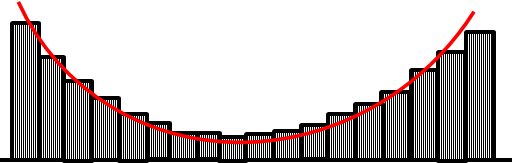
\includegraphics[width=3cm]{images/quadratic_estimation_simulation_histogram.jpg}
            \caption{二分类估计模拟直方图}
            \label{fig:二分类估计模拟直方图}
            \end{figure}
            % \textcolor[rgb]{1 0 0}{todo:图片:二分类估计模拟直方图}\\
            也就是说,更多的$\hat{y}$分散在两端,这样有利于我们分类,$\hat{y}$越大,样本越可能取值为1,$\hat{y}$越小,样本越可能取值为0。\\
            \ding{173}我们自然有当$\hat{y}$值越大时,$y$取值为1的可能越大的规律,而恰好有这样一个sigmoid函数$f_2$,如图(\ref{fig:sigmoid函数图像})所示
           \begin{figure}[H]
           \centering
           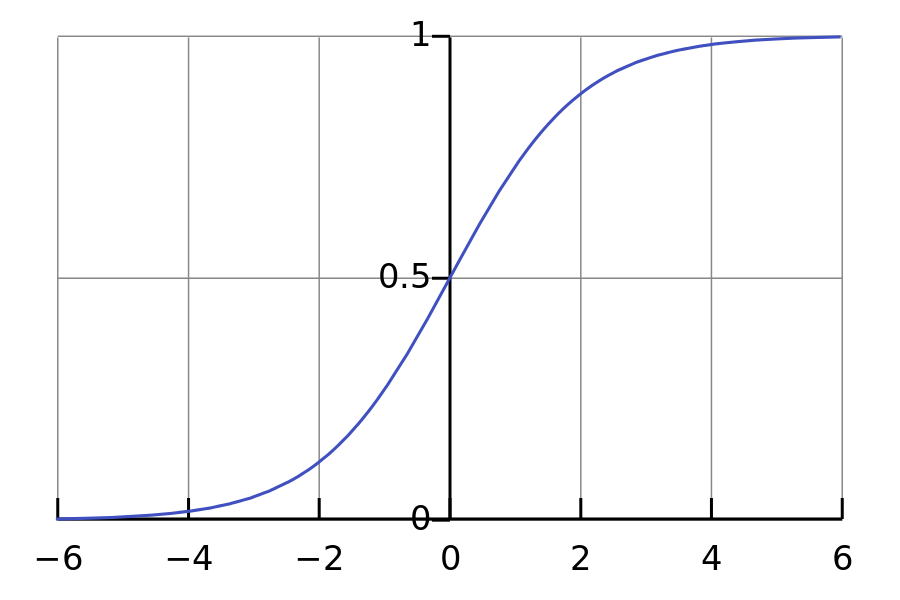
\includegraphics[width=6cm]{images/sigmoid_func.png}
           \caption{sigmoid函数图像}
           \label{fig:sigmoid函数图像}
           \end{figure}
            % \textcolor[rgb]{1 0 0}{todo:图片:sigmoid函数图像}\\
            当$\hat{y}$越小时,函数值$z$越接近0;当$\hat{y}$越大时,函数值$z$越接近1。所以,我们不能仅局限于$\hat{y} = f_1(x) = w^\mathrm{T}\phi(x)$,还应该再进行一次函数变换$f_2 = sigmoid$,于是,整个回归变为
            \begin{align*}
            \hat{y} &= f_2(f_1(x))\\
            &= f_2(w^\mathrm{T}\phi(x))\\
            &= \frac{1}{1+e^{-w^\mathrm{T}\phi(x)}}
            \end{align*}
            如果我们把上面的$\hat{y}$视为样本$y=1$的条件概率,于是有
            \begin{align*}
            P(y=1|x) = \frac{1}{1+e^{-w^\mathrm{T}\phi(x)}}\\
            =\frac{1}{1+\frac{1}{e^{w^\mathrm{T}\phi(x)}}}\\
            =\frac{e^{w^\mathrm{T}\phi(x)}}{e^{w^\mathrm{T}\phi(x)}+1}
            \end{align*}
            推得
            \begin{align*}
            & \frac{1}{P(y=1)} = \frac{1}{e^{w^\mathrm{T}\phi(x)}}+1 \\
            \Rightarrow {}&\frac{1}{P}-1 = \frac{1}{e^{w^\mathrm{T}\phi(x)}} \\
            \Rightarrow {}&\frac{1}{\frac{1}{P}-1} = e^{w^\mathrm{T}\phi(x)}\\
            \Rightarrow {}&\frac{P}{1-P} = e^{w^\mathrm{T}\phi(x)}
            \end{align*}
            于是有了我们常见的Logistic回归模型
            \begin{align*}
            \ln \frac{P}{1-P} = w^\mathrm{T}\phi(x)
            \end{align*}
            \par
            从另一个角度来看,$w^\mathrm{T}\phi(x)$的取值范围为$R$,而$y\in \{0,1\}$。我们要把二者对应起来,$P(y=1)$的取值范围为$[0,1]$,那么
            \begin{align*}
            \frac{P(y=1)}{1-P(y=1)} \in (0,\infty)
            \end{align*}
            再对上式取$\log$,其值的范围就变为$R \equiv (-\infty,\infty)$,即
            \begin{align*}
            \log \frac{P}{1-P}  \in R
            \end{align*}
            \par
            接下来的工作是:目标函数(损失函数)的确定以及优化算法的设计。
        \subsubsection{模型参数估计}
            \par
            上面建立的logistic回归方程为
            \begin{align*}
            P(y=1|x) &= f_2(w^\mathrm{T}\phi(x))\\
            &= \frac{1}{1+e^{-w^\mathrm{T}\phi(x)}}
            \end{align*}
            将其写为概率形式
            \begin{align*}
            P(y_i=1|x_i) = p_i
            = \frac{1}{1+e^{-w^\mathrm{T}\phi(x_i)}}
            \end{align*}
            看到这个单样本的条件概率分布,我们就会想到极大似然估计,我们求使样本的联合概率密度最大的$w$。由于$y_i\in \{0,1\}$,所以上式也可以写出$y_i$的条件密度
            \begin{align*}
            P(y_i|x_i) = p_1^{y_i}(1-p_i)^{1-y_i}
            \end{align*}
            \par
            为了处理方便,仍然假设样本独立同分布,于是它们的联合概率密度(似然函数)为
            \begin{align*}
            L(w|x) = \prod_{i=1}^mP(y_i|x_i) = \prod_{i=1}^mp_i^{y_i}(1-p_i)^{1-y_i}
            \end{align*}
            对上式取对数,有
            \begin{align*}
            \log L(w|x) &= \sum_{i=1}^m[y_i\ln p_i + (1-y_i)\ln (1-p_i)]\\
            &=\sum_{i=1}^m\left[ y_i\ln \frac{p_i}{1-p_i} + \ln(1-p_i) \right]
            \end{align*}
            \par
            我们的目标是求上面的对数似然函数的极大值点,即
            \begin{align*}
            \max_w\ \log L(w|x)
            \end{align*}
            将
            \begin{align*}
            p_i = \frac{e^{w^\mathrm{T}\phi(x_i)}}{1+e^{w^\mathrm{T}\phi(x_i)}}
            \end{align*}
            带入目标$\log L(w|x)$,有
            \begin{align*}
            \log L(w|x) = \sum_{i=1}^m\left[ y_iw^\mathrm{T}\phi(x_i) - \ln \left( 1+e^{w^\mathrm{T}\phi(x_i)} \right)   \right]
            \end{align*}
            对上式$w$求导,有
            \begin{align*}
            \nabla \log L(w) = \sum_{i=1}^m (y_i-p_i)\phi(x_i)
            \end{align*}
            \par
            在前面的线性回归当中,最大似然模型的极大点是解析形式的,即我们可以给出$w$的显式计算公式,这是因为对数似然函数是$w$的一个二次函数。但是对logistic回归而言,不再有解析解了,因为sigmoid($f_2$)函数是一个非线性函数。目标函数$-\log L(w)$是一个凸函数,因此优化模型存在唯一解。此外,对于$w$还有一种高效的迭代算法,这种算法是基于Newton-Raphson迭代最优框架的。为最小化$-\ln L(w) \equiv E(w)$,一般的Netwon - Raphson的权重$w$更新公式为
            \begin{align*}
            w:= w-H^{-1}\nabla E(w)
            \end{align*}
            由于
            \begin{align*}
            & \nabla E(w) = \sum_{i=1}^m(y_i-p_i)\phi(x_2)\\
            & H = \nabla\nabla E(w) = \sum_{i=1}^m y_i(1-y_i)\phi(x_i)\phi^\mathrm{T}(x_i) = \phi^\mathrm{T}R\phi
            \end{align*}
            其中:$R$是一个$m\times m$的对角矩阵,$R_{ii} = y_i(1-y_i)$,经过最优化的洗礼,$H$是什么应该是清楚的。我们看到,Hesse矩阵不再是常量,而是通过权重$R$依赖于$w$,这也解释了为什么$w$不存在解析解。使用$0 \leqslant y_i < 1$,我们看到对任意向量$u$,都有$u^\mathrm{T}u>0$(因为$H$是正定的,所以进行了Cholesby分解),因此,$E(w)$是$w$的一个凸函数。这样,logistic回归的Newton - Raphson更新公式变为
            \begin{align*}
            w:&=w-(\phi^\mathrm{T}R\phi)^{-1}\phi^{\mathrm{T}}(p-y)\\
            &= (\phi^\mathrm{T}R \phi)^{-1}(\phi^\mathrm{T}R\phi w - \phi^\mathrm{T}(p-y))\\
            &=(\phi^\mathrm{T}R\phi)^{-1}\phi^\mathrm{T}RZ
            \end{align*}
            其中:$Z$是一个$m$维向量,$Z = \phi w - R^{-1}(p-y)$。上述$w$迭代公式的形式是一组加权最小二乘问题的规范方程。由于权矩阵$R$不是常量,而是依赖于$w$。我们必须迭代地应用规范方程,每次使用新的$w$来计算$R$,然后再来求解$w$,因此,该算法被称为迭代加权最小平方算法(IRLS),是Rubin于1983年开发的。
            \par
            下面给出$E$的一个近似。和加权最小二乘问题一样,对角矩阵$R$可以看成偏差,因为logistic回归的$y$的均值和方差为
            \begin{align*}
            &E(y) = p\\
            &Var(y) =p(1-p)
            \end{align*}
            \par
            事实上,我们可以把IRLS看成变量空间$a \triangleq w^\mathrm{T}\phi(x)$的线性问题的解。这样,$Z$的第$i$个元素$Z_i$就可以简单的看成这个空间中的有效目标值。$Z_i$可以通过对当前操作点$w$附近的logistic(sigmoid)函数的局部线性近似的方法得到
            \begin{align*}
            a_i(w) :&\approx a_i(w) + \frac{\mathrm{d}a_i}{\mathrm{d}p_i} \biggl|_w(y_i-p_i) \\
            &= \phi_i^\mathrm{T}w - \frac{p_i-y_i}{p_i(1-p_i)} = Z_i
            \end{align*}
            \par
            IRLS算法步骤如下:\\
            \textbf{Step1}.初始化$w_0$,容错误差$\varepsilon$。\\
            \textbf{Step2}.计算$p_i$。对$i = 1,\dots,m$
            \begin{align*}
            p_i = p_i(w) = \frac{e^{w^\mathrm{T}\phi(x_i)}}{1+e^{w^\mathrm{T}\phi(x_i)}}
            \end{align*}
            \textbf{Step3}.计算$Z_i$。
            \begin{align*}
            E_i = \phi_i^\mathrm{T}(x_i)w - \frac{p_i-y_i}{p_i(1-p_i)}
            \end{align*}
            \textbf{Step4}.更新$w$。
            \begin{align*}
            w:=(\phi^\mathrm{T}w\phi)^{-1}\phi^\mathrm{T}RZ
            \end{align*}
            其中:$R$为对角矩阵,$R_{ii} = p_i(1-p_i)$。\\
            \textbf{Step5}.终止条件。不终止则返回Step2。
        \subsubsection{参数显著性检验}
            \par
            在前面的参数回归中,我们没有给出线性模型的系数显著性检验和拟合优度检验,而在一般的计量经济学或者统计学书籍中都会有模型参数的显著性检验以及模型检验,并且在模型估计结束后,各种统计软件(R,SPSS等)都会给出相应的检验结果。下面,我们来简单的看一下logistics回归模型的系数显著性检验和模型拟合优度检验,很明显,这里用到的是统计基础中假设检验的知识。
            \par
            上面建立的logistic回归模型为
            \begin{align*}
            P(y=1|x) = \frac{1}{1+e^{-w^\mathrm{T}\phi(x)}}
            \end{align*}
            其中:$w = (w_1,w_2,\dots,w_n)$。前面我们曾提到过,如果实际中,某一系数$w_i$不应该存在,而我们在建立模型时硬是将其设计在模型中,最后仍然会给出$w_i$的一个估计,虽然$w_i$可能不是很合理。那么,我们如何检验模型中的参数是否应该存在呢?或者说如何检验模型的合理性。我们知道,如果$w_i$不应该存在,我们就假设$w_i=0$,然后用样本数据对其进行检验。
            \par
            (1)原假设$H0:w_i = 0(i = 1,2,\dots,n)$。对于此假设,常用的检验统计量有Wald检验统计量和似然比检验统计量。Wald检验统计量为
            \begin{align*}
            T = \left[\frac{\hat{w}_i - 0}{se(\hat{w}_i)}\right]^2 \sim \chi^2(1)
            \end{align*}
            对Wald检验,当$w$的绝对值很大时,$se(w)$会膨胀,导致Wald统计量的值很小,第二类错误概率增加,应拒绝$H0$却未拒绝。为此,可以使用如下的似然比统计量
            \begin{align*}
            G = -2\ln \left( \frac{\text{不含}x_i\text{似然值}}{\text{含}x_i\text{似然值}} \right) \sim \chi^2(1)
            \end{align*}
            \par
            (2)原假设$H0:w_1 = w_2=\dots=w_n=0$。对于此假设,Wald检验统计量为
            \begin{align*}
            T = \left[\frac{\hat{w}'}{se(\hat{w}')}  \right]^2 \sim \chi^2(n)
            \end{align*}
            似然比统计量为
            \begin{align*}
            G = 2\left[ \sum_{i=1}^m y_i\ln p_i + (1-y_i)\ln (1-p_i)  \right] - [n_1\ln (n_1)+n_0\ln(n_0)-n\ln n] \sim \chi^2(n)
            \end{align*}
            其中:$n_0$表示样本中$y_i=0$的样本数。
        \subsubsection{拟合优度检验}
            \par
            我们常用模型的离差平方和来衡量估计值与真实值之间的接近程度,下面,给出3个用于评价模型好坏的度量\\
            (1)对数似然函数值
            \begin{align*}
            -2\log L = -2 \sum_{i=1}^m y_i\ln \frac{p_i}{y_i}+ (1-y_i)\ln \left( \frac{1-p_i}{1-y_i} \right)
            \end{align*}
            $-2\log L $越大,似然函数值越小,拟合效果越差。\\
            (2)AIC。AIC(1973)是Akaike's Information Criterion的缩写,计算形式为
            \begin{align*}
            AIC = -2\log l + 2(k+s)
            \end{align*}
            其中:$k$为自变量个数,$s$为反应变量类别总数减1。多模型比较时,值越小,说明模型越好。\\
            (3)SC。SC是Schnarts Criterion的缩写,是AIC的改进,其计算形式为
            \begin{align*}
            SC = -2\log L + 2(k+s)-\ln (n)
            \end{align*}
            \par
            此外,对于分类模型,我们还有混淆矩阵(错分矩阵)和ROC曲线等评价准则,我们会在决策树章节进行介绍。\\
            注:估计量$w$的渐进方差和协方差可以有信息矩阵的逆估计出来,设信息矩阵为
            \begin{align*}
            I = \frac{\partial^2L(w)}{\partial w_j\partial w_l}
            \end{align*}
            则方差为
            \begin{align*}
            & Var(\hat{w}) = I^{-1} \\
            & SE(\hat{w}_j) = (Var(w_j))^{\frac{1}{2}} \quad j = 1,2,\dots,n
            \end{align*}

    \subsection{偏最小二乘logistic回归}
        \par
        无论是多元线性回归还是上面介绍的logistic回归,都可能存在共线性问题。关于共线性问题,我们建立的线性回归模型为
        \begin{align*}
        y = w_0 +w_1x_1+w_2x_2+\dots+w_nx_n+\varepsilon
        \end{align*}
        如果上面的自变量$x_1,x_2,\dots,x_n$之间互相相关,那模型就不好用了,比如$x_2 = 2x_1$,那么我们就不需要$x_2$变量了,$x_2$可以完全由$x_1$来代替,而且在$w$的求解公式中,我们要求$X$是非奇异的,当$x_i,x_j$之间具有线性相关性时,$X$的行列式为0。因此,我们在建立模型之前,要假设各变量之间不相关。那么,我们如何检验各变量之间的相关性呢?对于这个问题,可以依据前面介绍的变量相关性检验方法。另一个问题是:我们如何检验模型的共线性呢?这个问题可以参考基础的计量经济学书籍。下面,我们来建立偏最小二乘logistics回归,此模型是维兹和德昂赫斯于2002年提出的。我们仍然假设有$n$个自变量$x_i$和$m$个样本,并设因变量$y$的分类数目$c$类。模型共分为两大部分:第一部分是提取偏最小二乘成分,可以视为主成分分析;第二部分即为一般的logistics回归建模。
        \subsubsection{提取偏最小二乘成分}
            (1)提取第一个偏最小二乘成分$t_1$。\\
            \textbf{Step1}.分别建立因变量$y$对自变量$x_j,j =1,\dots,n$的普通(无常数项)logistics回归。在模型中,记$x_j$的回归系数为$w_{1j}^*$。\\
            \textbf{Step2}.$w_1^* = (w_{11}^*,w_{12}^*,\dots,w_{1n}^*)^T$。将$w_1^*$标准化,得$w_1$
            \begin{align*}
            w_{1j} = \frac{w_{1j}^*}{\sqrt{\sum\limits_{j=1}^n (w_{1j}^*)^2}}
            \end{align*}
            \textbf{Step3}.
            \begin{align*}
            t_1 = \frac{Xw_1}{||w_1||} = \frac{Xw_1}{w_1^\mathrm{T}w_1}
            \end{align*}
            其中:$X$为样本矩阵,$w$为向量。\\
            (2)提取第二个偏最小二乘成分$t_2$。\\
            \textbf{Step1}.
            \begin{align*}
            X = t_1p_1^\mathrm{T}+X_1
            \end{align*}
            其中:$p_1$为回归系数
            \begin{align*}
            p_1 = \frac{X^\mathrm{T}t_1}{||t_1||^2}
            \end{align*}
            $x_1$为残差矩阵。记$X_{1j}$为$X_1$的第$j$列。\\
            \textbf{Step2}.对每个$x_j$,建立$y$对$t_1,X_{1j}$的logistics回归,并记系数为$w_{2j}^*$。\\
            \textbf{Step3}.$w_2^*$标准化后得到$w_2$。\\
            \textbf{Step4}.
            \begin{align*}
            t_2 = \frac{X_1w_2}{w_2^\mathrm{T}w_2}
            \end{align*}
            (3)提取第$h$个最小二乘成分$t_h$。\\
            \textbf{Step1}.
            \begin{align*}
            X= t_1p_1^\mathrm{T}+t_2p_2^\mathrm{T}+\dots+t_{h-1}p_{h-1}^\mathrm{T}+X_{h-1}
            \end{align*}
            其中:$X_{h-1}$为残差矩阵,$X_{h-1,j}$为$X_{h_1}$的第$j$列向量,
            \begin{align*}
            p_k = \frac{X_{k-1}^\mathrm{T}t_k}{||t_k||^2}
            \end{align*}
            \textbf{Step2}.对每个$x_j$,建立$y$对$t_1,t_2,\dots,t_{h-1},X_{h-1,j}$的logistics回归,记$w_{hj}$为$X_{h-1,j}$的回归系数。\\
            \textbf{Step3}.将$w_h^*$标准化得到$w_h$。\\
            \textbf{Step4}.
            \begin{align*}
            t_h = \frac{X_{h-1}w_h}{w_h^\mathrm{T}w_h}
            \end{align*}
            \textbf{Step5}.将$t_h$表示为原始变量的线性组合
            \begin{align*}
            t_h = X\tilde{w}_h
            \end{align*}
            其中:
            \begin{align*}
            \tilde{w}_h = \prod _{k=1}^{h-1}\left( I - w_kp_k^\mathrm{T} \right) w_h
            \end{align*}
        \subsubsection{建立logistics回归}
            \par
            建立logistics回归
            \begin{align*}
            \ln \left( \frac{P(y \leqslant c|t_1,t_2,\dots,t_h)}{1-P} \right) = \beta_{0c} + \sum_{j=1}^nb_jx_j
            \end{align*}
            其中:
            \begin{align*}
            b_j = \sum_{k=1}^h\beta_j\tilde{w}_{kj}
            \end{align*}
            $\beta$为待求参数。

    \subsection{logistic回归的另一种形式}
        \par
        在前面的logistics回归中,我们将因变量$y$的标签设置为$0$和$1$,即$y_i\in \{0,1\}$,$y\in B^m$,$x\in R^{m\times n}$,即共有$n$个变量,$m$个样本,$w\in R^n$(不含常数项),$\phi = (\phi_1,\phi_2,\dots,\phi_n)$。
        \par
        现在,我们将$y$的标签改为$\{-1,1\}$,其余不变,这种标签设置和SVM中的相同。我们仍然求$y_i = 1$的概率,$y_i$取值的概率可以用下式表示
        \begin{align*}
        P(y_i|x;w) = \frac{1}{1+e^{-y_i(w^\mathrm{T}\phi(x_i))}}
        \end{align*}
        我们对上面的概率进行简单的说明:当$w^\mathrm{T}\phi(x)$很小时,\ding{172}$y_i =1$,则其概率图像如图(\ref{fig:第二种logis回归概率示意图1})
            \begin{figure}[H]
            \centering
            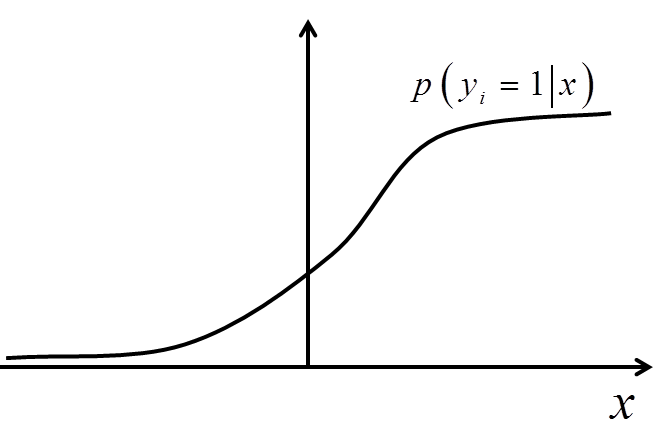
\includegraphics[height=3cm]{images/the_second_logis_regression_probability1.jpg}
            \caption{第二种logis回归概率示意图1}
            \label{fig:第二种logis回归概率示意图1}
            \end{figure}
        \ding{173}$y_i = -1$,则其概率图像如图(\ref{fig:第二种logis回归概率示意图2})
            \begin{figure}[H]
            \centering
            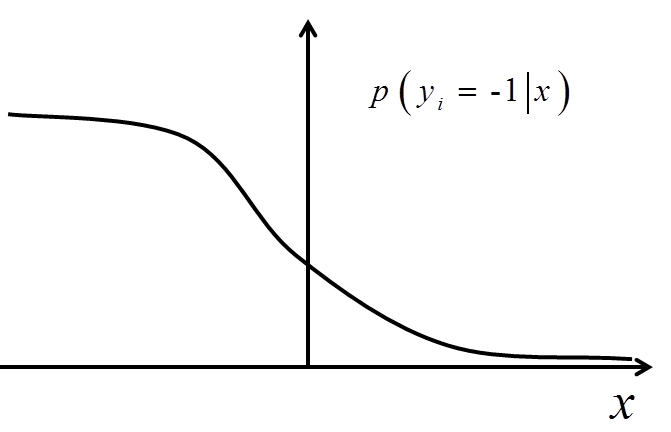
\includegraphics[height=3cm]{images/the_second_logis_regression_probability2.jpg}
            \caption{第二种logis回归概率示意图2}
            \label{fig:第二种logis回归概率示意图2}
            \end{figure}
        并且有
        \begin{align*}
        P(y_i = 1|x;w) + P(y_i = -1|x;w) = 1
        \end{align*}
        注:因为
        \begin{align*}
        &\frac{1}{1+e^{-x}}+\frac{1}{1+e^x} \\
        ={}&\frac{e^x}{1+e^x}+\frac{1}{1+e^x} \\
        ={}&1
        \end{align*}
        所以,上面的概率$P(y_i|x;w)$是合理的。写出样本的似然函数$L(w)$,有
        \begin{align*}
        L(w) = \prod_{i=1}^mP(y_i|\cdot) = \prod_{i=1}^m\frac{1}{1+e^{-y_i(w^\mathrm{T}\phi(x_i))}}
        \end{align*}
        对上式取对数,然后极大化$\log L(w)$
        \begin{align*}
        \max_w \ \log L(w) = -\sum_{i=1}^m\log\left(1+e^{-y_i(w^\mathrm{T}\phi(x_i))}\right)
        \end{align*}
        上面的问题是通常的最优化问题。我们在上面的优化目标中加入$L_2$正则化项$\frac{1}{2}||w||^2$,有
        \begin{align*}
        \min_w\ C\sum_{i=1}^m\log \left( 1+e^{-y_i(w^\mathrm{T}\phi(x_i))} \right) +\frac{1}{2}||w||^2
        \end{align*}
        其中:$\log \equiv \ln$,$C$为权重,可取$\frac{1}{m}$。上面的这个优化目标就是许多优化文章中使用的测试函数,许多SGD以及SGD改进算法都是以上面的函数作为目标。另外,scikit - learn也使用上述目标。注:关于贝叶斯logistics回归和变分logistics回归可以参考PRML相应的章节。
    \subsection{MATLAB的logistic回归示例}
        \par
        在回归模型$\hat{y} = w^\mathrm{T}x$中, At each set of values for the predictors, the response has a normal distribution with mean $\hat{y}$.
        ,在二分类logistic回归$\ln \frac{P}{1-P} = w^\mathrm{T}\phi(x)$中,$\ln \frac{P}{1-P}$是$y=1$的概率的相应的变化。更一般的,At each set of values for the predictors, the response has a distribution that can be normal, binomial, Poisson, gamma, or inverse Gaussian, with parameters including a mean $\hat{y}$,给$\hat{y}$设置一个链接函数$f$,于是得到更为一般的回归模型
        \begin{align*}
        f(\hat{y}) = w^\mathrm{T}x
        \end{align*}
        \par
        因变量$y$可能的分布有许多种,如果$y$取值为实数,可以假定其分布为正态分布,如果$y$取值为$0,1,2,...$非负整数,可以假定其分布为poisson分布,如果$y$取值为正数,可以假定其分布为逆高斯分布或者gamma分布,如果$y$取值为$0,1$,或者$0,1,2,3$(即分类型数据),则可以假定其分布为二项分布。对于不同的分布,我们可以设置不同的link(链接)函数$f$,即便对于同一种分布,也可以设置不同的链接函数。MATLAB中支持的因变量分布类型如表(\ref{tab:因变量类型及分布})所示
        \begin{table}[H]\caption{因变量类型及假设分布}
        \label{tab:因变量类型及分布}
        \centering
        \begin{tabular}{l|l}
        \toprule
        Response(y) Data Type & Suggested Model Distribution Type \\
        \midrule
        Any real number &'normal'\\
        Any positive number &'gamma' or 'inverse gaussian'\\
        Any nonnegative integer& 'poisson'\\
        Integer from 0 to n& 'binomial'\\
        \bottomrule
        \end{tabular}
        \end{table}
        \par
        对不同的假设分布类型,可选用的link函数如表(\ref{tab:假设分布及链接函数})所示
        \begin{table}[H]\caption{假设分布及链接函数}
        \label{tab:假设分布及链接函数}
        \centering
        \begin{tabularx}{\textwidth}{X|c}
        \toprule
        Value & Description\\
        \midrule
        'comploglog'                                  & $log(–log((1–\mu))) = Xb$\\
        'identity', default for the distribution 'normal'   & $\mu = Xb$\\
        'log', default for the distribution 'poisson'       & $log(\mu) = Xb$\\
        'logit', default for the distribution 'binomial'    & $log(\mu/(1 – \mu)) = Xb$\\
        'loglog'    & $log(–log(\mu)) = Xb$\\
        'probit'    & $\Phi^{–1}(\mu) = Xb$,$\Phi$ 是正态分布函数\\
        'reciprocal', default for the distribution 'gamma'  & $\mu^{–1} = Xb$\\
        p (a number), default for the distribution 'inverse gaussian' (with $p = –2$)&
        $\mu^p = Xb$\\
        \bottomrule
        \end{tabularx}
        \end{table}
        \par
        MATLAB示例如下
        \begin{lstlisting}[language = Matlab]
        x = [2100 2300 2500 2700 2900 ...
             3100 3300 3500 3700 3900 4100 4300]';
        n = [48 42 31 34 31 21 23 23 21 16 17 21]';
        y = [1 2 0 3 8 8 14 17 19 15 17 21]';
        % 构建probit回归
        g = fitglm(x,[y n],...
            'linear','distr','binomial',...
            'link','probit')
        % 自定义probit回归的链接link函数  s
        s = {@norminv,@(x)1./normpdf(norminv(x)),@normcdf};
        g = fitglm(x,[y n],...
            'linear','distr','binomial','link',s)
        \end{lstlisting}

    \subsection{多分类softmax回归}
        \subsubsection{softmax模型建立}
            \par
            前面,我们讨论了二分类问题$\{0,1\}$或者$\{-1,1\}$的logistics回归,下面,来看一下多分类问题。假设因变量$y$共$k$类,标签值为$\{1,2,\dots,k\}$,并且仍然设有$n$个自变量$x_i$,$m$个样本。如果我们对此多分类问题采用logistics回归,则可以有如下两种做法:\\
            (1)对$y$中的每个类做二分类logistics回归,例如:对于第$c$类而言,把$y = c$设置为一类,$y \neq c$设置为另一类。
            \begin{align*}
            & \ln \frac{P(y_i=1)}{1-P(y_i = 1)} = w_1^\mathrm{T}\phi(x)\\
            & \qquad \dots\\
            & \ln \frac{P(y_i=k)}{1-P(y_i = k)} = w_k^\mathrm{T}\phi(x)
            \end{align*}
            (2)我们以第$c$类为例,把$y \leqslant c$设置为一类,$y>c$设置为另一类,然后建立二分类logistics回归
            \begin{align*}
            \ln \frac{P(y_i \leqslant c)}{1-P(y_i \leqslant c)} = w_c^\mathrm{T}\phi(x)
            \end{align*}
            \par
            上面两种方法都要建立$k$个二分类logistics回归。下面,我们来介绍另一种基于logistics的多分类回归 - softmax回归。我们要求$y_i = j$的概率$P(y_i = j|x_i)$。由于$\sum\limits_{j=1}^k P(y_i = j) = 1$,那么$P(y_i = j)$等价于
            \begin{align}
            \label{softmax的y的概率分布1}
            P(y_i|x_i,w) = P_1^{I(y_i=1)}P_2^{I(y_i=2)}\cdots P_k^{I(y_i=k)}
            \end{align}
            其中:$I(y_i=j)$为特征函数,当$y_i=j$时,$I(y_i=j)=1$,否则为0;$P_k$为$P(y_i=k|x_i,w)$,且注意$a^0=1$,$0^0=1$。
            \par
            由于
            \begin{align*}
            I(y_i=k) = 1-\sum_{j=1}^{k-1}I(y_i=j)
            \end{align*}
            所以$y_i$的概率分布(\ref{softmax的y的概率分布1})可以写为
            \begin{align}
            \label{softmax的y的概率分布2}
            P(y_i|x_i,w) & = P_1^{I(y_i=1)}P_2^{I(y_i=2)}\cdots P_k^{I(y_i=k)} \\
            & = P_1^{I(y_i=1)}P_2^{I(y_i=2)}\cdots P_k^{1-\sum\limits_{j=1}^{k-1}I(y_i=j)}\notag \\
            & \xlongequal{a = e^{\log_e a}} \exp{\left(\log_e P_1^{I(y_i=1)} + \log_e P_2^{I(y_i=2)} + \cdots+\log_e P_k^{1-\sum\limits_{j=1}^{k-1}I(y_i=j)} \right)} \notag \\
            & = e^{I(y_i=1) \log P_1 + I(y_i=2) \log P_2 + \cdots + \left(1-\sum\limits_{j=1}^{k-1}I(y_i=j)\right) \log P_k}\notag \\
            & \xlongequal{\text{最后一项分散}} e^{I(y_i=1) \log (P_1/P_k) + I(y_i=2) \log (P_2/P_k) + \cdots + I(y_i=k-1) \log (P_{k-1}/P_k) + \log P_k  }\notag \\
            & = e^{\sum\limits_{j=1}^kI(y_i=j)\log P(P_j/P_k)+\log P_k}\notag \\
            & = e^{\eta^\mathrm{T}T(y_i) - a(\eta)}\notag
            \end{align}
            其中:$\eta_j = \log P_j/P_k$,$\eta = (\eta_1,\cdots,\eta_k)^\mathrm{T}$,$T(y_i) = [I(y_i=1),\cdots,I(y_i = k)]^\mathrm{T}$,$a(\eta) = \log P_k$。
            \par
            由于
            \begin{align*}
            \eta_j = \log P_j/P_k \Rightarrow P_j = P_ke^{\eta_j}
            \end{align*}
            且$\sum\limits_j P_j = 1$,可以得到
            \begin{align*}
            &\sum_j P_ke^{\eta_j} = 1\\
            \Rightarrow {}&P_k\sum_j e^{\eta_j} = 1\\
            \Rightarrow {}&P_k = \frac{1}{\sum_j e^{\eta_j}}
            \end{align*}
            于是,得到
            \begin{align*}
            P_j = P_ke^{\eta_j} = \frac{1}{\sum_je^{\eta_j}}e^{\eta_j} = \frac{e^{\eta_j}}{\sum_j e^{\eta_j}}
            \end{align*}
            \par
            现在,我们可以假设我们的模型是
            \begin{align*}
            P_j = \frac{e^{w_j^\mathrm{T}\phi}}{\sum_j e^{w_j^\mathrm{T}\phi}}
            \end{align*}
            即样本$y_i$分为$j$类的概率
            \begin{align*}
            P_j = P(y_i=j|x_i,w) = \frac{e^{w_j^\mathrm{T}\phi}}{\sum_j e^{w_j^\mathrm{T}\phi}}
            \end{align*}
            也就是说,我们在判断每一类$j$时,都有一个权重$w_j$与之对应,所以对某个样本$x_i,y_i$而言,其为$k$中各类的概率如表(\ref{tab:样本i的类别概率})所示
            \begin{table}[H]
              \caption{样本i的类别概率}
              \label{tab:样本i的类别概率}
              \centering
              \begin{tabular}{l|llll}
              \toprule
              类别             & 1       & 2      & $\dots$ & $k$\\
              \midrule
              $P_j(x_i,y_i)$   & $\cdot$ & $\cdot$&  $\frac{e^{w_j^\mathrm{T}\phi}}{\sum_j e^{w_j^\mathrm{T}\phi}}$   & $\cdot$ \\
              \bottomrule
              \end{tabular}
            \end{table}
            \par
            将softmax模型写为矢量形式(无常数项),有
            \begin{align*}
            P = f \left( \phi(x)w \right)
            \end{align*}
            矢量形式对二分类而言,$\phi(x)\in R^{m\times n}$,$w\in R^{n\times 1}$,$y\in R^{m\times 1}$,$P\in R^{m\times 1}$。对多分类而言,$\phi(x)\in R^{m\times n}$,$w\in R^{n\times k}$,$P\in R^{m\times k}$。
            \par
            至此,softmax多分类模型已经建立好了,下面的工作就是求样本的似然函数以及对数似然函数,然后求$w\in R^{n\times k}$使其似然函数最大。
        \subsubsection{softmax模型的求解}
            \par
            根据上面$y_i$的概率分布(\ref{softmax的y的概率分布1})和(\ref{softmax的y的概率分布2})我们可以写出样本$y_i(i=1,2,\dots,m)$的联合概率分布(似然函数)
            \begin{align*}
            L(w) & = \prod _{i=1}^m P(y_i)\\
            & =\prod_{i=1}^m P_1^{I(y_i=1)}P_2^{I(y_i=2)}\cdots P_k^{I(y_i=k)}\\
            & = \prod_{i=1}^m\prod_{j=1}^k \left( \frac{e^{w_j^\mathrm{T}x_i}}{\sum_je^{w_j^\mathrm{T}x_i}} \right) ^{I(y_i=j)}
            \end{align*}
            对上式取对数,有
            \begin{align}
            \label{softmax对数似然函数}
            \ln L(w) &= \sum_{i=1}^m\ln \prod_{j=1}^k \left( \frac{e^{w_j^\mathrm{T}x_i}}{\sum_je^{w_j^\mathrm{T}x_i}} \right) ^{I(y_i=j)} \notag \\
            &=\sum_{i=1}^m\sum_{j=1}^k \left( I(y_i=j) \log \frac{e^{w_j^\mathrm{T}x_i}}{\sum_je^{w_j^\mathrm{T}x_i}} \right) \notag \\
            &=\sum_{i=1}^m\sum_{j=1}^k \Bigl(I(y_i=j) \log P(y_i = j|x_i,w_j) \Bigr)
            \end{align}
            上式(\ref{softmax对数似然函数})可以看成是logistics回归的扩展,因为logistics回归的目标函数可以写为
            \begin{align*}
            \ln L(w) = \sum_{i=1}^m\sum_{j=0}^1 \Bigl(I(y_i=j) \log P(y_i = j|x_i,w) \Bigr)
            \end{align*}
            将对数似然函数(\ref{softmax对数似然函数})求导,有
            \begin{align*}
            \nabla_{w_j} \ln L(w) = \frac{\partial \ln L}{\partial w_j} &= \sum_{i=1}^m \left( \frac{\sum_j e^{w_j^\mathrm{T}x_i} }{e^{w_j^\mathrm{T}x_i}}  \frac{I(y_i = j) \cdot e^{w_j^\mathrm{T}x_i} \cdot x_i \cdot \sum_je^{w_j^\mathrm{T}x_i} - e^{w_j^\mathrm{T}x_i} \cdot e^{w_j^\mathrm{T} \cdot x_i} x_i}{ \left( \sum_je^{w_j^\mathrm{T}x_i} \right)^2  }\right)\\
            &= \sum_{i=1}^m\left[ \left( I(y_i=j)-\frac{e^{w_j^\mathrm{T}x_i}}{\sum_j e^{w_j^\mathrm{T}x_i}} \right) \cdot x_i    \right]\\
            &=\sum_{i=1}^m \Bigl[\Bigl(I(y_i=j) - P(y_i=j|x_i,w_j) \cdot x_i\Bigr)\Bigr]
            \end{align*}
            将极大似然函数估计的目标$\max\ln L(w)$变为极小化问题$\min J(w) = -\ln L(w)$,并用梯度下降、L-BFGS等算法进行求解。
            \begin{align*}
            w_j:=w_j - \alpha \nabla_{w_j} \ln L(w) \quad j=1,2,\dots,k
            \end{align*}
        \subsubsection{softmax回归求解的特点}
            \par
            softmax回归有一个特点:它有一个冗余的参数集,即$w\in \Theta$,$\Theta$是一个过大的参数集。我们从向量$w_j$出发,如果$w_j$减去一个$\psi$变为$w_j-\psi$,则softmax模型变为
            \begin{align*}
            P(y_i = j|x_i,w_j-\psi) &= \frac{e^{(w_j-\psi)^\mathrm{T}x_i}}{\sum_j e^{(w_j-\psi)^\mathrm{T}x_i}}\\
            &= \frac{e^{w_j^\mathrm{T}x_i}e^{-\psi^\mathrm{T}x_i}}{\sum_j e^{w_j^\mathrm{T}x_i}e^{-\psi^\mathrm{T}x_i}} \\
            &=\frac{e^{w_j^\mathrm{T}x_i}}{\sum_j e^{w_j^\mathrm{T}x_i}}\\
            &=:P(y_i = j|x_i,w_j)
            \end{align*}
            即$P(y_i = j|x_i,w_j-\psi) = P(y_i = j|x_i,w_j)$。换句话说,从$w_j$中减去$\psi$完全不影响预测结果,这表明softmax回归的参数空间$\Theta$是冗余的。进一步,如果$w^*$是目标函数$-\ln L(w)$的极小点,则$w^*-\psi$同样是目标函数的极小点,并且$\psi$是任意向量,因此,使$-\ln L(w)$极小化的解不是唯一的。幸运的是,由于$J(w) = -\ln L(w)$是一个凸函数,所以梯度下降算法仍然可用,不会遇到局部解。但是牛顿法以及基于牛顿法的算法则没那么幸运,其Hesse矩阵是奇异的,这导致牛顿法不能应用,因此需要用改进的L-BFGS等方法。
        \subsubsection{正则化softmax}
            \par
            我们在目标$J(w)$中引入正则项$\frac{1}{2}\sum\limits_{i=1}^m\sum\limits_{j=1}^k w_{ij}^2 $($w\in R^{n\times k}$无常数项),则我们的目标函数变为
            \begin{align*}
            J(w) = -C\left[ \sum_{i=1}^m\sum_{j=1}^k \left( I(y_i=j) \log \frac{e^{w_j^\mathrm{T}x_i}}{\sum_je^{w_j^\mathrm{T}x_i}} \right)  \right] + \frac{\lambda}{2}||w||^2
            \end{align*}
            其中:$||w||^2 = \sum\limits_{i=1}^m\sum\limits_{j=1}^k w_{ij}^2 $,$\lambda>0$为罚权重。有了$\lambda$项之后,$J(w)$就变为一个严格的凸函数,此时,就有一个唯一解$w^*$,并且Hesse矩阵变为可逆,梯度下降法、牛顿法以及L-BFGS等算法都可以使用了。目标函数$J(w)$的导数为
            \begin{align*}
            \nabla_{w_j} J(w) = -C\sum_{i=1}^m \Bigl[\Bigl(I(y_i=j) - P(y_i=j|x_i,w_j) \cdot x_i\Bigr)\Bigr] + \lambda w_j
            \end{align*}

    \subsection{人工神经网络ANN}
        \subsubsection{神经网络的导出}
            \par
            我们从前面的线性回归模型开始:对$y$的估计为
            \begin{align*}
            \hat{y} = w^\mathrm{T}\phi(x)
            \end{align*}
            在$w$给定之后,对每个样本$x_i,y_i$,都能给出其$y_i$的估计$\hat{y}_i$。现在,我们来把它改进,像前面的softmax那样,可以给出$l$个权重向量$w_j(j=1,2,\dots,l)$,每一个权重向量$w_j$都会有一个估计$\hat{y}_l = w_l^\mathrm{T}\phi(x)$,然后把$l$个线性模型进行组合。或者,从组合预测的思想来看,通过一个模型$\hat{y} = w^\mathrm{T}\phi(x)$可以给出$y$的一个估计,那么不妨多造几个模型来估计$y$,然后将这些估计值加权组合,例如
            \begin{align*}
            & \hat{y}_1 = w_1^\mathrm{T}\phi(x)\\
            & \hat{y}_2 = w_2^\mathrm{T}\phi(x)\\
            & \dots\\
            & \hat{y}_l = w_l^\mathrm{T}\phi(x)
            \end{align*}
            然后,做最终的估计
            \begin{align}
            \label{组合线性模型}
            \hat{y} = \sum_{j=1}^l \hat{y}_j \beta_j
            \end{align}
            其中:$\beta = (\beta_1,\beta_2,\dots,\beta_l)^\mathrm{T}$为组合权重。当然,还可以将每个样本赋予不同的组合权重,即$\beta$是矩阵的形式。将上式(\ref{组合线性模型})用图形表示,如图(\ref{fig:线性回归组合模型的网络示意图})所示
            \begin{figure}[H]
            \centering
            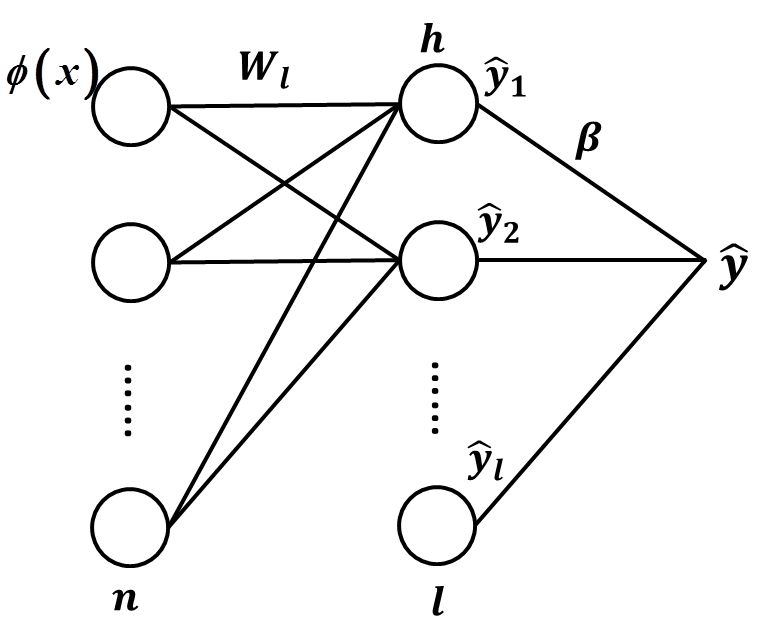
\includegraphics[height=4cm]{images/linear_regression_combination_of_network.jpg}
            \caption{线性回归组合模型的网络示意图}
            \label{fig:线性回归组合模型的网络示意图}
            \end{figure}
            \par
            对所有样本$x$而言,其模型可以写为
            \begin{align*}
            \hat{y} & = f_2f_1(x)\\
            & =f_2(w_j^\mathrm{T}\phi(x))\\
            & =\sum_{j=1}^l w_j^\mathrm{T}\phi(x)\beta_j
            \end{align*}
            上述模型即为一个简单的3层神经网络ANN。其中:$w$不再是一个单一的权重向量,而是由$l$个向量组成的矩阵,$w\in R^{n\times l}$,$w_j\in R^n$,这里共有$n$个变量,$m$个样本,$l$个线性模型,然后将它们组合。并且,由于模型结构图(\ref{fig:线性回归组合模型的网络示意图})很像人脑神经元连接形成的网络,所以这种模型被称为神经网络模型。

        \subsubsection{神经网络的讨论}
            \par
            上面,我们由线性回归组合模型引出了神经网络,下面,来研究一下神经网络ANN。\\
            (1)激活函数。在上面的网络中,我们只是确定了各个神经元的连接权重$w_{ij},\beta_j$,并没有讨论其它内容。其实,我们可以给它增加映射函数,比如我们将$x$映射为$\phi(x)$,再比如logistics回归中
            \begin{align*}
            P = f_2(f_1(x)) = f_2(w^\mathrm{T}\phi(x))
            \end{align*}
            logistics就是在$w^\mathrm{T}\phi(x)$上又增加了一个映射函数$f_2 = \frac{1}{1+e^{-x}}$。所以,我们可以在各神经元上增加映射函数,比如:$x$上增加$\phi(x)$,中间的$\hat{y}$增加$f_1$,后面的$y$再增加$f_2$,于是有
            \begin{align*}
            f_2\Bigl(\beta^\mathrm{T}f_1\big(w^\mathrm{T}\phi(x)\big)\Bigr) \rightarrow \hat{y}
            \end{align*}
            (2)阈值。其实,神经网络已经能够将$x$映射到高维,所以不妨去掉$\phi(x)$,变为$w^\mathrm{T}x$。像常见的线性回归$y=w^\mathrm{T}x + b$那样,应该有一个常数项$b \equiv w_0$。在神经网络当中,我们将$b$视为阈值$\theta$,如图(\ref{fig:神经网络阈值结构})所示的阈值结构
            \begin{figure}[H]
            \centering
            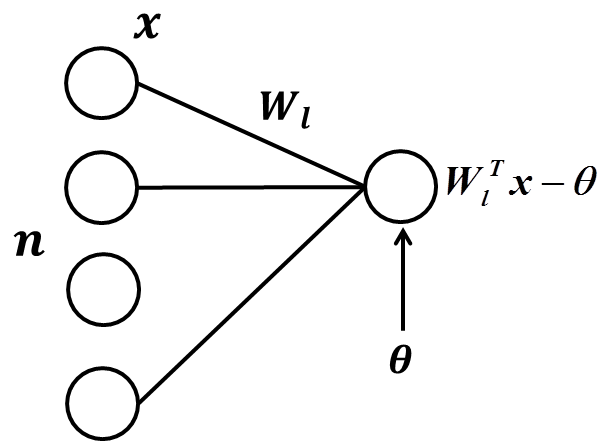
\includegraphics[height=3cm]{images/neural_network_structure.jpg}
            \caption{神经网络阈值结构}
            \label{fig:神经网络阈值结构}
            \end{figure}
            \noindent (3)多维输出问题。前面我们一直研究$y_i\in R$的问题,现在,我们来研究$x_i,y_i\in R^n\times R^p$的问题,即$n$个自变量$x$和$p$个因变量$y$之间的函数关系式。一般模型很难处理这种多维输出的问题,但对于神经网络而言,这种问题则相对简单,如图(\ref{fig:多输出问题的神经网络结构示意图})所示
            \begin{figure}[H]
            \centering
            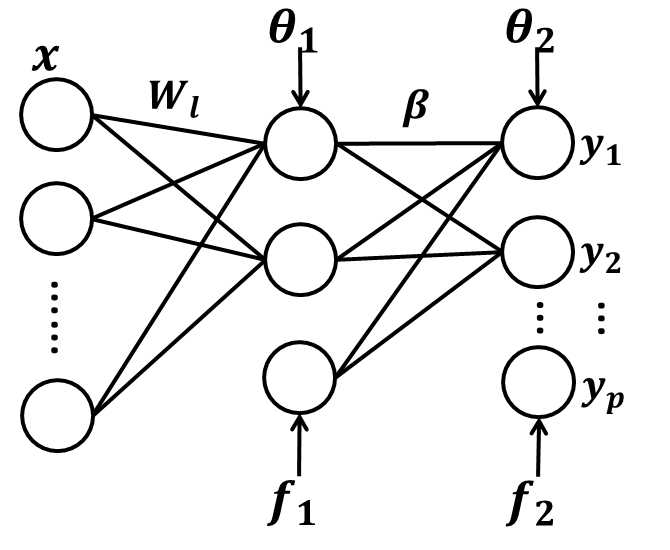
\includegraphics[height=3cm]{images/Neural_net_Structure_of_Multi_Output_Problem.jpg}
            \caption{多输出问题的神经网络结构示意图}
            \label{fig:多输出问题的神经网络结构示意图}
            \end{figure}
           像上图(\ref{fig:多输出问题的神经网络结构示意图})的网络结构,我们就处理了$f:R^n\rightarrow R^p$的多输出问题。并且,由于多分类问题是一类特别的多输出问题,因此,神经网络处理多分类问题也是容易的,我们只需要将$y^j(j=1,2,\dots,p)$设置为0和1即可,当样本为第$j$类时,$y^j = 1$,$y^i=0(i\neq j)$,这里的$p$即为多分类的种类数。\\
            (4)多层神经网络。对于前面的神经网络,它们是多个线性回归模型的组合,既然如此,我们就可以组合之后再组合。不断组合下去可以形成很深的神经网络结构,如图(\ref{fig:多层神经网络结构示意图})所示
            \begin{figure}[H]
            \centering
            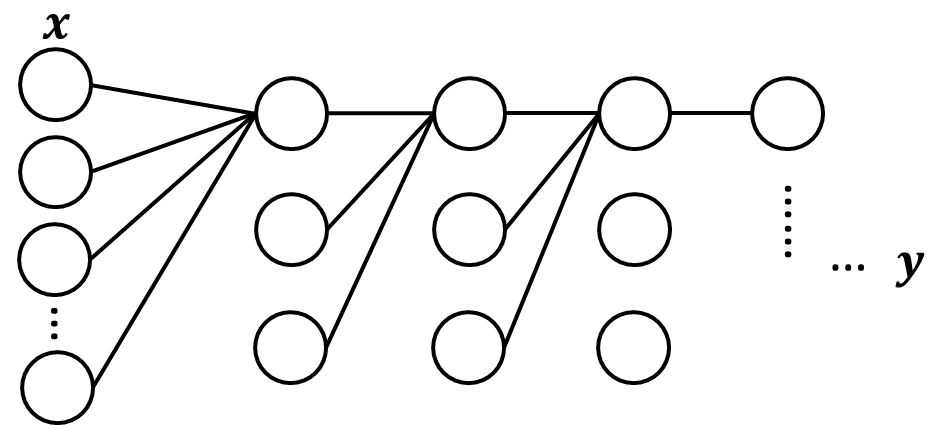
\includegraphics[height=3cm]{images/Multilayer_neural_net_structure.jpg}
            \caption{多层神经网络结构示意图}
            \label{fig:多层神经网络结构示意图}
            \end{figure}
            \par
            理论上,网络的层数可以无穷多,从而神经网络可以拟合任意任意的函数,但是,这种深层网络在实际应用时却有许多问题,比如:网络层数过多导致的过拟合现象;网络层数过多,参数$w,\theta$的求解出现问题等等。由于参数$w,\theta$的求解受限制,所以在神经网络发展初期其网络结构都非常浅(一般只有3到4层)。2006年起,由Hinton设计的DBM深层网络引发了深度网络的革命,深度学习现如今发展的如火如荼,关于深度学习问题,我们会在后面章节进行讨论。\\
            (5)网络搭建的思考。在建立一个神经网络模型时,我们应该做如下思考:\\
            \ding{172}从网络整体来看
            \begin{enumerate}
            \item 网络的输入$X$和输出$Y$是什么?
            \item 网络的层数是多少?
            \item 各层的神经元数目是多少?
            \item 映射函数/激活函数$f_1,f_2$是什么?
            \item 网络的连接形式是什么?上面给出的网络连接形式都是前一层神经元与后一层某个神经元的全链接,当然,我们可以不连接某些神经元,例如图(\ref{fig:非全连接网络结构示意图})所示
            \begin{figure}[H]
            \centering
            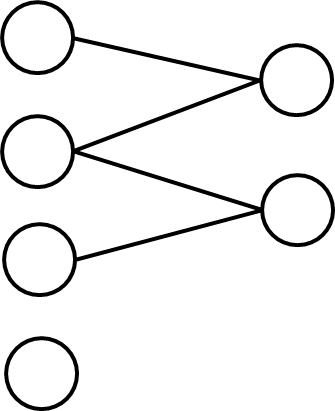
\includegraphics[height=3cm]{images/non_full_connect_net_structure.jpg}
            \caption{非全连接网络结构示意图}
            \label{fig:非全连接网络结构示意图}
            \end{figure}
            % \textcolor[rgb]{1 0 0}{todo:图片:非全连接网络结构示意图}\\
            \item 网络的训练方式,即网络参数如何求解?这个问题是重点中的重点。
            \end{enumerate}
            \ding{173}从单一神经元来看,单一神经元结构示意图(\ref{fig:单一神经元结构示意图})所示
            \begin{figure}[H]
            \centering
            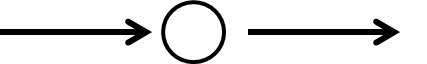
\includegraphics[width=3cm]{images/single_neuron_structure.jpg}
            \caption{单一神经元结构示意图}
            \label{fig:单一神经元结构示意图}
            \end{figure}
            \begin{enumerate}
            \item 该神经元与哪些神经元连接?
            \item 神经元的输入是什么?
            \item 神经元的输出是什么?
            \end{enumerate}
        \subsubsection{一些常用的激活函数}
            \par
            下面,我们来介绍一些常用的激活函数/传递函数$f$。像前面logistics回归中的sigmoid函数那样,我们在神经网络的各层中引入激活函数,常用的激活函数有(以$f$为函数,$x$为输入。注意这里的$x$与前面的意义不同,仅是一个符号):\\
            (1)0 - 1函数/硬阈值函数
            \begin{align*}
            f(x) =
            \left\{
            \begin{aligned}
            0 \quad x \leqslant \theta\\
            1 \quad x > \theta
            \end{aligned}
            \right.
            \end{align*}
            其中:$\theta$为阈值。MATLAB命令为hardlim。\\
            (2)线性函数
            \begin{align*}
            f(x) =ax+b
            \end{align*}
            其中:$a,b$是外来参数。MATLAB命令为purelin。\\
            (3)阈值线性函数
            \begin{align*}
            f(x) =
            \left\{
            \begin{aligned}
            & r &\quad x >\theta\\
            & ax&\quad |x|  \leqslant \theta\\
            & -r&\quad x<-\theta
            \end{aligned}
            \right.
            \end{align*}
            其中:$\theta$为阈值,$a$为外来参数。\\
            (4)sigmoid函数
            \begin{align*}
            f(x) = \frac{1}{1+e^{-x}}
            \end{align*}
            MATLAB命令为logsig。\\
            (5)tanh函数
            \begin{align*}
            f(x) = \frac{2}{1+e^{-2x}}+1 = \frac{e^{x}-e^{-x}}{e^x+e^{-x}}
            \end{align*}
            tanh函数和sigmoid很想,并且tanh的均值为0,因此,在实际应用中tanh的应用要多一些。MATLAB命令为tansig。\\
            (6)softplus
            \begin{align*}
            f(x) = \log_e(1+e^x)
            \end{align*}
            且
            \begin{align*}
            f'(x) = \frac{1}{1+e^{-x}} = sigmoid(x)
            \end{align*}
            (7)ReLu。近年来,ReLu变得越来越受欢迎,许多机器学习工具,如:Theano、TensorFlow、MXNet以及DeeplearnToolbox等几乎都使用Relu及其变形作为传递函数。Relu是线性传递函数$f=ax+b$的修正,是Rectified Linear unit的缩写,其函数形式为
            \begin{align*}
            f(x) = \max\{0,x\}
            \end{align*}
            当$x$取值比0小时,$f$的输入即为0。2005.Krizhershy等\cite{2005.Krizhershy}发现:使用Relu得到的SGD的收敛速度比sigmoid或者tanh快很多,这种现象很有可能是因为Relu是线性的。在实际的操作中,如果设置了一个很大的学习率$\eta$,那么,我们网络中的许多神经元(40$\%$)会“死亡”。下面,我们来介绍一些Relu的改进。\\
            (8)Leaky-Relu。Leaky-Relu就是用来解决Relu死机的问题,其函数形式为
            \begin{align*}
            f(x) =
            \left\{
            \begin{aligned}
            x \quad x \geqslant 0\\
            \alpha x \quad x <0
            \end{aligned}
            \right.
            \end{align*}
            其中:$\alpha$是一个很小的常数,一般取为0.001。这样即修正了数据分布,有保留了负轴上的一些值。关于Leaky-Relu的效果,有些实验证明它是成功的,当然也有一些失败了。一般的$\alpha$是人为实现赋值的,如果我们不把$\alpha$视为人为定量,而将其视为网络参数,和$w,\theta$等一起求解亦是可行的,并且Kaiming He\cite{Kaiming}指出,这种$\alpha$不仅可以训练,而且效果更好。\\
            (9)随机Relu。随机Relu是Leaky-Relu的随机版本,它将$\alpha$设置为随机变量,函数形式为
            \begin{align*}
            f(x) =
            \left\{
            \begin{aligned}
            x \quad x \geqslant 0\\
            \alpha x \quad x <0
            \end{aligned}
            \right.
            \end{align*}
            其中:$\alpha \sim U(l,\mu)$。在测试阶段,把训练过程中所有的$\alpha$求平均值,作为测试$\alpha$。\\
            (10)Max out。Goodfellow于2013年提出Max out Network。maxout的函数形式就像它的名字那样
            \begin{align*}
            f(x) = \max_i x_i
            \end{align*}
            这里顺便提一下Maxout Network,其网络的主要结构为
            \begin{align*}
            h_i(x) = \max_{j\in [1,k]} z_{ij}
            \end{align*}
            其中:$z_{ij} = x^\mathrm{T}w_{:ij}+\theta_{ij}$,$w\in R^{d\times m\times k}$。这里$w$是3维的,$d$表示输入神经元个数,$m$表示隐含层神经元个数,$k$表示每个隐含层节点对应了$k$个“隐隐含层”节点,这$k$个“隐隐含层”节点都是线性输出的,而maxout就是取这$k$个中的最大值,其结构示意图如图(\ref{fig:maxout网络结构示意图})所示
            \begin{figure}[H]
            \centering
            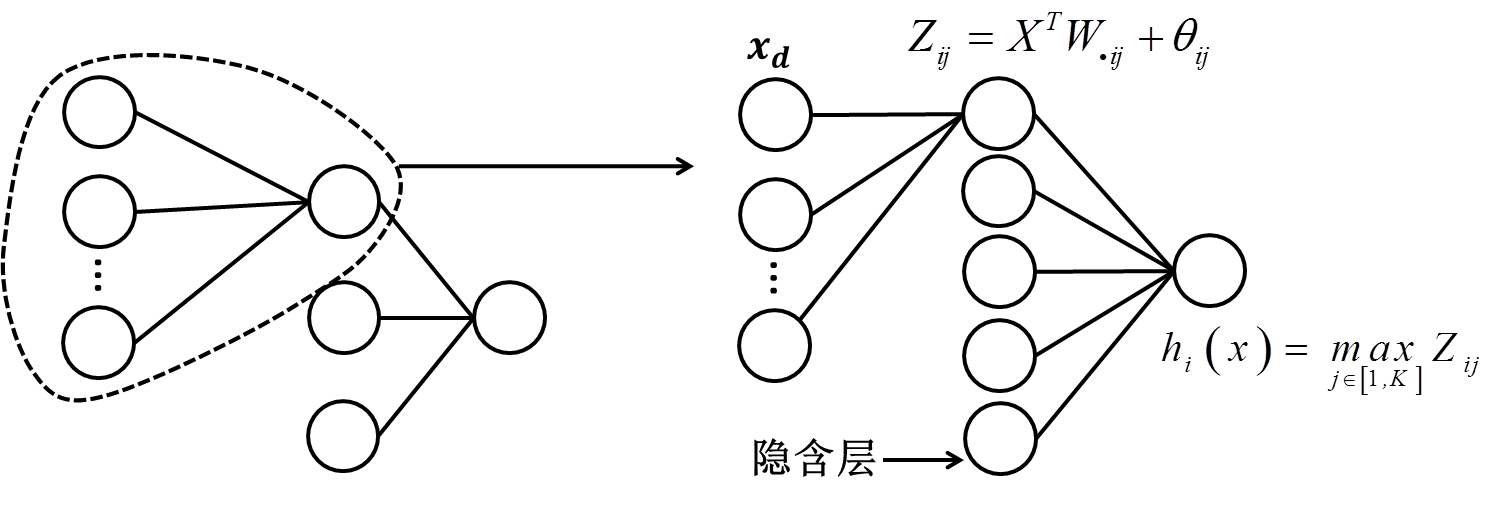
\includegraphics[height=3cm]{images/maxout_net_structure.jpg}
            \caption{maxout网络结构示意图}
            \label{fig:maxout网络结构示意图}
            \end{figure}
            \par
            常见的传递函数的图像如图(\ref{fig:传递函数图像})\footnote{此图来自维基百科}所示
            \begin{figure}[H]
            \centering
            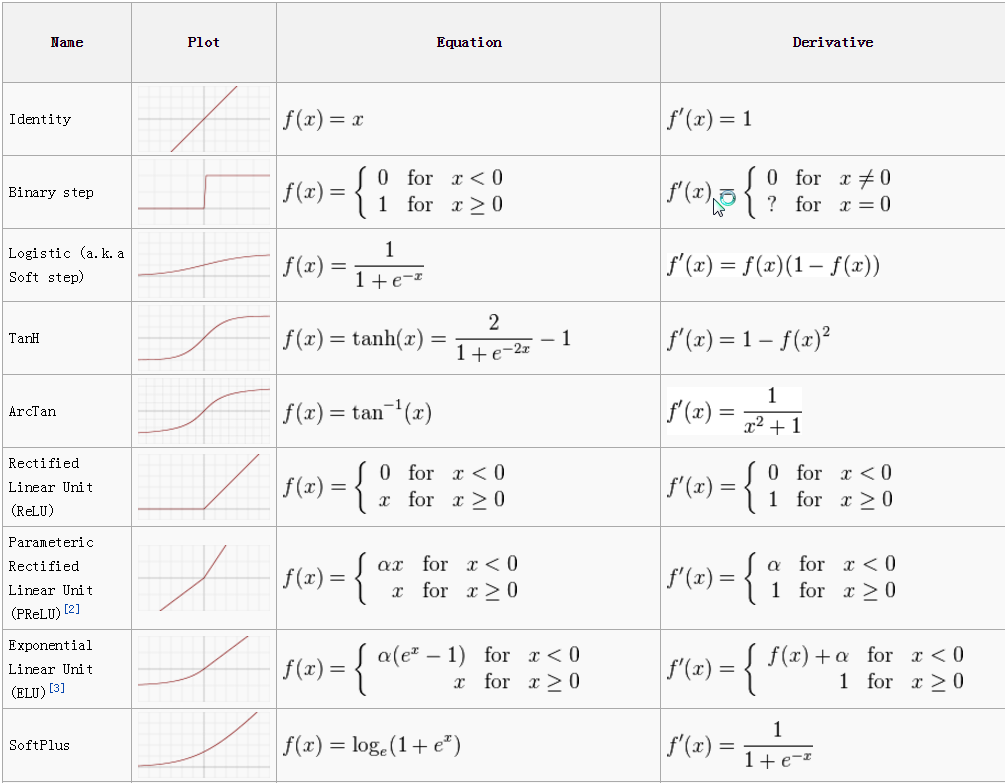
\includegraphics[width=12cm]{images/transfer_func.png}
            \caption{传递函数图像}
            \label{fig:传递函数图像}
            \end{figure}
            \par
            关于网络的学习规则,不同的网络结构有不同的学习规则,而不同的学习规则又形成了不同的网络,因此,我们将在具体的神经网络模型中讨论相应的学习规则。根据网络结构的不同,神经网络可以分为3大网络结构:前向型神经网络、竞争型神经网络和反馈型神经网络。
        % \subsubsection{神经网络前期主要研究成果}
        %     \textcolor[rgb]{1 0 0}{todo:引入--《神经网络原理》附录。}

\section{前向型神经网络}
    \subsection{感知器perception}
        \subsubsection{感知器结构}
            \par
            美国学者Frank Rosenblatt于1958年提出单层感知器,其网络结构如图(\ref{fig:单层感知器网络结构图})所示
            \begin{figure}[H]
            \centering
            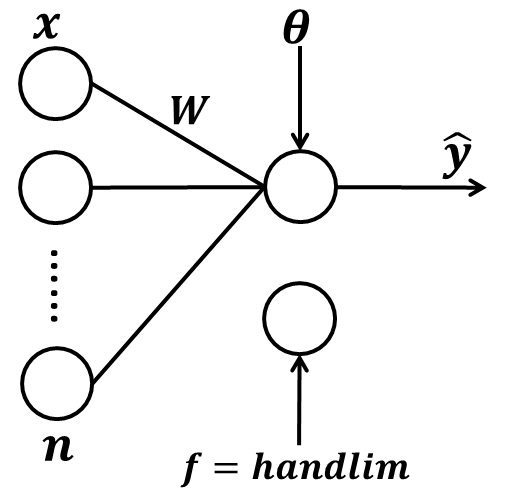
\includegraphics[height=3cm]{images/single_layer_sensor_net_structure.jpg}
            \caption{单层感知器网络结构图}
            \label{fig:单层感知器网络结构图}
            \end{figure}
                % \textcolor[rgb]{1 0 0}{todo:图片:单层感知器网络结构图}\\
                其中:$x\in R^{m\times n}$,传递函数$f = handlim$,$w\in R^n$,$y\in \{0,1\}^m$,$\theta\in R$。我们将单层感知器模型写为
                \begin{align*}
                \hat{y} = f(w^\mathrm{T}x - \theta)
                \end{align*}
                可以发现,单层感知器的功能就是对$x$进行正确的分类,且分类为$\{0,1\}$二分类,因为最终$\hat{y}$的输出值只能是0或者1。当然,我们可以用单层感知器模型来处理多分类($k$分类)问题,其结构如图(\ref{fig:单层感知器多分类网络结构图})所示
            \begin{figure}[H]
            \centering
            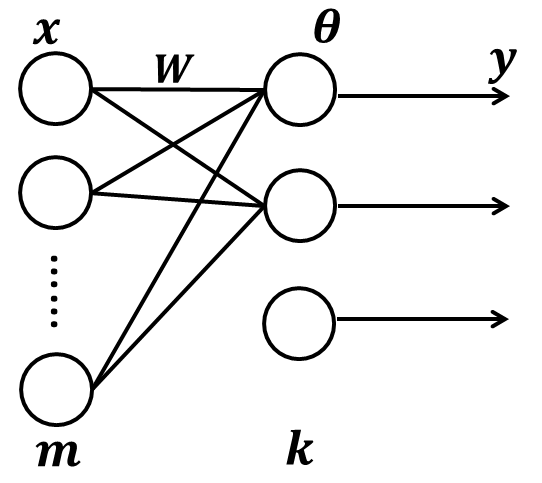
\includegraphics[height=3cm]{images/single_layer_sensor_multiple_classify_net_structure.jpg}
            \caption{单层感知器多分类网络结构图}
            \label{fig:单层感知器多分类网络结构图}
            \end{figure}
                其模型为
                \begin{align*}
                \hat{y_j} = f(s_j) &= f \left( \sum_{i=1}^n x_i w_{ij} - \theta_j \right) \\
                &=f(w_j^\mathrm{T}x-\theta_j)
                \end{align*}
            \subsubsection{感知器学习算法}
                \par
                设共有$n$个变量$x_i$和$m$个样本$(x^i,y^i)\in R^n\times R^k$,$y$为期望输出,$\hat{y}$为实际输出。\\
                \textbf{Step1}.初始化。
                输出层神经元个数$k$,初始连接权重$w(0)\in R^{n\times k}$,初始阈值$\theta$,迭代次数$t:=0$。\\
                \textbf{Step2}.对样本$x^i,y^i,i = 1,2,\dots,m$,计算该样本$x^i,y^i$的输出。
                \begin{align*}
                \hat{y}_j^i = f(w_j^\mathrm{T}x^i - \theta_j)
                \end{align*}
                \textbf{Step3}.计算实际输出$\hat{y}^i$与期望输出$y^i$的误差。
                \begin{align*}
                e^i = \hat{y}^i - y^i \in R^k
                \end{align*}
                \textbf{Step4}.调整权重及阈值。
                \begin{align*}
                & w_j:=w_j + \Delta w_j = w_j + \alpha x^i e_j \\
                & \theta:=\theta + \beta e
                \end{align*}
                其中:$\alpha,\beta$为学习率,可变化。\\
                \textbf{Step5}.所有样本完成一次更新。\\
                \textbf{Step6}.终止条件。不终止,则置$t:=t+1$,返回Step2。\\
                \textcolor[rgb]{1 0 0}{注:1.终止条件可以设置容错误差$\varepsilon$;\\
                2.
                \begin{align*}
                &x\in R^{m\times n}\times w\in R^{n\times k} - \theta\in R^{m\times 1} = \hat{y}\in \{0,1\}^{m\times k}\\
                &\hat{y}\in \{0,1\}^{m\times k} - y\in R^{m\times k} = e\in R^{m\times k}\\
                \end{align*}
                3.上述算法的目标并不是离差平方和$\sum_ie^2$最小,而仅仅是将$e$传递给$w,\theta$,后面,我们会介绍离差平方和最小方法。\\
                4.单层感知器不能解决亦或问题XOR,XOR问题的示例如图(\ref{fig:XOR问题示意图})所示
            \begin{figure}[H]
            \centering
            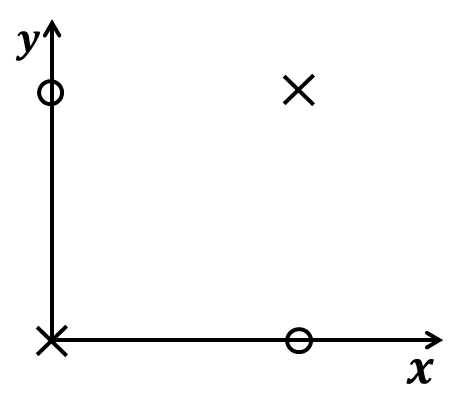
\includegraphics[height=3cm]{images/XOR_problem.jpg}
            \caption{XOR问题示意图}
            \label{fig:XOR问题示意图}
            \end{figure}
                \par
                MATLAB示例如下
                \begin{lstlisting}[language = Matlab]
                %% 单层感知器 perception
                x = [0 0 1 1;0 1 0 1];
                y = [0 1 1 1];
                net = perception;
                net = train(net,x,y);
                view(net);
                y_hat = net(x)
                \end{lstlisting}
                \par
                上面的注4中提到单层感知器不具有解决非线性分类问题XOR的能力,为此,我们可以设计多层感知器,即综合多个线性来解决非线性问题。例如:有两个单层感知器,则可以形成两条如图(\ref{fig:多层感知器解决XOR示意图})中的分割线,我们要判断各点所属的类,只要综合这两条分类线的结果即可。
            \begin{figure}[H]
            \centering
            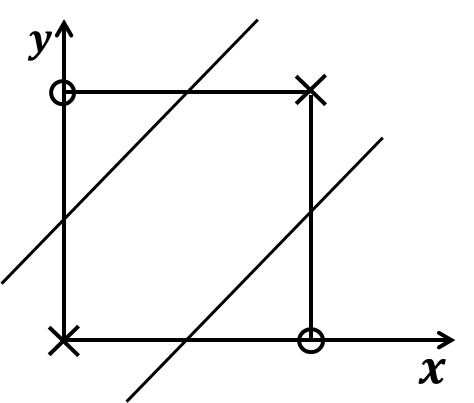
\includegraphics[height=3cm]{images/multilayer_sensor_to_solve_XOR_problem.jpg}
            \caption{多层感知器解决XOR示意图}
            \label{fig:多层感知器解决XOR示意图}
            \end{figure}
                % \textcolor[rgb]{1 0 0}{todo:图片:多层感知器解决XOR示意图}\\

                \par
                在介绍BP神经网络和反向传播算法之前,我们先来讨论一下“离差平方和最小”的目标。就像上面注2中提到的那样,对于多输出$y$,误差$e$是一个$i$行$k$列的矩阵,每个样本$i$在第$j$类处都会有个误差$e_{ij}$。如果是二分类问题和回归问题,离差平方和可以写为
                \begin{align*}
                J(w,\theta) = \sum_{i=1}^m(\hat{y}^i - y^i)^2 = ||\hat{y} - y||^2
                \end{align*}
                但是对于矩阵而言,误差$e$的离差平方和会有三种情况:\\
                (1)我们考虑将$m$个样本的离差平方和再求和,有
                \begin{align*}
                J_1(w,\theta) = \sum_{i=1}^m||\hat{y}^i - y^i||^2
                \end{align*}
                (2)考虑把$k$个输出神经元的误差求和,即先求单一的输出神经元的离差平方,然后再相加
                \begin{align*}
                J_2(w,\theta) = \sum_{j=1}^k||\hat{y}_j - y_j||^2
                \end{align*}
                (3)当然,上面两种的计算结果是一样的,为
                \begin{align*}
                J_3 (w,\theta) = \sum_{i=1}^m\sum_{j=1}^n (\hat{y}_j^i - y_j^i)^2
                \end{align*}
                \par
                很奇怪,为什么(1)(2)(3)相同还要分开写?虽然3者最终结果是一样的,但是中间步骤是不一样的,如果不看(1)(2)公式中的求和,则有$||\hat{y}^i - y^i||^2$和$||\hat{y}_j - y_j||^2$,而我们后面恰好就要着重讨论分开的形式。我们以(2)为目标,用线性神经网络来作为示例。

    \subsection{线性神经网络}
        \par
        由于感知器的输出$\hat{y}$为0和1,而$y$也为0和1,从而导致了误差$e$的元素也只有0和1。我们要想用“离差平方和最小”方法,则需要将handlim去掉,或者将其换为可导的传递函数,因为handlim对$w$求导为0。如果我们不考虑handlim函数$f$,直接将$w^\mathrm{T}x$视为$\hat{y}$,则$e = \hat{y} - y$的元素为实数。
        \par
        记第$j$个输出神经元的误差为
        \begin{align}
        \label{第j个神经元误差}
        e_j = y_j - \hat{y}_j = y_j - \left( w_j^\mathrm{T}x - \theta \right)
        \end{align}
        则第$t$次运行的均方误差为
        \begin{align}
        \label{第j个神经元的均方误差}
        E_j(w) = \frac{1}{2} ||e_j||^2 = \frac{1}{2}e_j^\mathrm{T}e_j
        \end{align}
        式(\ref{第j个神经元误差})和式(\ref{第j个神经元的均方误差})对$w$和$\theta$求导,有
        \begin{align*}
        & \frac{\partial E_j(w)}{\partial w_j} = w_j\frac{\partial e_j}{\partial w_j}= -x e_j\\
        & \frac{E_j(w)}{\partial \theta} = e_j
        \end{align*}
        其中:$x$为整个样本数据集,这一点一定要注意。由于
        \begin{align*}
        E(w) = \sum_{j=1}^k E_j(w)
        \end{align*}
        所以
        \begin{align*}
        \frac{\partial E}{\partial w_j} & = \sum_{j=1}^k \frac{\partial E_j(w)}{\partial w_j} \\
        & = -x e_j
        \end{align*}
        由此,得到权重$w$的更新公式
        \begin{align*}
        w_j:=w_j -\alpha \frac{\partial E}{\partial w_j} = w_j + \alpha x e_j
        \end{align*}

    \subsection{BP神经网络}
        \subsubsection{全BP和BP算法}
            \par
            考虑如下多层前向神经网络
            \begin{figure}[H]
            \centering
            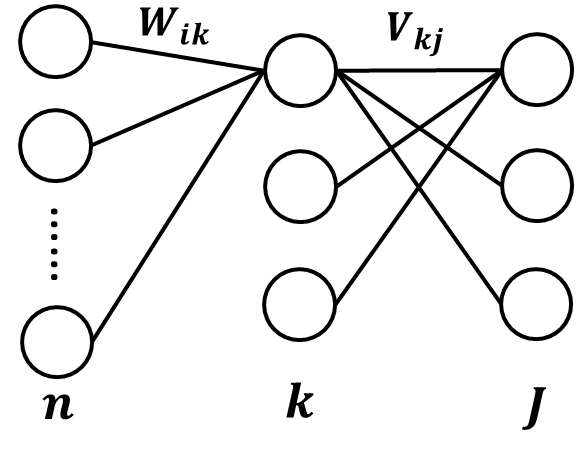
\includegraphics[height=3cm]{images/multilayer_forward_neural_network.jpg}
            \caption{多层前向神经网络}
            \end{figure}
            上面这个多层神经网络就是我们常见的神经网络。我们设定共有$n$个输入变量$x_i(i=1,2,\dots,n)$,所以输入层(第一层)共有$n$个神经元,设置隐含层(第二层)有$K$个神经元,则第一层和第二层的连接权重为$W = (w_{ik})_{n\times K}$,设置输出层(第三层)有$J$个神经元,则第二层与第三层的连接权重$V = (v_{kj})_{K\times J}$,设置隐含层的阈值为$b_1$,传递函数为$f_1(\cdot)$,输出层的阈值为$b_2$,传递函数为$f_2$。现在共有$m$个样本$(x_i,y_i)_{i=1}^m$,我们要求$W,V,b_1,b_2$。一个可行的目标是:像线性神经网络那样,使用$J$个输出神经元总误差平方和最小。设第$j$个输出神经元的误差为
            \begin{align*}
            e_j = y_j - \hat{y}_j = y_j - f_2 \left[ f_1(W^\mathrm{T}x+b_1)\cdot V_{:j} + b_2  \right]
            \end{align*}
            其中:$V_{:,j}$表示矩阵$V$的第$j$列,下面简写为$v_j$。
            则第$j$个神经元的误差平方为$E_j = \frac{1}{2}e_j^\mathrm{T}e_j$。由此,$J$个输出神经元的总误差平方为
            \begin{align*}
            E= \sum_{j=1}^J E_j = \sum_j \frac{1}{2}e_j^\mathrm{T}e_j
            \end{align*}
            我们要求$W,V,b_1,b_2$使$E$最小,则$E$对$W,V,b_1,b_2$求导,并令导数为0即可。令$\theta = \{W,V,b_1,b_2\}$,有
            \begin{align*}
            \frac{\partial E}{\partial \theta} = \sum_j \frac{\partial E_j}{\partial \theta}
            \end{align*}
            由此,我们只要求出第$j$个神经元的$E_j$关于$\theta$的导数即可。一定要注意的是,第$j$个神经元的输出为$\hat{y}_j =f_2 \left[ f_1(W^\mathrm{T}x+b_1)\cdot V_{:j} + b_2  \right]$,于是有
            \begin{align}
            \label{全BP导数计算公式1}
            \frac{\partial E_j}{\partial v_j} &= e_j\frac{\partial e_j}{\partial v_j} \notag \\
            &= e_j f_2'f_1(W^\mathrm{T}x+b_1)
            \end{align}
            也就是说,第$j$个输出神经元的误差$e_j$传递给了权重矩阵$V$的第$j$列。并且值得一提的是,求导过程要求$f_2$可导。上式的$x$是所有样本,当然,我们还可以详细的写出关于$v_{kj}$的导数,亦可以粗略写出关于矩阵$V$的导数。
            \begin{align}
            \label{全BP导数计算公式2}
            \begin{aligned}
            & \frac{\partial E_j}{b_2} = e_j f_2'\\
            & \frac{\partial E_j}{\partial W} = \frac{\partial E_j}{\partial e_j}\frac{\partial e_j}{\partial W}=e_j f_2'f_1'x\\
            & \frac{\partial E_j}{\partial b_1} = e_jf_2'f_1'
            \end{aligned}
            \end{align}
            \par
            上面给出的是参数的部分梯度(所有样本$x$的第$j$个输出神经元误差的导数方向),即$\nabla E$的一部分$\nabla E_j$。下面,我们给出总离差平方$E$下的导数,有
            \begin{align*}
            & \frac{\partial E}{\partial v_j} = \sum_j\frac{\partial E_j}{\partial v_j} = e_j f_2'f_1(W^\mathrm{T}x+b_1)\\
            & \frac{\partial E}{\partial b_2} = \sum_j\frac{\partial E_j}{\partial b_2} =\sum_j e_j f_2'\\
            & \frac{\partial E}{\partial W} = \sum_j\frac{\partial E_j}{\partial W} = \sum_j\frac{\partial E_j}{\partial e_j}\frac{\partial e_j}{\partial W} = \sum_j e_j f_2'f_1'x\\
            & \frac{\partial E}{\partial b_1} = \sum_j\frac{\partial E_j}{\partial b_1} = \sum_j e_jf_2'f_1'
            \end{align*}
            \par
            这样,我们就得到了所有样本$x$的所有输出神经元误差的导数方向,我们用梯度下降来更新参数$W,V,b_1,b_2$,使总离差平方和最小,有更新公式
            \begin{align*}
            & v_j :=v_j+\Delta v_j = v_j-\alpha \frac{\partial E}{\partial v_j}\\
            & W:=W + \Delta W = W - \alpha \frac{\partial E}{\partial W}\\
            & b_1:=b_1 -\beta \frac{\partial E}{\partial b_1}\\
            & b_2:=b_2 - \beta \frac{\partial E}{\partial b_2}
            \end{align*}
            其中:$\alpha,\beta$为学习率,可以自适应。总的来说,我们要更新某个参数$\theta$,除了要用到所有样本$x$之外,还要把所有输出神经元的梯度累加才可以。
            \par
            上面的这种做法是:$E = \sum_j E_j(j = 1,2,\dots,J)$,这里的$E_j$是第$j$个输出神经元的离差平方和。我们还可以用$E = \sum E_i(i = 1,2,\dots,m)$,这里的$E_i$是第$i$个样本的离差平方和。一个是纵向一个是横向,不过,总的来说,二者都要求在总离差梯度$\nabla_\theta E$下更新参数$\theta$,我们称这种方法为全导向传播算法(全BP)。后面介绍的BP算法是在$\nabla_\theta E_j$或者$\nabla_\theta E_i$下更新参数的。
            \par
            此外,还应该注意的是,上面的全BP(或者BP)算法是使用所有样本$x$来计算梯度的,其梯度方向是全局梯度方向,但是就像我们在回归模型中介绍SGD(以及SGD改进等)算法时所说的那样,不仅可以用全部样本$x$来计算梯度方向,还可以用部分样本(批量梯度MBGD)以及单一样本的随机梯度SGD来计算梯度方向。下面,给出一次一个样本的随机梯度SGD的BP算法的步骤:\\
            \textbf{Step1}.初始化。\\
            网路结构以及网络参数设置$W,V,b_1,b_2,f_1,f_2$,学习率$\alpha,\beta$,容许误差$\varepsilon$,迭代设置:$t:=0,T_{max}$。\\
            \textbf{Step2}.在$t$时刻,遍历所有样本$x^i,i=1,2,\dots,m$,执行Step3 - Step6。\\
            \textbf{Step3}.对样本$x^i$,按网络结构进行前向传播
            \begin{align*}
            & W^\mathrm{T}x^i\\
            & W^\mathrm{T}x^i+b_1\\
            & f_1(W^\mathrm{T}x^i+b_1)\\
            & V^\mathrm{T}f_1(W^\mathrm{T}x^i+b_1)\\
            & V^\mathrm{T}f_1(W^\mathrm{T}x^i+b_1)+b_2\\
            & f_2(V^\mathrm{T}f_1(W^\mathrm{T}x^i+b_1)+b_2) = \hat{y}^i
            \end{align*}
            \textbf{Step4}.计算样本$x^i,y^i$的误差$e^i$
            \begin{align*}
            &e^i = \hat{y}^i - y^i \in R^J\\
            &E_i = \frac{1}{2} ||e^i||^2
            \end{align*}
            $e^i$是一个向量,和$y^i$同维度,$e_j^i\in R$是第$j$个输出神经元的误差。如果是批量样本,$e_j$是一个向量。\\
            \textbf{Step5}.误差反向传播。(关于导数的计算,仿照前面全BP的计算方法(\ref{全BP导数计算公式1})和(\ref{全BP导数计算公式2}),本质是复合函数的链式求导法则)
            \begin{align*}
            & \frac{\partial E_i}{\partial V} = \frac{\partial E_i}{\partial e^i}\frac{\partial e^i}{\partial V} = e^i f_2' f_1 (W^\mathrm{T}x^i+b_1) \\
            & \frac{\partial E_i}{\partial W }= \frac{\partial E_i}{\partial e^i}\frac{\partial e^i}{\partial W} = e^i f_2'f_1'x^i    \\
            & \frac{\partial E_i}{\partial b_2} = \frac{\partial E_i}{\partial e^i}\frac{\partial e^i}{\partial b_2} = e^i f_2' \\
            & \frac{\partial E_i}{\partial b_1} = \frac{\partial E_i}{\partial e^i}\frac{\partial e^i}{\partial b_1} = e^if_2'f_1'
            \end{align*}
            \textbf{Step6}.按梯度方向更新$W,V,b_1,b_2$,使$E_i$最小
            \begin{align*}
            & V :=V+\Delta V = V -\alpha \frac{\partial E_i}{\partial V}\\
            & W:=W + \Delta W = W - \alpha \frac{\partial E_i}{\partial W}\\
            & b_1:=b_1 -\beta \frac{\partial E_i}{\partial b_1}\\
            & b_2:=b_2 - \beta \frac{\partial E_i}{\partial b_2}
            \end{align*}
            \textbf{Step7}.终止条件:$T_{max}$或者$\varepsilon$。达到最大迭代次数或者误差$e<\varepsilon$则终止;否则,置$t:=t+1$,返回Step2。
            \par
            上述BP算法是一般形式的BP算法,每次输入一个样本$x^i,y^i$,然后根据非全局误差$e^i$即$E_i$来计算梯度,更新权重等参数。由于每次使用一个样本来计算梯度,这样的梯度方向并不是全局下降方向,也就是说,此次的权重更新只能使样本$x^i,y^i$的误差$e^i$减小,而其它样本则未可知。当然我们可以选择一次输入一个样本(SGD),一次输入部分样本(MBGD)以及一次输入整个样本(GD),并且样本可以按照顺序输入,也可以随机抽取输入。一般而言,我们经常使用批量梯度下降算法,其梯度方向是使该批样本的误差下降的方向,更新后的参数并不一定能使所有样本的误差下降。
        \subsubsection{BP算法的问题及改进措施}
            \par
            BP算法存在以下几个主要的问题:
            \begin{enumerate}
            \item 收敛速度慢。由于有两层for循环,所以其迭代速度是可想而知的,并且,它对于一个简单的问题,收敛速度仍然很慢。
            \item 非全局极小点。由于不是全BP算法,并且每次使用一个样本来计算梯度,而每个样本的梯度方向不一样,会导致该样本的梯度与上一个样本梯度发生冲突,甚至梯度下降方向完全相反,从而遗忘(抵消)上一个样本的梯度方向(特征)。例如可能出现如图(\ref{fig:BP算法的锯齿梯度下降示意图})的情况
            \begin{figure}[H]
            \centering
            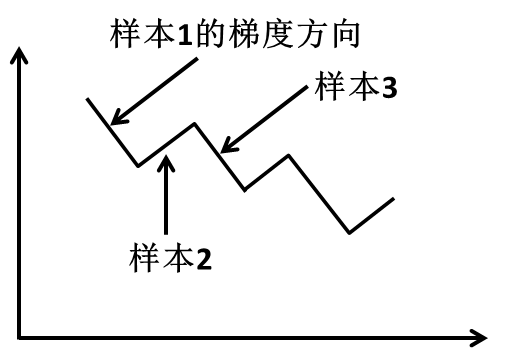
\includegraphics[height=3cm]{images/BP_algorithm_to_reduce_sawtooth_gradient.jpg}
            \caption{BP算法的锯齿梯度下降示意图}
            \label{fig:BP算法的锯齿梯度下降示意图}
            \end{figure}
            % \textcolor[rgb]{1 0 0}{todo:图片:BP算法的锯齿梯度下降示意图}
            \item 每个样本带来的梯度大小不等。先来看单一样本$x^i,y^i$的梯度
            \begin{align*}
            \frac{\partial E_i}{\partial W }= \frac{\partial E_i}{\partial e^i}\frac{\partial e^i}{\partial W} = e^i f_2'f_1'x^i
            \end{align*}
            从上面的梯度计算公式中可以看出:$W$的梯度大小和样本$x^i$的大小有关,如果$x^i$很大,则会导致其梯度方向很大。这是非常不好的,如果一个极端的(坏的)样本$x^i$带来了很大的梯度,那么,其余的样本基本上上就不起作用了,这样收敛的极小点是没有意义的。
            \end{enumerate}
            为了克服BP算法的缺点,我们介绍BP算法的一些改进措施:
            \begin{enumerate}
            \item 问题1中说BP算法的收敛速度慢,我们并不太可能改进BP的框架,那么我们就去改进它的学习率$\alpha,\beta$,给出以下3种可行的方案:
            \ding{172}让$\alpha,\beta$在$\Delta W$前后相差不大(即前后梯度方向相似的)时较大;\ding{173}让$\alpha,\beta$在平均梯度方向上较大;\ding{174}当前后两次的梯度方向符号一致时,增大$\alpha,\beta$。
            \item 问题2中说BP算法会遗忘上一个样本的梯度,那我们此次的梯度方向就不仅用此次样本的误差下降方向,再加上上一次的量,有
            \begin{align*}
            \Delta W := -\alpha\frac{\partial E}{\partial W} + \eta \Delta W
            \end{align*}
            也就是说权重更新量$\Delta W$不仅与梯度$\frac{\partial E}{\partial w}$有关,而且还与其上一个样本的梯度方向有关,这种方法被称为动量梯度下降方法。
            \item 问题3中说BP算法的梯度大小受样本大小的影响,为此,我们在将样本输入到网络之前,先对其进行\textbf{归一化处理}。归一化处理的本质工作是将样本值压缩,避免样本有太大的差异。归一化有许多方法,这里我们不详细介绍。MATLAB中使用mapminmax来实现如下归一化
            \begin{align*}
            x = \frac{x-x_{min}}{x_{max} - x_{min}}
            \end{align*}
            \par
            并通过参数'apply'和'reverse'来分别指定归一化和反归一化操作,例如:x=mapminmax('apply',x),就是对x进行归一化操作。
            \end{enumerate}
            \par
            上面,我们用SGD等随机优化算法来求解了BP神经网络。可以看出,BP神经网络最终仍然是一个最优化问题,并且是一个最小二乘优化问题,我们仍然可以用一些一般性的算法,比如牛顿法、F-BFGS算法以及L-M算法等。下面,我们简单的介绍一些参数更新方案:\\
            (1) GD
            \begin{align*}
            W(t+1)= W(t)-\alpha \frac{\partial E(t)}{\partial W(t)}
            \end{align*}
            (2)动量因子momentum
            \begin{align*}
            & \Delta W(t+1)= \alpha(1-\eta)\frac{\partial E(t)}{\partial W(t)} + \eta \Delta W(t)\\
            & W(t+1)=W(t)+\Delta W(t+1)
            \end{align*}
            (3)变学习率算法
            \begin{align*}
            &\alpha(t+1)=
            \left\{
            \begin{aligned}
            k_{inc}\alpha(t) \quad E(t+1)<E(t)\\
            k_{doc}\alpha(t) \quad E(t+1)>E(t)
            \end{aligned}
            \right.
            \\
            &\eta(t+1)=
            \left\{
            \begin{aligned}
            &1.05\eta(t) \quad E(t+1)<E(t)\\
            &0.7\eta(t)\quad E(t+1)>1.04E(t)\\
            &\eta(t)
            \end{aligned}
            \right.
            \end{align*}
            (4) RPROP
            \begin{align*}
            \Delta W(t+1) = \Delta W(t+1) \cdot \mathrm{sign}[g(t)] =
            \left\{
            \begin{aligned}
            & \Delta W(t)k_{inc} \cdot \mathrm{sign}[g(t)] \quad\text{连续两次梯度方向相同}\\
            & \Delta W(t)k_{doc} \cdot \mathrm{sign}[g(t)] \quad\text{连续两次梯度方向相反}\\
            & \Delta W(t)
            \end{aligned}
            \right.
            \end{align*}
            其中:$g(t) = \frac{\partial E(t)}{\partial W(t)}$。\\
            (5) CG(Conguga gradient)
            \begin{align*}
            & p(0) = -q(0)\\
            & W(t+1) = W(t) + \alpha p(t)\\
            & p(t) = -g(t) + \beta(t)p(t-1)
            \end{align*}
            对于$\beta(t)$,\ding{172}Fletcher-Reeres(CGF)的计算方法是
            \begin{align*}
            \beta(t) = \frac{g^\mathrm{T}(t)g(t)}{g^\mathrm{T}(t-1)g(t-1)}
            \end{align*}
            \ding{173}Polck - Ribiere(CGP)的计算方法是
            \begin{align*}
            \beta(t) = \frac{\Delta g^\mathrm{T}(t-1)g(t)}{g^\mathrm{T}(t-1)g(t-1)}
            \end{align*}
            (6) Newton
            \begin{align*}
            W(t+1) = W(t) - H^{-1}(t)g(t)
            \end{align*}
            其中:$H$为Hesse矩阵。海赛矩阵不易求解,转而有OSS和Quasi-Newton等算法。\\
            (7) LM(levenberg-marquardt)
            \par
            由于误差$E$具有平方和误差的形式,为最小二乘优化问题,我们有
            \begin{align*}
            & H \approx J^\mathrm{T}J\\
            & g = J^\mathrm{T}e
            \end{align*}
            其中:$J$是$E$对权重$W$一阶导数,雅可比矩阵。有权重更新公式
            \begin{align*}
            W(t+1) = W(t) - J^\mathrm{T}J +\mu JJ^{-1}J^\mathrm{T}e
            \end{align*}
            当$\mu=0$时为牛顿法。

            \begin{table}[htbp]
              \caption{MATLAB中的BP算法命令表}
              \label{tab:MATLAB中的BP算法命令表}
              \centering
              \begin{tabular}{l l l}
              \toprule
              简称     & 函数命令   & 描述                                     \\
              \midrule
              LM       & trainlm    & 基于Levenberg-Maruardt算法的BP算法       \\
              BFG      & trainbfg   & 基于BFGS Quasi-Newton算法的BP算法        \\
              GDX      & traingdx   & 自适应学习率以及动量梯度下降BP算法       \\
              GDA      & traingda   & 自适应学习率的梯度下降BP算法             \\
              GDM      & traingdm   & 自适应学习率的梯度下降BP算法             \\
              GD       & traingd    & 梯度下降BP算法                           \\
              OSS      & trainoss   & One Step Secant BP算法                   \\
              RP       & trainrp    & RPROP Resilient反向传播(反弹)          \\
              SCG      & trainscg   & 按比例缩小的共轭梯度下降BP算法           \\
              CGB      & traincgb   & Powell Beale restarts 共轭梯度下降BP算法 \\
              CGF      & traincgb   & Fletcher Reeves updates共轭梯度下降BP算法\\
              CGP      & traincgp   & Polak - Ribiere 变梯度BP算法             \\
              \bottomrule
              \end{tabular}
            \end{table}
            \par
            MATLAB中提供了许多种BP算法,如表(\ref{tab:MATLAB中的BP算法命令表})所示。表中各种算法的特点可以参见《MATLAB神经网络43个案例分析》P392或者《MATLAB神经网络应用设计》P87。上述算法的本质都在寻找梯度下降方向,并没有改变BP算法的大的算法结构,也没有改变神经网络的网络结构。对于BP神经网络框架的改进,可以尝试下面几个方向:
            \begin{enumerate}
            \item 初始网络权重的改进。在前面的BP算法中,网络参数$W,V,b_1,b_2$的初始值是随机设置的,这种做法会导致网络收敛速度较慢,可以使用GA等优化算法挑选一些合适的初始值,然后再运行BP网络。
            \item 网络节点的改进。一般的BP网络中,各层神经元个数是事前确定的。这里,我们可以将网络中神经元的个数也归入到网络优化当中,使用GA等算法进行预先求解。
            \item 神经元连接方式的改进。一般的BP神经网络各层神经元之间采用全连接的形式,我们可以采用部分连接的形式,也可以尝试随机连接的形式。
            \item 传递函数$f_1,f_2$的改进。下面,我们将介绍一种小波神经网络,这种网络就是将传递函数$f_1,f_2$设置为小波函数$g$。一个关键的问题是小波函数$g$的求导。
            \end{enumerate}
            \par
            注:关于神经网络的逼近能力(拟合能力),Hecht-Nielsen证明了如下Kolmogorov定理:
            \begin{theorem}[Kolmogorov定理]
            $\forall f:U\to R\in C^1$,$f$可以精确的用3层前馈神经网络实现。
            \end{theorem}
        \subsubsection{MATLAB示例}
            \par
            MATLAB提供了许多神经网络函数命令,下面,我们简单的介绍一些网络。\\
            \ding{172}fitnet用于函数拟合,其调用格式为
            \par
            net = fitnet(hiddenSize,train,Fcn)
            \par
            示例:
            \begin{lstlisting}[language = Matlab]
            [x,y] = simplefit.dataset;
            net = fitnet(10);
            view(net)
            net = train(net,x,y);
            y_hat = net(x);
            perf = perform(net,y_hat,y)
            \end{lstlisting}
            \ding{173}feedforwardnet用于构建前馈神经网络,其调用格式为
            \par
            net = feedforwardnet(hiddenSize,train,Fcn)
            \par
            示例:
            \begin{lstlisting}[language = Matlab]
            net = feedforwardnet(10);
            net = train(net,x,y);
            view(net);
            y_hat = net(x);
            perf = perform(net,y_hat,y)
            \end{lstlisting}

    \subsection{小波神经网络}
        \par
        todo:待补充。。。
        % \textcolor[rgb]{1 0 0}{todo:引入:某个书上的小波神经网络}
    \subsection{RBF径向基神经网络}
        \par
        当网络的一个或多个可调参数($W,b$)对任何一个输出都有影响时,称该类网络为全局逼近网络。由于每输入一个样本,权重都要调整一次,从而导致了全局逼近网络的学习速度很慢,比如前面介绍的BP神经网络。如果对于输入空间的某一个局部区域只有少数几个链接权值影响输出,则称该网络为局部逼近网络。常见的局部逼近网络为RBF网络、小脑模型CMAC和B样条网络等,下面,我们就来介绍RBF径向基神经网络。
        \subsubsection{RBF径向基插值}
            \par
            设共有$m$个样本$x_i,y_i(i=1,2,\dots,m)$,$x_i,y_i\in R^n\times R$。多变量插值可以表述为:寻找一个函数$F:R^n\rightarrow R$,满足
            \begin{align*}
            F(x_i) = y_i \quad i= 1,2,\dots,m
            \end{align*}
            \par
            上面表述的插值问题是严格的插值问题,它要求插值函数$F$经过$n$个样本点。径向基函数插值就是构造如下形式的插值函数
            \begin{align*}
            F(x) = \sum_{i=1}^m w_i \varphi(||x-x_i||)
            \end{align*}
            其中:$\{\varphi ||x-x_i||\}_{i=1}^m$是$m$个函数的集合,称为径向基基组,$\varphi||x-x_i||$称为径向基,$||\cdot||$表示范数,$x_i$为径向基$\varphi||x-x_i||$的中心。当然,径向基$\varphi$的个数可以不是$m$。
            \par
            乍一看,径向基插值函数和支持向量机很像,一个是核函数$K(x,x_i)$,一个是径向基函数$\varphi(||x-x_i||)$。但是径向基函数是完全插值问题,要求$F(x_i) = y_i$
            \begin{align*}
            & \sum_{i=1}^mw_i\varphi(||x_1 -x_i||) = y_1\\
            & \sum_{i=1}^mw_i\varphi(||x_2 -x_i||) = y_2\\
            & \qquad \dots\\
            & \sum_{i=1}^mw_i\varphi(||x_m -x_i||) = y_m
            \end{align*}
            将上式表述为矩阵的形式,有
            \begin{align*}
            \begin{pmatrix}
            \varphi_{11} & \varphi_{12}& \dots & \varphi_{1m} \\
            \varphi_{21} & \varphi_{22}& \dots & \varphi_{2m} \\
            \vdots&\vdots&\ddots&\vdots\\
            \varphi_{m1} & \varphi_{m2}& \dots & \varphi_{mm} \\
            \end{pmatrix}
            \begin{pmatrix}
            w_1\\
            w_2\\
            \vdots\\
            w_m
            \end{pmatrix}
            =
            \begin{pmatrix}
            y_1\\
            y_2\\
            \vdots\\
            y_m
            \end{pmatrix}
            \end{align*}
            其中:$\varphi_{ij} = \varphi(||x_i-x_j||)$,$i,j=1,2,\dots,m$。即
            \begin{align*}
            \phi w = y
            \end{align*}
            其中:$\phi = \{\varphi_{ij}\}_{i,j=1}^m$。
            \par
            我们要求$w$,如果$\phi$为非奇异矩阵,则$\phi^{-1}$存在,那么$w = \phi^{-1}x$。接下来的问题是:如何保证矩阵$\phi$是非奇异的呢?
            \par
            可以证明,对大量径向基函数$\varphi$,在某些条件下,上述问题的答案为:(1986.Micchelli定理)
            如果$\{x_i\}$是$m$个互不相同的点的集合,则$m\times m$阶矩阵$\phi$是非奇异的。有大量的径向基函数满足Micchelli定理,比如:\\
            (1)多二次函数
            \begin{align*}
            \varphi(r) = (r^2+c^2)^\frac{1}{2} \quad \text{对某些}c>0,r\in R
            \end{align*}
            (2)拟多二次函数(Inverse multiquadrics)
            \begin{align*}
            \varphi(r) = \frac{1}{(r^2+c^2)^\frac{1}{2}}
            \end{align*}
            (3)高斯函数
            \begin{align*}
            \varphi(r) = e^{-\frac{r^2}{2\sigma^2}}
            \end{align*}
            (4)Reflected Sigmoid
            \begin{align*}
            \varphi(r)=\frac{1}{1+e^{\frac{r^2}{\sigma^2}}}
            \end{align*}
            \par
            上面的拟多二次函数和高斯函数都是局部函数,当$r\rightarrow \infty$时,$\varphi(r)\rightarrow 0$,并且二者的$\phi$矩阵是正定的。我们将上面的径向基函数$F(x) = \sum\limits_{i=1}^mw_i\varphi(||x-x_i||)$绘制成神经网络的形状,其网络结构图如图(\ref{fig:RBF网络结构图})所示
            \begin{figure}[H]
            \centering
            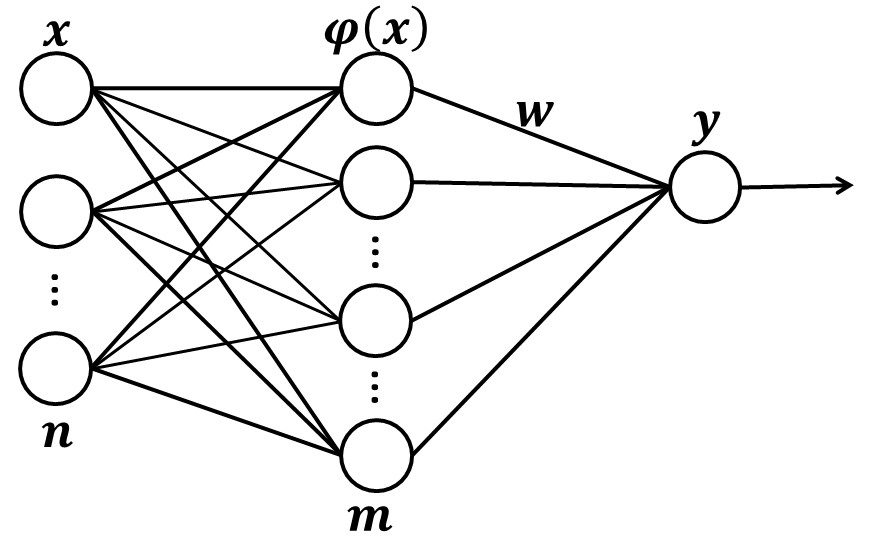
\includegraphics[height=3cm]{images/RBF_net_stucture.jpg}
            \caption{RBF网络结构图}
            \label{fig:RBF网络结构图}
            \end{figure}
            % \textcolor[rgb]{1 0 0}{todo:图片:RBF网络结构图}\\
            我们知道每个样本$x_i(i=1,2,\dots,m)$都会是一个径向基函数$\varphi$的中心,其对应于RBF网络结构图(\ref{fig:RBF网络结构图})的中间层有$m$个神经元,每一个为$\varphi(x_i)(i=1,2,\dots,m)$。
            \par
            在介绍RBF网络的训练算法之前,我们来看一下RBF网络的缺点:
            \begin{enumerate}
            \item 插值函数$F(x)$会经过所有样本点$(x_i,y_i)$,当样本中包含噪声(坏点/坏样本)时,RBF会拟合出一个坏的曲面$F$,从而使网络的泛化能力下降,由于输入样本$x_i$中含有坏样本,我们就想挑选一些样本来做基$\varphi$的中心,而那些坏样本不能做$\varphi$的中心,这样,$F$就不会经过“坏点”了。将径向基网络中间层的神经元个数设置为$k(k<m)$,即从样本集中挑选$k$个作为基中心,则RBF可以写为
            \begin{align*}
            F(x) = \sum_{i=1}^k w_i \varphi(||x-x_i||)
            \end{align*}
            至于如何从样本集中挑选$k$个样本,留在后面讨论(主要目的是去掉样本中的坏点)。
            \item 基函数个数等于训练样本数目时,当样本数目$m$很大时,远超于物理过程中有的自由度,问题就把那位超定了,$\phi$可能不稳定。我们采用正则化方法解决这个问题。
            \end{enumerate}
            \par
            上面我们建立了RBF网络,下面要讨论的问题是:1.隐含层神经元个数以及径向基中心,即如何从样本集中选取$k$个样本作为径向基中心;2.径向基函数中的参数如何确定;3.RBF网络的训练方法。
        \subsubsection{RBF的求解}
            \par
            首先,我们来解决径向基中心$x_i(i = 1,2,\dots,k)$的选取问题。我们的目标是从$m$个样本中选出$k$个,使这$k$个样本能够尽可能反应$m$个样本的特征。聪明如我,马上就能想到用K - means聚类方法来选择$k$个样本中心,如果我们能通过K均值聚类来挑选$k$个径向基中心,那么想必其它聚类算法(无监督方法)也是可行的。但是在用K均值聚类时,我们仍然要确定聚类中心数/径向基中心数$k$,至于如何确定$k$,我们不做讨论。假设我们已经得到了$k$和$k$个径向基中心$x_i$,下面我们来求解权重$w = (w_1,w_2,\dots,w_k)^\mathrm{T}$。
            \paragraph{方法1:最小二乘法}由于我们把径向基的个数从$m$调整为$k$,所以$\phi$不再是一个方阵,$w$不能像前面的$\phi^{-1}y$那样求解了。和前面参数回归部分处理的方法一样,我们将$\phi^{-1}$处理成$\phi$的广义逆(伪逆)$\phi^\dag$,于是有
            \begin{align*}
            w= \phi^\dag y
            \end{align*}
            其中:$\phi^\dag = (\phi^\mathrm{T}\phi)^{-1}\phi^\mathrm{T}$,$\phi^\mathrm{T}\phi$是一个方阵。我们令$R = \phi^\mathrm{T}\phi$ ,$r= \phi^\mathrm{T}y$。
            \paragraph{方法2:递归最小二乘方法}上述最小二乘方法使用的是非常普遍的。但是,当隐含层神经元个数$k$很大时,求$(\phi^\mathrm{T}\phi)^{-1}$会是一个非常吃力的工作,因此,我们有必要对矩阵进行改造。令$R = \phi^\mathrm{T}\phi$ ,$r= \phi^\mathrm{T}y$,则原回归问题写为
            \begin{align*}
            &\phi^\mathrm{T}\phi w = \phi^\mathrm{T}y \\
            \Rightarrow{} &Rw = r
            \end{align*}
            其中:$R$定义为$k\times k$相关函数,$r$称为互相关向量。我们将$r$重写,对$n = 1,2,\dots,m$,有
            \begin{align}
            \label{r计算公式1}
            r(n) & = \sum_{i=1}^{n-1} \phi(x_i)y_i + \phi(x_n)y_n\notag \\
            & =r(n-1)+\phi(x_n)y_n\notag\\
            & =R(n-1)w(n-1)+\phi(x_n)y_n
            \end{align}
            其中:
            \begin{math}
            \phi(x_i) =
            \left[
             \begin{smallmatrix}
            \varphi(x_i,x_1)\\
            \vdots\\
            \varphi(x_i,x_k)
            \end{smallmatrix}
             \right] \in R^k
            \end{math}
            。在上面的第一个等式中,将$i=n$单独提取处理,在最后一个等式中,用$r(n-1) = R(n-1)w(n-1)$代替$r(n-1)$。
            \par
            在式(\ref{r计算公式1})的右边加上$\phi(n)\phi^\mathrm{T}(n)w(n-1)$,然后再减去它,有
            \begin{align}
            \label{r计算公式2}
            r(n) & = R(n-1)w(n-1)+ \phi(x_n)y_n + \phi(n)\phi^\mathrm{T}(n)w(n-1) - \phi(n)\phi^\mathrm{T}(n)w(n-1)\notag\\
            & = \Bigl( R(n-1)+\phi(n)\phi^\mathrm{T}(n) \Bigr) w(n-1)+\phi(n) \Bigl( y_n-\phi^\mathrm{T}(n)w(n-1) \Bigr)
            \end{align}
            上式(\ref{r计算公式2})的$R(n-1)+\phi(n)\phi^\mathrm{T}(n) = R(n)$是相关函数,而$y_n-\phi^\mathrm{T}(n)w(n-1)$称为先验估计误差。这里使用“先验”是为了强调估计误差$\alpha(n)$是基于权重向量$w(n-1)$的老估计。回到(\ref{r计算公式2})中
            \begin{align*}
            r(n) = R(n)w(n-1) + \phi(n)\alpha(n)
            \end{align*}
            将上述方程带入$r(n) = R(n)w(n)$中,有
            \begin{align*}
            R(n)w(n) = R(n)w(n-1)+\phi(n)\alpha(n)
            \end{align*}
            于是有
            \begin{align*}
            w(n) = w(n-1) + R^{-1}(n) \phi(n)\alpha(n)
            \end{align*}
            上述问题的关键是:如何求解$R^{-1}(n)$。
            \par
            我们已经知道
            \begin{align*}
            R(n) = R(n-1)+\phi(n)\phi^\mathrm{T}(n)
            \end{align*}
            那么对于$R^{-1}(n)$,可以通过迭代算法进行求解。先引入矩阵逆的计算
            \begin{lemma}[矩阵逆的计算]
            设矩阵$A$为
            \begin{align*}
            A = B^{-1}+ CDC^{\mathrm{T}}
            \end{align*}
            其中:$B$为非奇异矩阵,$B^{-1}$存在,$A,B$有相同的维度,$D$为一非奇异矩阵。则$A^{-1}$为
            \begin{align*}
            A^{-1} = B-BC(D+C^\mathrm{T}BC)^{-1}C^\mathrm{T}B
            \end{align*}
            \end{lemma}
            \par
            根据上述矩阵逆的引理,我们有
            \begin{align*}
            R^{-1}(n) = R^{-1}(n-1) - \frac{R^{-1}(n-1)\phi(n)\phi^\mathrm{T}(n)R^{-1}(n-1)}{1+\phi(n)R^{-1}(n-1)\phi(n)}
            \end{align*}
            这里,我们在方程右端第二项利用了相关矩阵的对称性$R^\mathrm{T} = R$。
            \par
            下面,我们各处RBF的递归最小二乘算法。为了书写方便,我们引入两个新的变量
            \begin{align*}
            & R^{-1}(n) = p(n)\\
            & g(n) = R^{-1}(n)\phi(n)= p(n)\phi(n)
            \end{align*}
            称$g(n)$为增益向量,因为$w(n) = w(n-1)+g(n)\alpha(n)$。RBF递归最小二乘算法为:\\
            \textbf{Step1}.初始化。\\
            训练样本$\{\phi(i),y(i)\}$,$w(0) := 0$,$p(0) = \lambda ^{-1}I$,容错误差$\varepsilon$,径向基个数$k$。\\
            \textbf{Step2}.计算径向基中心$x_j(j = 1,2,\dots,k)$。\\
            \textbf{Step3}.确定高斯径向基$\varphi(r) = e^{-\frac{r^2}{2\sigma^2}}$的参数$\sigma$
            \begin{align*}
            \sigma_j = \frac{c_{max}}{\sqrt{2k}} \quad j= 1,2,\dots,k
            \end{align*}
            其中:$c_{max}$为选取中心$x_j$的最大距离。\\
            \textbf{Step4}.对样本$n = 1,2,\dots,m$进行如下计算
            \begin{align*}
            & p(n) = p(n-1) - \frac{p(n-1)\phi(n)\phi^\mathrm{T}(n)p(n-1)}{1+\phi^\mathrm{T}(n)p(n-1)\phi(n)}\\
            & g(n) = p(n)\phi(n)\\
            & \alpha(n) = y(n) - w^\mathrm{T}(n-1)\phi(n)\\
            & w(n) = w(n-1)+g(n)\alpha(n)
            \end{align*}
            \textbf{Step5}.终止条件。不终止则返回Step4。
            \par
            注意:初始值$p(0) = \lambda^{-1} I$,$\lambda$是小的正常数,是基于如下正则化目标
            \begin{align}
            \label{RBF正则化目标}
            J(w) = \frac{1}{2} \sum_{i=1}^m \left( y_i - w^\mathrm{T}\phi_i \right) ^2 + \frac{1}{2}\lambda ||w||^2
            \end{align}
            \paragraph{方法3:LMS算法}
            一般的,我们研究以(\ref{RBF正则化目标})为目标的LMS算法,我们将正则化项去掉,求$w$使$J(w)$最小
            \begin{align*}
            \min_w \ J(w) & = \frac{1}{2} \sum_{i=1}^m \left( y_i - w^\mathrm{T}\phi_i \right) ^2 \\
            & = \frac{1}{2}\sum_{i=1}^m e_i^2
            \end{align*}
            其中:$e_i$为样本$x_i,y_i$的误差。
            \par
            现在,我们不仅要求$w$使$J(w)$最小,还要求径向基中心$c$和高斯径向基的外来参数(“超参数”)$\sigma$使$J(w)$最小。整理一下RBF模型
            \begin{align*}
            y & = w^\mathrm{T}\varphi(||x-c||)\\
            & =\sum_{j=1}^k w_j\varphi(||x-c_j||)\\
            & =\sum_{j=1}^k w_j\exp \left( -\frac{1}{2\sigma_j^2}||x-c_j|| \right)
            \end{align*}
            其中:$k$为径向基个数,$\varphi$为径向基函数,$\varphi(x) = \exp \left( -\frac{1}{2\sigma_j^2}||x-c_j|| \right) $为高斯径向基,$\sigma_j$为径向基超参,$c_j$为径向基中心。
            \par
            所以,我们现在不仅要求$w_j$使$J(w,c,\sigma)$最小,还要求$c_j$和$\sigma_j$使$J(w,c,\sigma)$最小。将$J(w,c,\sigma)$关于参数$\theta = (w,c,\sigma)$求导,有
            \begin{align*}
            \frac{\partial J}{\partial \theta} = \frac{1}{2} \sum_{i=1}^m \frac{\partial e_i^2}{\partial \theta} = \sum_{i=1}^m e_i \frac{\partial e_i}{\partial \theta}
            \end{align*}
            所以,只需要求每个样本$x_i,y_i$的残差$e_i$关于参数$\theta$的导数即可,有
            \begin{align*}
            e_i = y_i - \sum_{j=1}^k w_j\exp \left( -\frac{1}{2\sigma_j^2}||x_i-c_j|| \right)
            \end{align*}
            \par
            为使$J(w)$最小,参数修正量$\Delta \theta$与梯度方向$\nabla_\theta$相反,于是有
            \begin{align*}
            & \Delta c_j = \eta \frac{w_j}{\sigma_j^2} \sum_{i=1}^m e_i \varphi (||x_i-c_j||)(x_i-c_j)\\
            & \Delta \sigma_j = \eta \frac{w_j}{\sigma_j^2} \sum_{i=1}^m e_i \varphi (||x_i-c_j||)||x_i-c_j||^2\\
            & \Delta w_j = \eta \sum_{i=1}^m e_i\varphi (||x_i-c_j||)
            \end{align*}
            \par
            上述梯度方向是所有样本的梯度方向,是全局梯度(即GD),在算法编程的表现是:当所有样本循环一遍之后才更新一次权重参数。当然,我们也可以使用梯度下降SGD(一次一个样本)和批量梯度下降MBGD(一次部分样本)来加快收敛速度。对于SGD的一次一个样本而言,记样本为$x_l,y_l$,则目标为
            \begin{align*}
            \min \ E(\theta)  = \frac{1}{2} e_l^2
            \end{align*}
            并且有如下参数更新公式
            \begin{align*}
            & \Delta c_j = \eta \frac{w_j}{\sigma_j^2} e_l \varphi (||x_l-c_j||)(x_l-c_j)\\
            & \Delta \sigma_j = \eta \frac{w_j}{\sigma_j^2} e_l \varphi (||x_l-c_j||)||x_i-c_j||^2\\
            & \Delta w_j = \eta  e_l\varphi (||x_l-c_j||)
            \end{align*}
            注:2002.Rifkin博士论文中细致的比较了基于RLS算法的RBF和SVM在线性可分模式下的性能,实验表明:\ding{172}RLS和SVM近乎相同;\ding{173}二者都对异常样本点敏感,在USPS数据集上,RLS和SVM在ROC曲线上一样的好甚至更好,在MIT人脸识别上,SVM比RLS要好。
        \subsubsection{MATLAB示例}
            \par
            MATLAB中提供了两个径向基网络:newrb和newrbe,并提供了径向基函数radbas。\\
            \ding{172}newrb用来设计一个approximate径向基网络,其调用格式为
            \par
            net = newrb(x,y,goal,spread,MN,DF)\\
            其中:x是一个$n\times m$输入矩阵;y是一个$p\times m$的目标矩阵;goal是MSE的容错程度,默认为0;spread是径向基函数的扩展速度;MN是神经元最大数目;DF是两次显示之间所添加的神经元数目。\\
            \ding{173}newrbe用于设计一个精确径向基网络,其调用格式为
            \par
            net = newrbe(x,y,spread)
            \par
            示例:
            \begin{lstlisting}[language = Matlab]
            x = [1,2,3];
            y = [2.0,4.1,5.9];
            net = newreb(x,y);
            %net = newrb(x,y);
            x_new = 1.5;
            y_hat = sim(net,x_new);
            \end{lstlisting}
    \subsection{广义回归网络GRNN}
        \par
        广义回归网络GRNN是美国学者Donald.F.Specht于1991年提出的网络结构,具有很强的非线性映射能力和高度的容错性和鲁棒性,适用于非线性函数拟合、逼近问题。GRNN在逼近能力和学习速度上较RBF有更强的优势,网络(函数)最终收敛于样本量积聚较多的回归面,并且在样本量较少时效果也很好。
        \par
        在前面的RBF中,我们曾经提到过径向基函数$\varphi$和核函数是相似的,下面我们来看一下非参数核回归和RBF之间的关系。在非参数回归部分,我们介绍了一些非参数回归方法,其中就有N-W常系数核权重回归,其回归式为
        \begin{align*}
        \hat{y} = \hat{f}(x) = \frac{\sum\limits_{i=1}^m y_i K \left( \frac{x-x_i}{h} \right)  }{\sum\limits_{j=1}^m  K \left( \frac{x-x_j}{h} \right) }
        \end{align*}
        其中:$h$为窗宽,$x_i\in R^n$,共有$m$个样本和$m$个核。我们令
        \begin{align*}
        W_{hi}(x) = \frac{K \left( \frac{x-x_i}{h} \right)}{\sum\limits_{j=1}^m K \left( \frac{x-x_j}{h} \right)}
        \end{align*}
        则有
        \begin{align}
        \label{NW非参数回归}
        \hat{y} = \sum_{i=1}^m y_i W_{hi}(x)
        \end{align}
        且权重和为1,即$\sum_i W_{hi} = 1$。
        \par
        下面,我们将RBF网络中的径向基函数$\varphi$也归一化
        \begin{align*}
        \varphi(x) = \frac{\varphi \left( \frac{||x-x_i||}{h} \right)   }{\sum\limits_{j=1}^m \varphi \left( \frac{||x-x_i||}{h} \right)}
        \end{align*}
        用归一化径向基$\varphi$来重新构建RBF模型,有
        \begin{align}
        \label{GRNN网络}
        F(x) = \sum_{i=1}^m w_i \varphi(x) = \frac{\sum\limits_{i=1}^m w_i \exp \left( -\frac{||x-x_i||}{2\sigma^2} \right)  }{\sum\limits_{j=1}^m \exp \left( -\frac{||x-x_j||}{2\sigma^2} \right) }
        \end{align}
        其中:$\varphi(x)$为归一化的径向基函数。上面式(\ref{GRNN网络})即为广义回归神经网络DRNN,MATLAB中是用newgrnn来实现GRNN的,其调用格式为
        \par
        net = newgrnn(x,y,spread)

\section{竞争型神经网络}
    \subsection{自组织特征映射SOM}
        \subsubsection{SOM网路结构}
            \par
            自组织特征映射网络(self-Organizing Feature Map)是一种无监督学习算法,由芬兰赫尔辛基大学教授Kohonen于1981年提出,所以也称为Kohonen网络。SOM可用于语音识别、图像处理、组合优化和数据分析等众多领域。
            \par
            前面我们讨论的神经网络都属于有监督学习模型,并且网络神经元的连接有一个特点是:只有上下层神经元的连接,某一层的各神经元之间不连接,如图(\ref{fig:层间连接示意图})所示
            \begin{figure}[H]
            \centering
            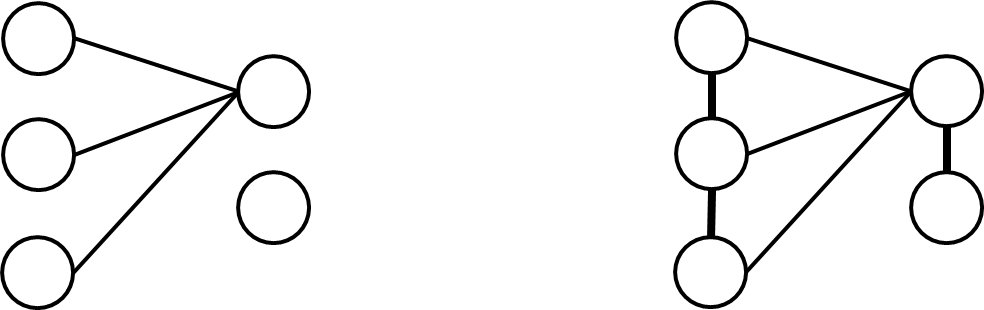
\includegraphics[height=3cm]{images/Interconnection.jpg}
            \caption{层间连接示意图}
            \label{fig:层间连接示意图}
            \end{figure}
            \par
            常用的SOM神经网络由输入层和输出层(竞争层)组成,输入层各神经元通过权重将外界信息(样本)汇集到输出层各神经元。输出层神经元与输入层神经元全连接,输入层和输出层内部神经元不连接,输出层内的每个神经元与其邻近的神经元连接,连接时互相激励的作用,训练后,输出层不同神经元节点代表不同的分类模式,所以SOM的输出层也叫做特征映射层。
            \par
            竞争层神经元的排列方式可以是一维的、二维的也可以是高维的,甚至还可以是不规则排列的。下面图(\ref{fig:输出层二维排列的SOM})给出了输出层二维排列的SOM。
            \begin{figure}[H]
            \centering
            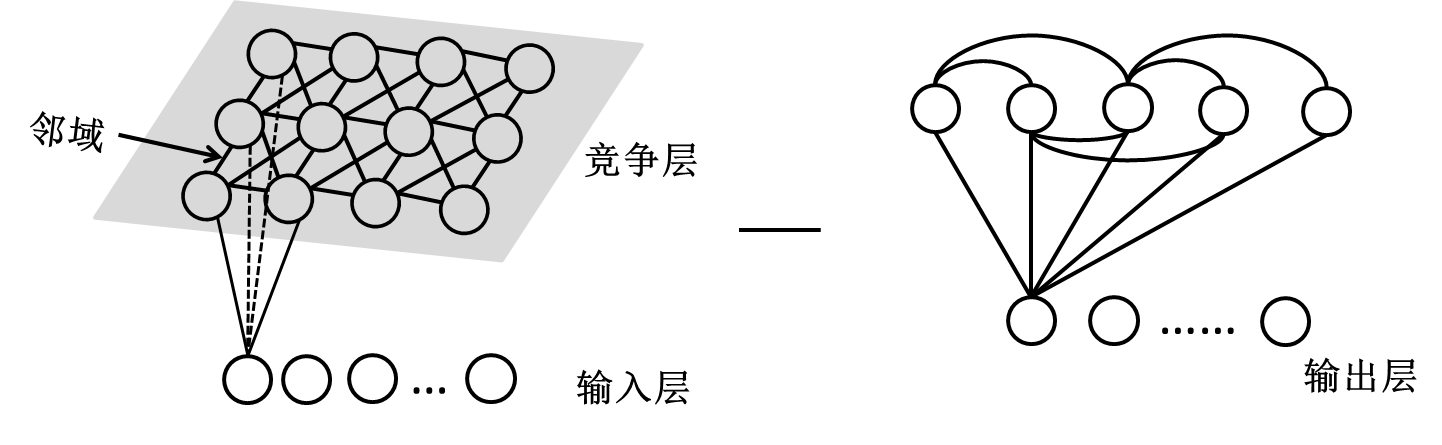
\includegraphics[height=3cm]{images/Output_layer_two_dimensional_arrangement_of_SOM.jpg}
            \caption{输出层二维排列的SOM}
            \label{fig:输出层二维排列的SOM}
            \end{figure}
            其中:输入层神经元个数为$n$,竞争层神经元个数为$k\times k = K$个,二维输出层上的各神经元之间可以是全连接,也可以是局部连接。SOM的目标是在无监督(无$y$)的情况下,从输入数据中找出规律,网络通过自身训练自动对输入模式(样本)进行分类。
        \subsubsection{SOM学习算法}
            \par
            上面介绍了SOM的网络结构,下面介绍它的学习算法。SOM学习算法包含竞争、合作和更新3个过程:\\
            (1)竞争过程:在竞争过程中,确定输出最大的神经元为获胜神经元。就单一神经元来看,由于神经元的激励函数(传递函数)是线性的,所以神经元的输出值的大小取决于神经元的输入$u_i = \sum_j w_{ij}x_j$,即输入向量$x$和权重$W$的内积(注:权重矩阵用$W,W_1,V$等表示,矩阵元素用$w_{ij}$表示,矩阵某行某列用$W_{:j} = w_j$表示)。而该内积最大在输入向量和权重均为归一化时,等价于$x,W$的欧几里得距离最小,所以,当输入向量为$x$,且第$l$个神经元获胜时,满足条件
            \begin{align*}
            ||x-w_l|| = \min_{1 \leqslant i \leqslant K} ||x-w_i||
            \end{align*}
            (2)合作过程:确定获胜神经元的加强中心。以在竞争过程中获胜的神经元为中心,设置邻域大小,在邻域范围内的神经元称为兴奋神经元,即加强中心。\\
            (3)更新过程:采用Hebb学习规则对权重进行更新。
            \par
            SOM学习算法的步骤如下:\\
            \textbf{Step1}.初始化。\par
            输入层神经元个数$n$,输出层神经元个数$K$,初始连接权重$w(0)$,竞争神经元$j$个邻接神经元集合$S_j$,$S_j(0)$是随机的,$S_j(t)$随迭代次数$t$不断减小,置$t:=0$。\\
            \textbf{Step2}.将一个样本$x=(x_1,x_2,\dots,x_n)^\mathrm{T}$输入到网络。\\
            \textbf{Step3}.计算欧几里得距离$d_j$。\par
            输入样本与每个输出神经元$j$之间的欧几里得距离
            \begin{align*}
            d_j = ||x-w_j|| = \sqrt{\sum_{i=1}^n\Big(x_i(t) - w_{ij}(t)\Big)^2}
            \end{align*}
            其中:$w_j$表示矩阵的第$j$列。计算出最小距离对的神经元$j^*$
            \begin{align*}
            j^* = \arg \min_{1 \leqslant j \leqslant K} \{d_j\}
            \end{align*}
            \textbf{Step4}.给出获胜神经元$j^*$的一个邻域$S_{j^*}(t)$。按下式修正获胜神经元$j^*$及其“邻接神经元”的权值
            \begin{align*}
            w_{ij}(t+1) =w_{ij}(t) + \eta(t)[x_i(t) - w_{ij}(t)]
            \end{align*}
            其中:$\eta$为学习率,可以是$\eta(t) = \frac{1}{t}$。\\
            \textbf{Step5}.计算输出$y_k$
            \begin{align*}
            y_k = f(\min_j ||x - w_j||)
            \end{align*}
            其中:$f$为激励函数,可以是$0,1$函数也可以是线性函数。\\
            \textbf{Step6}.终止条件。如果不终止,则返回Step2.
        \subsubsection{MATLAB应用实例}
            \par
            MATLAB提供selforgmap来实现SOM网络,其调用格式为
            \par
            selforgmap(dimensions,cowerSteos,initNeighbor,topolugyFun,distanceFcn)\\
            其中:dimensions是行向量维数,默认为$8\times 8$;coverSteps Number of training steps for initial covering of the input space, 默认为100;initNeighber为初始邻域大小;topologyFcn为层拓扑函数,默认为'hextop';distanceFcn为距离函数,默认为'linkdist'。函数示例如下
            \begin{lstlisting}[language = Matlab]
            x = simplecluster_dataset;
            net = selforgmap([8,8]);
            net = train(net,x);
            view(net);
            y = net(x);
            classes = vec2ind(y);
            \end{lstlisting}

    \subsection{自适应共振网络ARF-i}
        \par
        自适应共振理论ART(Adaptive Resonance Theory)是一种典型的自组织神经网络,由Grossberg和Carpentent等人于1986年提出。ART模型与生物神经系统比较接近,其记忆容量可以随学习模式(样本数量)的增加而增加,记忆模式也与生物的记忆形式类似,与常见的其它一些神经网络相比,ART有以下优点:
        \par
        \ding{172}可以进行实时的\underline{在线学习}(在线学习是机器学习研究的一个重要方向);\ding{173}可以在动态环境下学习;\ding{174}对已学习的模式(样本)可以快速得到结果;\ding{175}系统存储的增加不影响系统的其它属性,但对许多神经网络而言,当系统存储能力增加时,由于整个系统的复杂度增加,很多关键属性特征将恶化。
        \par
        根据网络输入和结构的不同,ART网络可分为:\ding{172}ART1,可以处理双极形式二进制型信号;\ding{173}ART2,可以处理连续型模拟信号;\ding{174}ART3是一种分级搜索模型,可以是任意多层神经网络。Carpenter等人已经证明:对任意二进制输入(0,1)的ART1都能稳定的进行学习,直到耗尽其存储能力为止。
        \par
        todo:引入:《人工神经网络原理》P109-P129
        % \textcolor[rgb]{1 0 0}{todo:引入:《人工神经网络原理》P109-P129}

    \subsection{学习向量量化神经网络LVQ}
        \subsubsection{LVQ网络结构}
            \par
            学习向量量化LVQ是Kohonen提出的一种有监督的学习算法,在模式识别和优化领域有广泛应用。LVQ网络由3个网络层组成:输入层、竞争层和线性输出层。输入层和竞争层之间采用全连接方式,竞争层与线性输出层之间采用部分连接的方式。竞争层神经元的个数总是大于线性输出层神经元的个数,每个竞争层神经元只与一条线性输出层神经元连接,且连接权重恒为1,每个线性输出层神经元可以与多个竞争层神经元相连接。竞争层神经元和线性输出层神经元的值只能是0或者1。当某个输入模式被输入到网络时,与输入模式\underline{距离最近}的竞争层神经元被激活,神经元状态为1,与被激活神经元连接的线性输出层神经元变为1。LVQ网络结构如图(\ref{fig:LVQ网络结构图})所示。
            \begin{figure}[H]
            \centering
            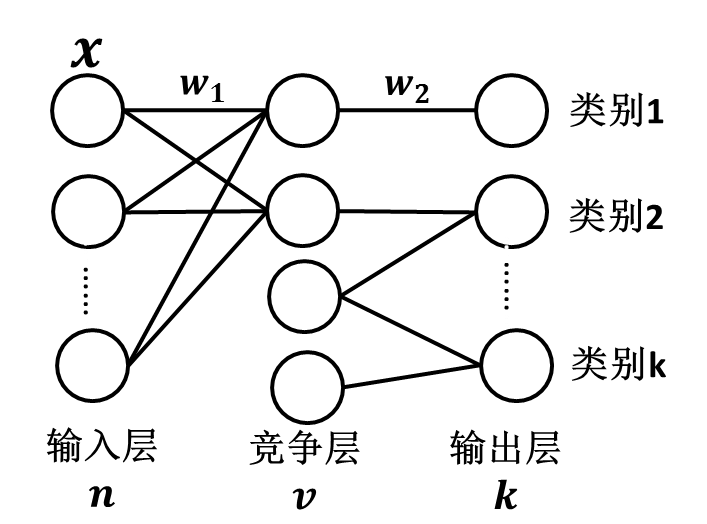
\includegraphics[height=3cm]{images/LVQ_net_sructure.jpg}
            \caption{LVQ网络结构图}
            \label{fig:LVQ网络结构图}
            \end{figure}
        \subsubsection{LVQ学习算法}
            \par
            LVQ的学习算法是:“奖罚”学习算法。具体地,假设在训练样本集内随机选择$D$个\uline{初始模板向量}(初始Veronoi向量),对于来自训练集的任意一个样本$x$,如果$x$与最近的模板属于同一类,则无需学习;否则将惩罚分类错误的模板,奖励其对应正确类别的模板。若经过迭代后,所有向量量化(Veroni向量)不再明显变化,则收敛。
            \par
            例如:某LVQ竞争层有6个神经元,输出层有3个神经元(代表3类)。若竞争层的1、3神经元与第1个输出神经元连接,2、5与第2个输出神经元连接,3、6与第3个神经元连接,则竞争层与输出层的连接权重为
            \begin{align*}
            W_2 =
            \begin{pmatrix}
            1 & 0 & 0\\
            0 & 1 & 0\\
            1 & 0 & 0\\
            0 & 0 & 1\\
            0 & 1 & 0\\
            0 & 0 & 1\\
            \end{pmatrix}
            \end{align*}
            注:$W_2$的行表示输出层3个神经元。我们在训练之前预先设定好$W_2$,从而指定了输出神经元的类别,训练中不再改变。网络的学习通过改变输入层到竞争层权重$W_1$来进行,根据输入样本类别和获胜神经元所属类别可判断当前分类是否正确,若分类正确,则将获胜神经元的权向量向输入向量(样本)方向调整,分了错误则向相反的方向调整。下面给出LVQ学习算法的步骤。
            \par
            LVQ学习算法1:\\
            \textbf{Step1}.初始化。初始化$W_2$且训练过程中不再改变;输入层到竞争层的权重$W_1 = (w_{ij})$;学习率$\eta(0)$,置$t:=0$,$T_{max}$。\\
            \textbf{Step2}.将一个样本$x,x\in R^n$输入到输入层,计算竞争层神经元与输入向量的距离
            \begin{align*}
            d_j = ||x-w_j||\quad j = 1,2,\dots,l
            \end{align*}
            其中:$l$为竞争层神经元个数,$x\in R^n$,$w_j\in R^n$是$W_1$矩阵的第$j$列。\\
            \textbf{Step3}.选取获胜神经元
            \begin{align*}
            j^* = \min _j\{d_j\}
            \end{align*}
            记与$j^*$连接的线性输出层神经元的标签为$c_i$(预测类别)。\\
            \textbf{Step4}.更新权重$W_1$。样本$x$的实际类别为$c_x$,如果$c_i = c_x$,则
            \begin{align*}
            w_{j^*}:=w_{j^*}+\eta(x-w_{j^*})
            \end{align*}
            否则
            \begin{align*}
            w_{j^*}:=w_{j^*}-\eta(x-w_{j^*})
            \end{align*}
            其它非获胜神经元的权重不变。\\
            \textbf{Step5}.更新学习率
            \begin{align*}
            \eta(t) = \eta(0) \left( 1-\frac{t}{T_{max}} \right)
            \end{align*}
            \textbf{Step6}.终止条件。如果不终止,置$t:t+1$返回Step2。
            注:我们在$t$时刻下循环所有样本。
            \par
            LVQ学习算法2。在LVQ学习算法1中,每个样本$x$只会有一个获胜神经元$j^*$,即只有一个神经元更新权重$w_j$。为了提高分类正确率以及算法的收敛速率,Kohonen改进了LVQ1,并称该进后的算法为LVQ2。LVQ2算法基于光滑的移动决策边界逼近Bayes极限。在这之后,LVQ2被修改为LVQ2.1,并进一步有了LVQ3。LVQ2的算法步骤如下:\\
            \textbf{Step1}.利用LVQ1对所有样本进行学习。\\
            \textbf{Step2}.将一样本$x = (x_1,x_2,\dots,x_n)^\mathrm{T}\in R^n$输入到输入层,并计算它与竞争层个神经元之间的距离
            \begin{align*}
            d_j = ||x-w_j||\quad j=1,2,\dots,l
            \end{align*}
            \textbf{Step3}.选择与$x$距离最近的2个竞争层神经元$i,j$。\\
            \textbf{Step4}.如果神经元$i,j$满足以下两个条件:
            \begin{enumerate}
            \item $i,j$对应不同的输出类;
            \item
            \begin{align*}
            \min \left\{ \frac{d_i}{d_j} ,\frac{d_j}{d_i} \right\} > \rho
            \end{align*}
            其中:$\rho = \frac{1-w}{1+w}$,$w\in [0.2,0.5]$。
            \end{enumerate}
            则有\\
            (1)如果$i$对应类别$c_i$与样本$x$的类别$c_x$一致时,有
            \begin{align*}
            w_i :=w_i + \alpha(x-w_i)\\
            w_j :=w_j - \alpha(x-w_j)
            \end{align*}
            (2)如果$j$对应类别$c_j$与输入向量$x$的类别$c_x$一致时,有
            \begin{align*}
            w_i :=w_i - \alpha(x-w_i)\\
            w_j :=w_j + \alpha(x-w_j)
            \end{align*}
            \textbf{Step5}.如果不满足Step4,则只要更新距离最近的神经元权重即可。\\
            \textbf{Step6}.终止条件。如果不终止,置$t:=t+1$,返回Step2。

        \subsubsection{MATLAB应用示例}
            \par
            MATLAB中用lvqnet来实现LVQ网络,其调用格式为
            \par
            lvqnet(hiddenSize,lvqLR,lvqLF)\\
            其中:lvqLR为学习率,默认为0.01;lvqLF为学习函数,默认为'learnlv1'。示例为
            \begin{lstlisting}[language = Matlab]
            [x,y] = iris_dataset;
            net = lvqnet(10);
            net.trainParm.epochs = 50;
            view(net);
            y_hat = net(x);
            pref = perform(net,y_hat,y);
            classes = vec2ind(y_hat)
            \end{lstlisting}
            注:MATLAB中还提供了competlayer和patternnet网络。

    \subsection{对向传播网络CPN}
        \subsubsection{CPN网络结构}
            \par
            对向传播网络CPN(Counter Propagation Network)是将Kononen特征映射网络与Grossberg基本竞争型网络相结合,并它会各自特点的一种特征映射网络。由美国计算机专家Robert Hecht-Nielsen于1987年提出,并广泛用于模式分类、函数逼近、统计方式和数据压缩等领域。
            \par
            CPN网络结构分为3层:输入层、竞争层和输出层。输入层与竞争层构成SOM网络,竞争层与输出层构成基本竞争型网络。从整体上看,网络属于有导师型网络,并结合了SOM无导师的特点,其网络示意图如图(\ref{fig:CPN网络结构图})所示
            \begin{figure}[H]
            \centering
            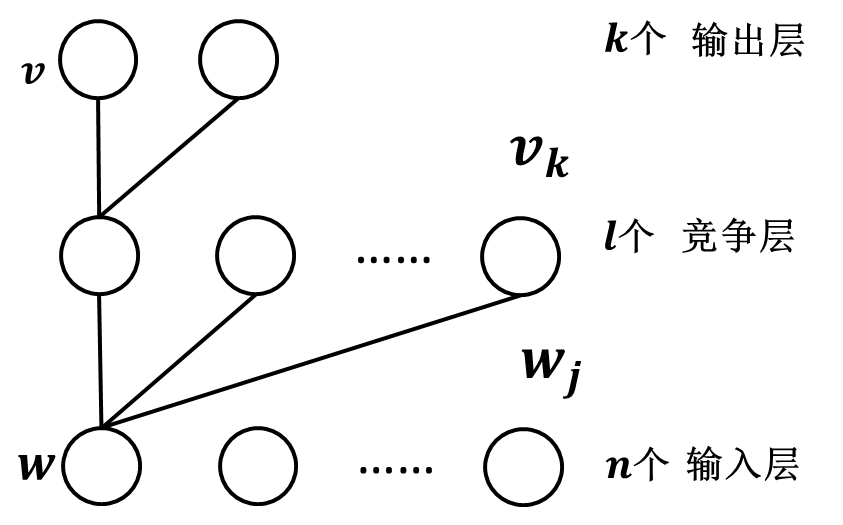
\includegraphics[height=3cm]{images/CPN_net_sructure.png}
            \caption{CPN网络结构图}
            \label{fig:CPN网络结构图}
            \end{figure}
            其中:输入层神经元个数为$n$,共$m$个样本,竞争层有$l$个神经元,其输出为$0,1$,输出层有$K$个神经元(共$K$类),输入层到竞争层权重为$W$,竞争层到输出层权重为$V$。从输出层到竞争层,CPN网络按照SOM学习规则产生获胜神经元,得到各输出神经元的实际输出值,并按照有导师式的误差校正方法修正权重$V$。
        \subsubsection{CPN学习算法}
            \par
            下面,我们给出CPN的学习算法。\\
            \textbf{Step1}.初始化。初始化权重$W,V$,并将样本归一化。\\
            \textbf{Step2}.输入单一样本$x,x\in R^n$到输入层。\\
            \textbf{Step3}.将权重$w_j$归一化
            \begin{align*}
            w_j = \frac{w_j}{||w_j||} \quad j=1,2,\dots,l
            \end{align*}
            \textbf{Step4}.求竞争层中每个神经元$j(j =1,2,\dots,l)$的输入
            \begin{align*}
            S_j = xw_j
            \end{align*}
            \textbf{Step5}.求上千种$\{w_j\}$中与$x$最接近的向量$w_{j^*}$。当$j = j^*$时,记$b_j = 1$,否则记为$b_j=0$。将$j^*$神经元的输出设置为1,其余不变。\\
            \textbf{Step6}.修正$w_{j^*}$
            \begin{align*}
            w_{j^*} := w_{j^*} + \eta(x-w_{j^*})
            \end{align*}
            并将$w_{j^*}$归一化。\\
            \textbf{Step7}.修正$v_k$
            \begin{align*}
            v_k:=v_k + \beta b_j(c_k - c_k') \quad k=1,2,\dots,K
            \end{align*}
            其中:$c_k$为第$k$个输出类别,$c_k'$为真实输出类别。上式可简写为
            \begin{align*}
            v_{j^*k}:=v_{j^*k} + \beta b_j(c_k - c_k')
            \end{align*}
            只需要调整竞争层获胜神经元$j^*$到输出层神经元的连接权向量$v_{j^*}$即可,其余权重不变。\\
            \textbf{Step8}.求输出值
            \begin{align*}
            c_k = bv_k \quad k=1,2,\dots,K
            \end{align*}
            其中:$c\in \{0,1\}^l$。可简写为
            \begin{align*}
            c_k = v_{kj^*}
            \end{align*}
            \textbf{Step9}.返回Step2,直到$m$个样本都输入一遍。\\
            \textbf{Step10}.终止条件。不终止,则置$t:=t+1$,返回Step2。

\section{反馈型神经网络}
    \subsection{Hopfield网络}
        \subsubsection{Hopfield网络的建立}
            \par
            1982年,美国加州理工大学生物物理学家Hopfield提出一种新颖的人工神经网络 - Hopfield网络。Hopfield网络摒弃了神经网络中“层”的概念,创造出全连接神经网络,并且在网络训练时引入Lyapunov函数(能量函数),通过网络训练来使网络的能量最小。这一引入阐明了神经网络与动力学之间的关系,使神经网络的稳定性有了判断依据。Hopfield根据网络输入和输出的不同,可以分为两种类型:离散型Hopfield网络和连续型Hopfield网络。
            \par
            Hopfield最早提出的是离散型二值Hopfield神经网路(DHNN),其神经元的输出只有$1$和$-1$,前面我们谈到的前向型神经网络和竞争型神经网络,它们的网络结构都是前向的,不具有自回归,如图(\ref{fig:反馈网络示意图})所示
   			\begin{figure}[H]
    			\centering
    			\begin{subfigure}[b]{0.2\textwidth}
        			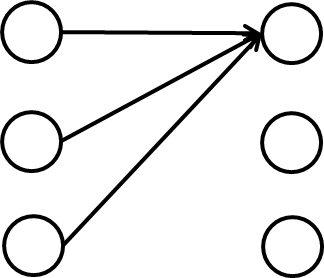
\includegraphics[width=\textwidth]{images/feedback_network1.jpg}
        			\caption{前向型网络}
        			\label{fig:前向型网络}
    			\end{subfigure}
    			\quad
    			\begin{subfigure}[b]{0.2\textwidth}
        			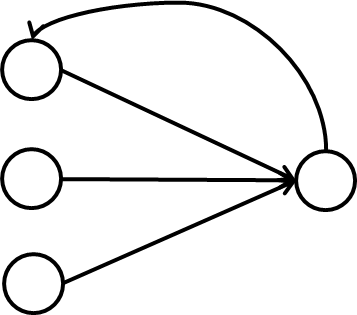
\includegraphics[width=\textwidth]{images/feedback_network2.jpg}
        			\caption{反馈型神经网络1}
        			\label{fig:反馈型神经网络1}
    			\end{subfigure}
    			\quad
    			\begin{subfigure}[b]{0.25\textwidth}
        			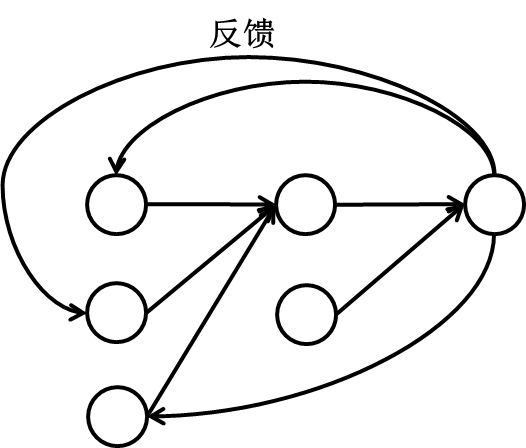
\includegraphics[width=\textwidth]{images/feedback_network3.jpg}
        			\caption{反馈型神经网络2}
        			\label{fig:反馈型神经网络2}
    			\end{subfigure}
    			\caption{反馈网络示意图}\label{fig:反馈网络示意图}
			\end{figure}
            % \textcolor[rgb]{1 0 0}{todo:图片:反馈网络示意图}\\
            如果从图论中图的连接方式来看,前向型网络是图(\ref{fig:反馈网络示意图})中(a)的单向连接,而反馈型神经网络则是图(\ref{fig:反馈网络示意图})中(b)(c)的无向连接或双向连接。
            \par
            为了导出Hopfield网络,我们仍然从分类/回归问题开始:
            \begin{align*}
            \hat{y} = f(w^\mathrm{T}x-\theta)
            \end{align*}
            其中:为了迎合神经网络,我们将$+\theta$写为$-\theta$。现在考虑一个有意思的问题,如果我们令$y=x$呢?有
            \begin{align*}
            \hat{x} = f(w^\mathrm{T}x-\theta)
            \end{align*}
            在系统论中,上述两个模型都是系统,只不过一个是因响应系统,一个是自响应系统。如果设迭代次数(时间)为$t$,则
            \begin{align*}
            x(t+1) = f(w^\mathrm{T}x(t)-\theta)
            \end{align*}
            即$t+1$时刻系统值$x(t+1)$与$t$时刻系统值$x(t)$有关。在微分方程部分,我们研究了这种方程的一些性质,比如:Lyapunov稳定,吸引子等等。
            \par
            假设我们已经有了权重矩阵$W\in R^{n\times n}$,则通过不断的迭代,我们会有系统轨迹$x(0)$,$x(1)$,$\dots$。记$\{x(t)\}^\mathrm{T}$为系统轨迹,平稳是指:当$t\rightarrow \infty$时,$\lim\limits_{t\rightarrow \infty} x(t)\rightarrow x^*$,则称$x^*$为稳定点。我们写出使$x(t)$稳定的过程:\\
            \textbf{Step1}.初始化。初始权重$w_0$,bais $\theta_0$,$x(0)$,置$t:=0$,$T_{max}$。\\
            \textbf{Step2}.计算$x(t+1)$。
            \begin{align*}
            x(t+1) = f(w^\mathrm{T}x(t)-\theta)
            \end{align*}
            \textbf{Step3}.判断是否稳定。
            \begin{align*}
            x(t+1) = x(t)
            \end{align*}
            \textbf{Step4}.终止条件。如果$x(t+1) = x(t)$或者$t = T_{max}$则终止。
            \par
            现在,我们有$m$个样本,每个样本$k$为$x^k = (x_1^k,x_2^k,\dots,x_n^k)\in \{-1,1\}^n$,即共有$n$变量$x_i$,且$n$个变量均为$-1,1$型变量。在给定$w = (w_{ij})_{n\times n}$后,可以写出其关系式
            \begin{align*}
            x = f(w^\mathrm{T}x - \theta)
            \end{align*}
            并且,为了使$x$能够为$\pm 1$,我们设置$f$为sgn,于是有
            \begin{align*}
            x & = f(w^\mathrm{T}x - \theta)\\
            & = \mathrm{sgn}(w^\mathrm{T}x - \theta)
            \end{align*}
            注:我们给定的权重$w = (w_{ij})_{n\times n}$有$w_{ii} = 0$,并且可以设置$w_{ij} = w_{ji}$。
            \par
            将上面的关系式绘制成网络图,如图(\ref{fig:自回归网络图})所示
            \begin{figure}[H]
            \centering
            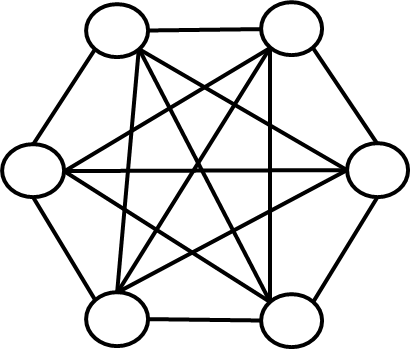
\includegraphics[height=3cm]{images/autoregressive_network.jpg}
            \caption{自回归网络图}
            \label{fig:自回归网络图}
            \end{figure}
            就某个神经元$x_j(j=1,2,\dots,n)$来看,有
            \begin{align*}
            x_j & = f\left(\sum_i w_{ij}x_j -\theta_j\right)\\
            & =\mathrm{sgn}\left(\sum_i w_{ij}x_j -\theta_j\right) =
            \left\{
            \begin{aligned}
            1\\
            -1
            \end{aligned}
            \right.
            \end{align*}
            \par
            在$w,\theta$给定之后,如果给定某个样本$x^k(k = 1,2,\dots,m)$,将$x^k$输入到到网络中,由前面的动力学(微分方程)部分,我们知道$x^k$随着时间$t$的变化会稳定下来:$x^k(0),x^k(1),\dots,x^k(t)\rightarrow x^{k*}$。并且,我们是在$t$时刻将$x^k(t)$整体输入到网络中,并转化为$x^k(t+1)$,现在,我们仅转化样本$x^k$的一个分量$x_j^k$或部分分量,让其余分量不变,以减小计算量和存储量,于是$x^k$有以下收敛步骤:\\
            \textbf{Step1}.初始化。第$k$个样本$x^k(0)$,$w,\theta$,置$t:=0$,$T_{max}$。\\
            \textbf{Step2}.挑选第$j$个变量进行更新
            \begin{align*}
            x_j^k(t+1) = f \left( \sum_iw_{ij}x^k_j -\theta_j \right)
            \end{align*}
            其余变量保持不变
            \begin{align*}
            x_i^k(t+1) = x_i^k(t) \quad i = 1,2,\dots,n,i\neq j
            \end{align*}
            \textbf{Step3}.判断是否稳定
            \begin{align*}
            x^k(t+1) = x^k(t)
            \end{align*}
            \textbf{Step4}.终止条件。若$x^k(t+1) = x^k(t)$或者$t = T_{max}$,则终止;否则,置$t:= t+1$,返回Step2。
        \subsubsection{Hopfield网络的学习算法}
            \par
            上面的收敛过程中,我们假设已经得到了权重$w,\theta$,但是,$w$和$\theta$应该如何获得呢?从网络最初建立时的初始空间状态,到设计适当的连接权重$w$和阈值$\theta$使网络具有知识,具有对给定模式(样本)的联想能力,其中的权重设计过程就是Hopfield网络的学习过程。下面,我们来介绍几种求权重$w$的方法。
            \paragraph{方法1:Hebb外积法}(1)若只有一个样本$x^k(k=1,2,\dots,m)$,对$x^k$而言,若网络达到稳定状态,则有(先忽略$\theta$)
            \begin{align*}
            x^k = \mathrm{sgn}(x^kw)
            \end{align*}
            即
            \begin{align*}
            x_j^k = \mathrm{sgn} \left( \sum_{i=1}^n w_{ij}x_i^k \right) \quad j=1,2,\dots,n
            \end{align*}
            由sgn函数的特点可知,若$x_j^k\left( \sum_{i=1}^n w_{ij}x_i^k \right)>0$,则上式成立。由上述内容可知,网络的连接权重与输入向量的各分量的关系式为
            \begin{align*}
            w_{ij} = \alpha x_j^kx_i^k
            \end{align*}
            其中:$\alpha$为正常数。(2)若有$m$个样本$x^k$,则由归纳法有权重$w_{ij}$的推广公式
            \begin{align*}
            w_{ij}  = \alpha \sum_{k=1}^mx_j^kx_i^k
            \end{align*}
            由$w_{ii} = 0$,所以上式可以写为
            \begin{align*}
            w = \alpha  \sum_{k=1}^m(x^k)^\mathrm{T}x^k - I
            \end{align*}
            由此,可以得到权重$w$的更新迭代公式的规律:一个样本加一次$(x^k)^\mathrm{T}x^k$,于是有
            \begin{align*}
            & w^0 = 0\\
            & w^k = w^{k-1}+(x^k)^\mathrm{T}x^k - I \quad k = 1,2,\dots,m
            \end{align*}
            \par
            从上述连接权重的学习过程可以看出,权重$w$对样本的记忆是累加实现的,每记一个新的样本$x^k$,就更新一个权重$w^k$。但是,就像前面BP算法分析的那样,一次一个样本的更新权重$w$会使$w$“遗忘”前面的样本。事实上,当网络规模$n$达到一定时,要记忆的样本$m$越多,联想时出错的可能就越大。研究表明,对于具有$n$个神经元的Hopfield网络,当$m$超过$0.15n$时,网络的联想记忆就有可能出错,错误结果对应的是能量函数的局部极小点。
            \paragraph{方法2:伪逆法}由Hebb方法可知
            \begin{align*}
            w_{ij} = \sum_{k=1}^mx_i^k(x^\mathrm{T})_j^k
            \end{align*}
            \par
            将内积写成如下形式
            \begin{align*}
            \sum_i (x^\mathrm{T})_i^k x_i^l = x^\mathrm{T}x
            \end{align*}
            则伪逆学习规则用下式求$w$
            \begin{align*}
            w = X(X^\mathrm{T}X)^{-1} = X X^{\dag}
            \end{align*}
            其中:$X$是所有样本数据。我们知道伪逆$X^\dag$是基于最小二乘法的,关于伪逆我们这里做一些简单的说明:当$m\times n$维矩阵$X$不是方阵时,求逆就变成了伪逆,并且当$m>n$,伪逆写为$X^\dag = (X^\mathrm{T}X)^{-1}X^\mathrm{T}$;当$m<n$,则伪逆写为$X^\dag = X^\mathrm{T}(X^\mathrm{T}X)^{-1}$。另外,还可以用SVD和QR等方法求伪逆$X^\dag$。
            \paragraph{方法3:正交化法}MATLAB用函数命令newhp建立Hopfield网络,newhp就是采用SVD方法来求解伪逆矩阵,进而求解权重$w$d的。其计算步骤如下:\\
            \textbf{Step1}.初始化。$X=\{x_1,x_2,\dots,x_m\}$是$m$个样本数据,$x_i\in \{0,1\}^n$,$\tau>-1$,$h$。\\
            \textbf{Step2}.计算$A$。$A = (x_1,-x_m,x_2-x_m,\dots,x_{m-1}-x_m)^\mathrm{T}\in R^{n\times (n-1)}$。\\
            \textbf{Step3}.对$A$进行SVD奇异值分解
            \begin{align*}
            A = USV^\mathrm{T}
            \end{align*}
            其中:MATLAB命令为svd(A),$U,V$为正交矩阵,$U = (u_1,u_2,\dots,u_n),V = (v_1,v_2,\dots,v_{m-1})$,$S$为对角矩阵,
            \begin{math}
            S=
            \left(
            \begin{smallmatrix}
            \Sigma & 0\\
            0&0\\
            \end{smallmatrix}
             \right)
            \end{math}
            ,$\Sigma=\mathrm{diag}(\lambda_1,\lambda_2,\dots,\lambda_k)$,$k$维空间为$n$为空间的子空间,由$k$个独立基组成,$k = \mathrm{rank}(A)$,设$\{u_1,u_2,\dots,u_k\}$为$A$上的正交基,而$\{u_{k+1},u_{k+2},\dots,u_n\}$为$n$维空间的补正交基。\\
            \textbf{Step4}.利用$U$来设计权重。
            \begin{align*}
            & w_m = \sum_{i=1}^ku_iu_i^\mathrm{T}\\
            & w_p = \sum_{i=k+1}^ku_iu_i^\mathrm{T}\\
            & w_t = w_m - \tau w_p
            \end{align*}
            其中:$\tau$为大于$-1$的参数;$w_m,w_p$满足对称条件,因而$w_t$中分量也满足对称条件,这就保证了系统在异步时能够收敛并且不会出现震荡现象。\\
            \textbf{Step5}.构建网络的偏差矩阵
            \begin{align*}
            b_t = x_m - w_tx_m
            \end{align*}
            \textbf{Step6}.计算$w$
            \begin{align*}
            w = \exp(hw_t)
            \end{align*}
            \textbf{Step7}.计算$b$
            \begin{align*}
            b = V\times
            \begin{bmatrix}
            C_1\times I(k) & 0(k,n-k)\\
            0(n-k,k)&C_2\times I(n-k)
            \end{bmatrix}
            \times U^\mathrm{T}\times b_t
            \end{align*}
            其中:$C_1 = \exp(h)^{-1}$,$C_2 = -\frac{\exp(-2xh-1)}{t}$。
        \subsubsection{Hopfield网络的能量函数}
            \par
            Hoplfield运行过程中,网络不断趋于稳定,那么,我们能否用Lyapunov函数来描述这种系统稳定呢?我们定义Hopfield网络的能量函数(Lyapunov函数)为
            \begin{align*}
            E = -\frac{1}{2} \sum_{i=1}^n\sum_{j=1}^n w_{ij}x_ix_j+\sum_{i=1}^n\theta_ix_i
            \end{align*}
            Hopfield网络是一个非线性动力系统,网络状态的变化过程实际上就是一个使能量函数极小化的过程。为了说明能量单调递减,考虑网络中的任意一个神经元$j$
            \begin{align*}
            E_j & = -\frac{1}{2}\sum_{i=1}^n w_{ij}x_ix_j + \theta_jx_j\\
            & =-\frac{1}{2} x_j\sum_{i=1}^n w_{ij}x_i + \theta_j x_j
            \end{align*}
            \par
            $t$时刻到$t+1$时刻,$j$神经元的能量变化为
            \begin{align*}
            \Delta E_j & = E_j(t+1) - E_j(t) \\
            & =-\frac{1}{2} \Delta x_j\sum_{i=1}^nw_{ij}x_i +\Delta x_j\theta_j\\
            & =- \Delta x_j \left( \sum_{i=1}^nw_{ij}x_i - \theta_j \right) +\frac{1}{2}\Delta x_j \sum_{i=1}^n x_i
            \end{align*}
            由于在$t+1$时刻只有神经元$j$调整了状态,并且个神经元不存在自反馈,所以
            \begin{align*}
            \Delta E_j = -\Delta x_j \left( \sum_{i=1}^nw_{ij}x_i - \theta_j \right)
            \end{align*}
            在$t+1$时刻,有
            \begin{enumerate}
            \item 若神经元$j$的状态未变,则$\Delta x_j = 0$,$\Delta E_j =0 $;
            \item 若神经元$j$的状态由$t$时刻的$-1$变为$t+1$时刻的$1$,则$\Delta x_j = 2$,$ \sum_{i=1}^nw_{ij}x_i - \theta_j > 0$,$\Delta E_j <0$;
            \item 若神经元$j$的状态由$t$时刻的$1$变为$t+1$时刻的$-1$,则$\Delta x_j = -2$,$ \sum_{i=1}^nw_{ij}x_i - \theta_j \leqslant 0$,所以$\Delta E_j \leqslant 0$;
            \end{enumerate}
            综上,当神经元$j$的状态改变时,无论变化如何,能量改变量$\Delta E_j \leqslant 0$。由于$j$为任意一个神经元,所以,网络的能量变化量总小于等于0,即
            \begin{align*}
            \Delta E \leqslant 0
            \end{align*}
            由此,Hopfield网络平稳过程是一个能量极小化过程。并且由于能量函数有界,所以网络一定会趋于稳定状态。
        \subsubsection{MATLAB应用示例}
            \par
            MATLAB中使用newhp函数来实现离散型Hopfield网络,其调用格式为
            \par
            net = newhp(T)\\
            其中:T是m个目标向量的$m\times n$矩阵,元素为$\pm 1$;激活函数为satlins(饱和线性函数)。其示例为
            \begin{lstlisting}[language = Matlab]
            T = [1 1 -1 1; -1 1 1 -1;-1 -1 -1 1; 1 1 1 1; -1 -1 1 1];
            net = newhp(T);
            P = {rands(5,4)};
            [Y,Pf,Af] = net({4,50},{},P);
            Y{end}
            \end{lstlisting}

    \subsection{双向联想记忆网络BAM}
        \subsubsection{BAM的网络结构}
            \par
            前面的Hopfield网络是自连接自回归的形式,B.Kosko于1988年提出BAM(Bidirectional Associature Menory)神经网络,可以实现双向联想($x\to y,y\to x$),其网络结构如图(\ref{fig:BAM网络结构图})
            \begin{figure}[H]
            \centering
            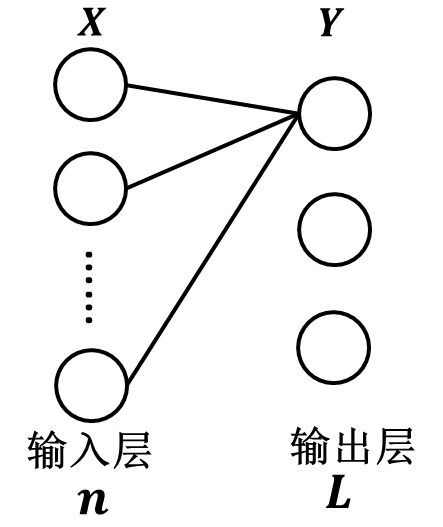
\includegraphics[height=3cm]{images/BAM_network_structure.jpg}
            \caption{BAM网络结构图}
            \label{fig:BAM网络结构图}
            \end{figure}
            BAM的输入层有$n$个神经元,输出层有$l$个神经元,令$X$到$Y$的权重为$W$,则$Y$到$X$的反向权重为$W^\mathrm{T}$。设共有$m$个样本$x^k$,每个样本$x^k$有$n$个输入变量,$x^k = (x_1^k,x_2^k,\dots,x_n^k)\in \{0,1\}^n/\{-1,1\}^n$,有$l$个输出变量$y^k=(y_1^k,y_2^k,\dots,y_l^k)\in \{0,1\}^l/\{-1,1\}^l$。假设我们已经给出了权重$W$,则BAM的运行方式为:将样本$x^k$输入到输入层,有
            \begin{align*}
            y^k = f_y(W x^k)
            \end{align*}
            然后,再将输出$y^k$返回到输入层
            \begin{align*}
            x^k & = f_x(W^\mathrm{T}y^k)\\
            & = f_x \left( W^\mathrm{T}f_y(W x^k) \right)
            \end{align*}
            当$x^k,y^k$的神经元状态不再改变时,网络稳定。由上式我们可以看到$x^k$的更新过程:$t$时刻,网络状态为$x^k(t),y^k(t)$,$t+1$时刻,网络状态为$x^k(t+1) = f_x \left( W^\mathrm{T}f_y(W x^k(t)) \right) ,y^k(t+1) = f_y(W x^k(t))$。
            \par
            为了使网络神经元状态处于$\{\pm 1\}$,令$f_x = f_y = \mathrm{sgn}$,或者$f_x = f_y = \mathrm{satlins}$。上面,我们假设已经给出连接权重$W$,下面,我们就来求解$W$。
        \subsubsection{BAM网络的求解}
            \par
            (1)当网络只需要存储一个样本$(x^k,y^k)$时,若使网络稳定,要满足
            \begin{align}
            \label{BAM网络输出}
            \begin{aligned}
            & \mathrm{sgn}(Wx^k) = y^k\\
            & \mathrm{sgn}(W^\mathrm{T}y^k) = x^k
            \end{aligned}
            \end{align}
            易证明,当$W$是$x^k,y^k$的外积时
            \begin{align*}
            W = y^k x^k\\
            W^\mathrm{T}x^ky^k\mathrm{T}
            \end{align*}
            则(\ref{BAM网络输出})式条件必然成立。
            \par
            (2)当网路要存储$m$个样本$(x^k,y^k)_{k=1}^m$时,由归纳法可得到权重$W$的计算公式
            \begin{align*}
            & W = \sum_{k=1}^my^k(x^k)^\mathrm{T}\\
            & W^\mathrm{T}= \sum_{k=1}^mx^k(y^k)^\mathrm{T}
            \end{align*}
            和Hopfield网络的权重一样,BAM的权重也可以用其它方法求解。
        \subsubsection{BAM网络稳定性}
            \par
            \ding{172}无阈值$\theta$。定义BAM网络的Lyapunov函数(能量函数)为
            \begin{align*}
            E = -\frac{1}{2}X^\mathrm{T}W^\mathrm{T} Y - \frac{1}{2}Y^\mathrm{T}WX
            \end{align*}
            其中:$X,Y$为样本矩阵。由于$Y^\mathrm{T}WX = (Y^\mathrm{T}WX)^\mathrm{T} = (WX)^\mathrm{T}Y = X^\mathrm{T}W^\mathrm{T}Y$,所有$E$也可以写为
            \begin{align}
            \label{BAM网络能量函数}
            E = -X^\mathrm{T}W^\mathrm{T}Y
            \end{align}
            可见,(\ref{BAM网络能量函数})式与Hopfield网络的能量函数相似。由上述内容可知,样本点$(x^k,y^k)$为BAM网络的稳定状态。
            \par
            设$\Delta x$引起的能量变化为$\Delta E_x$
            \begin{align*}
            \Delta E_x = -\Delta X^\mathrm{T}W^\mathrm{T}Y = -\sum_{i=1}^n \Delta x_i \underline{\sum_{j=1}^l w_{ji}y_j}
            \end{align*}
            设$\Delta y$引起的能量变化为$\Delta E_y$
            \begin{align*}
            \Delta E_y = -\Delta Y^\mathrm{T}WX = -\sum_{j=1}^l \Delta y_j \underline{\sum_{i=1}^n w_{ij}x_i}
            \end{align*}
            当$\Delta X \neq 0$时,$\forall \Delta x_i$和$\sum\limits_{j=1}^l w_{ji}y_j$,有$\Delta E_x \leqslant 0$;当$\Delta Y \neq 0$时,$\forall \Delta y_j$和$\sum\limits_{i=1}^l w_{ij}x_i$,有$\Delta E_y \leqslant 0$。所以,当$\Delta X \neq 0,\Delta Y \neq 0$时,$\Delta E \leqslant 0$。\\
            \ding{173}考虑阈值$\theta$。令$\theta_i(i=1,2,\dots,n)$为$x_i$的阈值,$\mu_j(j=1,2,\dots,l)$为$y_j$的阈值,则此时的BAM网络为
            \begin{align*}
            & Y^k(t+1) = f_y(W X^k(t) - \mu)\\
            & X^k(t+1) = f_x(W^\mathrm{T}Y^k(t+1) - \theta) = f_x(W^\mathrm{T}f_y(WX^k(t)-\mu)-\theta)
            \end{align*}
            \par
            定义其Lyaponov函数为
            \begin{align*}
            E = -XWY^\mathrm{T} + X\theta + Y\mu
            \end{align*}
            有能量差为
            \begin{align*}
            \Delta E & = E(t+1) - E(t)\\
            & = -(\Delta X) WY^\mathrm{T}+(\Delta X)\theta^\mathrm{T}\\
            & =-(\Delta X) (WY^\mathrm{T} - \theta^\mathrm{T}) \\
            & = -(\Delta x_i) \left( \sum_{j=1}^l w_{ij}y_+\theta_i \right)
            \end{align*}
            由于$x_i$是双性的,即$x_i\in \{\pm 1\}$,所以$\Delta x_i$必为$\pm 2$或$0$。\ding{172}如果$x_i=0$,则状态有变化,$\Delta E <0$;\ding{173}如果$\Delta x_i = -2$,则$\sum\limits_{j=1}^l y_jw_{ij}-\theta_i <0$,从而$\Delta E < 0$;\ding{174}如果$\Delta x_i=2$,则$\sum\limits_{j=1}^ly_jw_{ij}-\theta_i > 0$,从而$\Delta E < 0$,由此可见,当BAM网络状态改变时,有$\Delta E <0$。

    \subsection{盒中脑BSB}
        \subsubsection{BSB网络结构}
            \par
            盒中脑模型(Brain State in a Box)由Anderson于1977年提出。BSB基本上是一个带幅度限制的正反馈系统,我们仍然使用前面聚类数据$\{x^k\}_{k=1}^m$,$x^k = (x_1^k,x_2^k,\dots,x_n^k)\in R^n$,由此,我们可以想到它的网络结构是:输入层有$n$个神经元,输出层有$n$个神经元;设输入层到输出层的连接权重为$W\in R^{n\times n}$,并且假设$W$是对称矩阵,且$W$的最大特征值为正实数,$\lambda_{max}>0$。BSB的网络结构如图(\ref{fig:BSB的网络结构图})
            \begin{figure}[H]
            \centering
            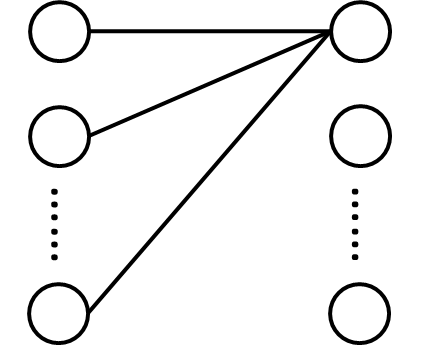
\includegraphics[height=3cm]{images/BSB_network_structure.jpg}
            \caption{BSB网络结构图}
            \label{fig:BSB的网络结构图}
            \end{figure}
            我们仍然假设已经有了$W$,以便观察BSB的运行方式:对于某一个样本$x^k$,将$x^k$输入到网络,有
            \begin{align*}
            y^k = x^k+\beta W x^k
            \end{align*}
            然后,将$y^k$反向传递给输入层,有
            \begin{align*}
            x^k = \varphi(y^k)
            \end{align*}
            其中:$\beta$是一个小常数,$x^k$为$n$维向量,$\varphi$是sgn或者siglins函数。由上面的传递过程,我们可以看出,$x^k$在不同时刻$t$的状态为
            \begin{align*}
            & y^k(t) = x^k(t)+\beta W x^k(t)\\
            & x^k(t+1) = \varphi(y^k(t)) = \varphi(x^k(t)+\beta Wx^k(t))
            \end{align*}
            \par
            直觉上,BSB模型的正反馈环节导致初始状态$x^k(0)$的范数随着迭代次数$t$的增加而增加,直到它撞到盒子(单位超立方体)的壁上,然后顺着壁滑行,最终停在盒子的一个稳定角点上,这也是BSB名字的由来。
        \subsubsection{BSB模型稳定性}
            \par
            我们就输入层某个神经元$j(j=1,2,\dots,n)$来看
            \begin{align*}
            x_j(t+1) = \varphi \left( \sum_{i=1}^n c_{ji}x_i(t) \right)
            \end{align*}
            其中:系数$c_{ji} = \delta_{ji}+\beta_{w_{ji}}$,$\delta_{ji}$为Kronecker delta函数,仅当$j=i$时为1。
            \par
            定义BSB模型的Lyapunov函数如下(1990.Grossberg)
            \begin{align*}
            E = -\frac{\beta}{2} \sum_{i=1}^n\sum_{j=1}^n w_{ji}x_jx_i = -\frac{\beta}{2} X^\mathrm{T} X
            \end{align*}
            Golden在1986年分析了BSB模型,指出:BSB模型实际上是一个梯度下降算法,使能量函数$E$最小,并且,值得一提的是:这要求权重矩阵$W$满足下面2个条件:\ding{172}$W$是对称的;\ding{173}$W$是半正定的,$\lambda_{min} \geqslant 0$。这样,当在时刻$t+1$时,状态向量$x(t+1)$与在时刻$t$的状态向量$x(t)$不同时,BSB模型的能量函数$E$随$t$的增加而减小。更近一步,能量函数$E$的最小点定义了BSB的平衡状态,模型由
            \begin{align*}
            x(t+1) = x(t)
            \end{align*}
            表征,即BSB是一个能量最小化网络。
            \par
            BSB模型的平衡状态由单位超立方体的特定的角点和它的原点定义,在后一种情况,状态向量的任何波动,无论多小,都会被模型的正反馈环节放大,因此导致模型从原点向稳定状态转移。换句话说,原点是一个鞍点。对超立方体来说,要使它的每一个角点作为BSB模型的平衡状态,权重矩阵$W$还要满足第3个条件(1988.Greenberg):\ding{174}权重矩阵$W$是对角有事的(dominant),即
            \begin{align*}
            w_{jj} \geqslant \sum_{i \neq j}|w_{ij}| \quad j= 1,2,\dots,n
            \end{align*}
            \par
            为了使平稳状态$x$稳定,也就是为了使单位超立方体的一个特定角点是一个笃定的吸引子,在单位超立方体中,必须有一个吸引盒$N(x)$,使得对$N(x)$中的所有初始状态向量$x(0)$,BSB都收敛到$x$。为了使单位超立方体的每个角点都可能是一个吸引子,$W$必须满足第4个条件(1988.Greenberg):\ding{175}$W$是强对角优势的,即
            \begin{align*}
            w_{jj} \geqslant \sum_{i \neq j}|w_{ij}|+\alpha \quad j= 1,2,\dots,n
            \end{align*}
            \par
            如果BSB模型的权重$W$只是对称的和半正定的,则单位超立方体中只有一些角点是吸引子,如果$W$还满足条件\ding{174}\ding{175},则单位超立方体中的所有角点都是潜在的吸引子。

    \subsection{极限学习机ELM}
        \par
        无论是在时间序列问题中,还是在微分方程或者是语音(文本)处理当中,时间延迟都起到了至关重要的作用,因为许多情况下,我们说$y$与$x$有关,不仅与$t$时刻的$x$有关(例:$y(t) = f(x(t))$),还与$t-\tau$时刻的$x$有关(例:$y(t) = f(x(t),x(t-\tau))$)。Elman神经网络是J.L.Elman于1990年针对语音处理问题提出来的一种网络,它是一种典型的局部回归网络。Elman网络具有与多层前向网络相似的多层结构,它的主要结构是前向连接,有输入层、隐含层、承接层和输出层4个网络层,输入层隐含层和输出层同BP网络相似,而承接层的作用是:通过连接记忆将上一个时刻的隐含层状态同当前时刻的网络输入一起作为隐含层的输入,相当于状态反馈。隐含层传递函数仍为某种非线性函数,一般为sigmoid函数;输出层的传递函数为线性函数;承接层也为线性函数,其网络结构示意图如图(\ref{fig:ELM网络结构示意图})所示
            \begin{figure}[H]
            \centering
            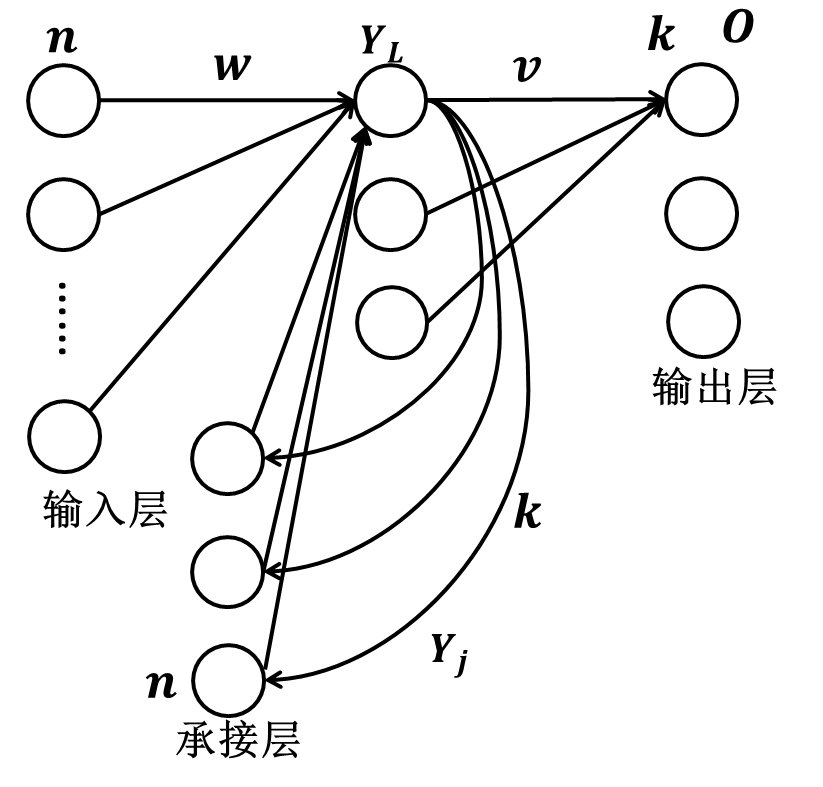
\includegraphics[height=6cm]{images/ELM_network_structure.jpg}
            \caption{ELM网络结构示意图}
            \label{fig:ELM网络结构示意图}
            \end{figure}
        设输入层有$n$个神经元,输出层有$K$个神经元,隐含层有$L$个神经元,承接层有$L$个神经元,输入层到隐含层的权重为$W$,承接层到隐含层的权重为$R$,隐含层到输出层的权重为$V$。我们共有$m$个样本$x^k = (x_1^k,\dots,x_n^k),k=1,2,\dots,m$。
        \par
        仍假设已经有了网络权重$W,R,V$,来研究ELM的运行方式。ELM的运行方式为:将样本$x^k$输入到输入层,隐含层的输入为$W^\mathrm{T}x^k+ R^\mathrm{T}Y_J$,隐含层输出为$Y_L= f_1(W^\mathrm{T}x^k+R^\mathrm{T}Y_J)$,承接层的输入为$Y_L$,承接层的输出为$Y_J = Y_L$,输出层的输出为$o^k = f_2(V^\mathrm{T}Y_L)$。
        \par
        由上面的ELM的运行方式可以看出,ELM网络的权重更新(学习方式)可以用BP算法。以$m$个样本的总离差平方和最小为目标,有
        \begin{align*}
        \min_w \ E = \sum_{k=1}^m E_k & = \frac{1}{2} \sum_{k=1}^m||o^k-y^k||^2\\
        & = \frac{1}{2} \sum_{k=1}^m (e^k)^\mathrm{T}e^k\\
        & =\frac{1}{2} \sum_{k=1}^m \sum_{i=1}^K (o_i^k - y_i^k)^2\\
        & =\frac{1}{2} \sum_{i=1}^K||o_i-y_i||^2
        \end{align*}
        \par
        就像BP算法中那样,无论求$\min E$还是$\min E_k$,我们都用全部样本$X$,所以求解的梯度方向是全局梯度方向,为了加快收敛速度,我们采用SGD或MBGD等方法。对于计算梯度的问题,只需要在BP算法的基础上再求一个$R$权重的梯度即可,这里,我们不再继续讨论了。后面,我们将进入深度学习部分,我们先从BM网络谈起,接着按照$BM\to RBM\to DBN\to DBM$的顺序进行。
        \par
        MATLAB中使用elmannet函数来实现ELM网络,其调用格式为
        \par
        elmannet(layerdelays,hiddenSizes,trainFcn)\\
        其中:layerdelays是延迟数,默认为1:2。

    \subsection{玻尔兹曼机BM}
        \subsubsection{BM简介}
            \par
            深度学习模型DBN和DBM是由限制玻尔兹曼机RBM堆积而成的,而RBM是在玻尔兹曼机BM的基础上进行改进的,为此,我们先来讨论一下BM。并且,由于深度学习发展速度非常快,基本上每天都有新内容,所以DBN和DBM可能已经被淘汰掉了。关于深度学习模型,我们只介绍一些有里程碑意义的模型。
            \par
            模拟退火算法是1953年N.Metropolis等人在研究二维相变时提出的。1983年,S.Kirkpatrzck等用模拟退火设计大规模集成电路(VLSI)。G.E.Hinton、TJ.Sepjmowski和D.H.Ackley等于1983年,借助统计力学的概念和方法,把模拟退火方法引入到Hopfield网络中,使Hopfield有了随机性,从而提出了玻尔兹曼机。1984年S.Geman和D.Geman给出退火率$T \propto 1/\log t$,但这个退火过程太慢,因而效率很低,几乎没有太大使用价值。1985年,Harold Szu提出了一种快速模拟退火法,称为柯西机(Cauchy Machine),这使得BM方法有了应用的可能。从前面优化部分介绍的模拟退火来看,它相对于普通的爬山法而言,具有随机性,有一定概率跳出局部极小点,因此,模拟退火法可以看成是“随机梯度下降法”。
            \par
            前面提到的BP网络和Hopfield网络用的梯度方向都是使目标函数下降的梯度方向,由于\ding{172}网络中存在输入到输出的非线性映射,从而使网络的误差或能量函数是含有许多极小点的非线性超平面,即非凸;\ding{173}在算法上,只能按目标函数梯度减小的方向变化,这导致BP和Hopfield很有可能陷入局部极小点。为此,我们可以在算法中引入随机梯度方向来克服这一缺陷。随机型神经网络有以下特点:
            \begin{enumerate}
            \item 各神经元的输入不能决定其输出状态是0或者1,而是决定了输出为0或者1的概率;
            \item 在网络学习阶段,随机型神经网络并不基于某种确定性算法调整网络连接权值,而是按照某种概率分布进行处理;
            \item 在网络运行阶段,随机型神经网络不是按照某种确定性的网络方程进行状态改变,而是按照某种概率分布决定网络状态的转移。
            \end{enumerate}
        \subsubsection{BM的网络结构}
            \par
            BM的网络结构和Hopfield网络的结构相似,网络中的$n$个神经元之间相互连接,为双向连接结构,且每个神经元到自身无反馈$w_{ii} = 0$。我们可以假设$w_{ij} = w_{ji}(i,j=1,2,\dots,n)$。每个神经元的输出$x_j$均为0或1,其网络结构如图(\ref{fig:BM网络结构示意图})所示
			\begin{figure}[H]
  			\centering
  			\begin{varwidth}[t]{\textwidth}
    			\vspace{0pt}
    			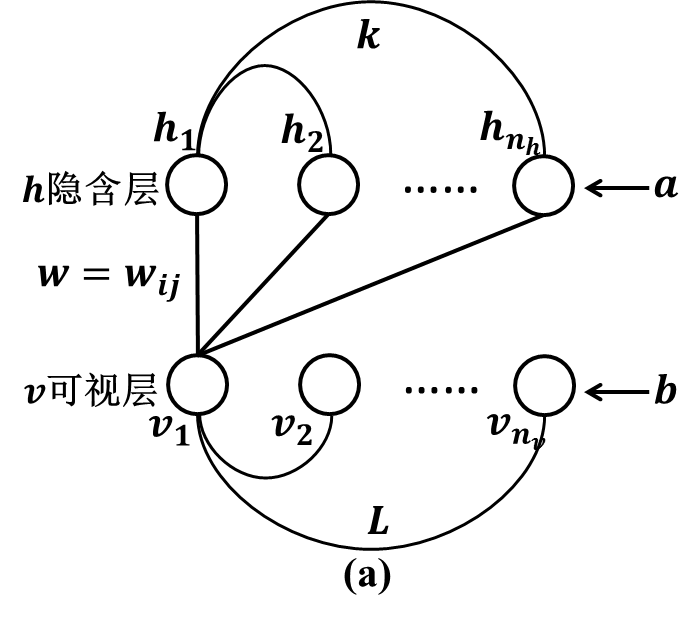
\includegraphics[height=4cm]{images/BM_network_structure1.jpg}
  			\end{varwidth}
  			\qquad
  			\begin{varwidth}[t]{\textwidth}
    			\vspace{0pt}
    			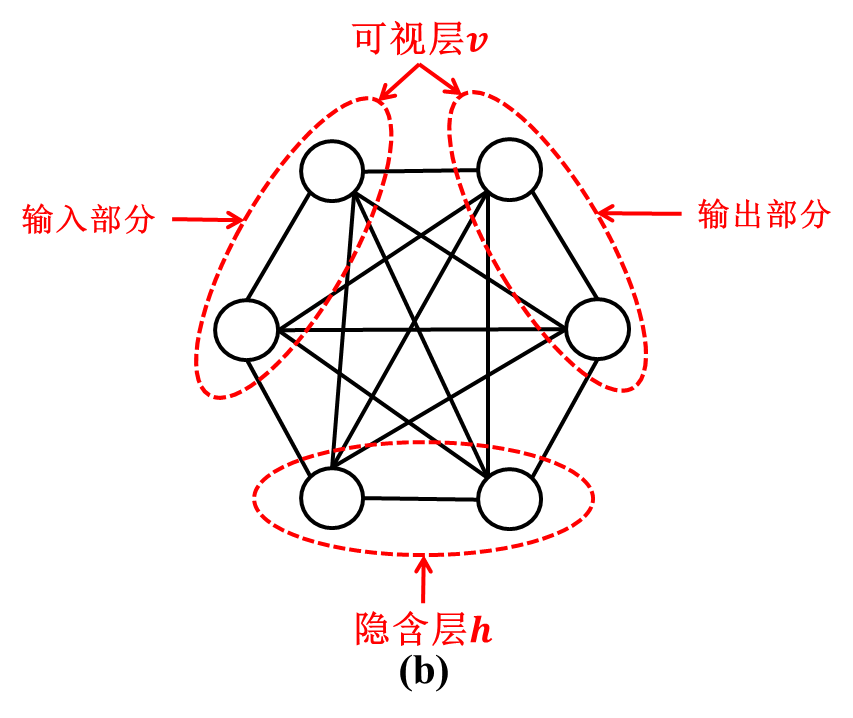
\includegraphics[height=4.5cm]{images/BM_network_structure2.jpg}
  			\end{varwidth}
            \caption{BM网络结构示意图}
            \label{fig:BM网络结构示意图}
            \end{figure}
            注:输入层加上输出层为可视层,对自己学习(自联想)无输出层,而互联想,有输出层。如果不考虑层次结构,网络结构如图(\ref{fig:BM网络结构示意图})(b)所示,共有$n$个神经元,在$t$时刻,网络的状态为$X(t) = (x_1,x_2,\dots,x_n)$。如果考虑层次结构,可将BM分为可视层$v$和隐含层$h$,设可视层(visiable)神经元个数为$n_v$,隐含层(hidden)神经元个数为$n_h$,则有$n = n_v+n_h$。隐含层和可视层神经元状态$v_j,h_i$的状态值为0或1。这里所说的$v_j,h_i$即为$x_j$。值得一提的是:与Hopfield网络不同的是,这里的$v_i,h_j$或者$x_j$的状态值为随机变量,其输出值$\sum_i w_{ij}x_i - \theta_j$只是$x_j$取值为0或1的概率,而不是具体的神经元状态,即
            \begin{align*}
            P(x_j = 1) = \sum_i w_{ij}x_i - \theta_j
            \end{align*}
            \par
            设$v = (v_1,v_2,\dots,v_{n_v})^\mathrm{T} \in \{0,1\}^{n_v}$为可视层状态向量,是一随机向量,取值为0或1;$h = (h_1,h_2,\dots,h_{n_h})^\mathrm{T} \in \{0,1\}^{n_h}$为隐含层状态向量,是一随机向量,取值为0或1;$a = (a_1,a_2,\dots,a_{n_h})^\mathrm{T}$为隐含层偏置向量(阈值/bias),$a_i\in R$;$b = (b_1,b_2,\dots,b_{n_h})^\mathrm{T}$为可视层偏置向量(阈值/bias),$b_j\in R$;神经元$v_i$和$h_j$的连接权重为$W_{ij}$,则$W = (W_{ij})_{n_v\times n_h}\in R^{n_v\times n_h}$\footnote{注:$x \triangleq (v,h)$,$\theta \triangleq W \triangleq (W,R,L,a,b)$。};神经元$v_i$与$v_j$的连接权重为$L_{ij}$,则$L = (L_{ij})_{n_v\times n_v}\in R^{n_v\times n_v}$;神经元$h_i$与$h_j$的连接权重为$R_{ij}$,则$R = (R_{ij})_{n_h\times n_h}\in R^{n_h\times n_h}$,且注意:各神经元自身不连接,权重为0。
            \par
            上面,给出了BM的网络结构,下面,来看一下BM的网络输出。在Hopfield网络中,神经元$j$的输出为
            \begin{align*}
            x_j = \mathrm{sgn} \left( \sum_{i} w_{ij}x_i - \theta_j \right)  =
            \left\{
            \begin{aligned}
            0\\
            1
            \end{aligned}
            \right.
            \end{align*}
            \par
            但上面说到BM的神经元输出值不再是一变量,而是一个随机变量。所以,我们只能给出神经元$j$取值为1的概率。那么,神经元$j$取值为1的概率是多少呢?或者说我们如何依据输出值$\sum_{i} w_{ij}x_i - \theta_j $来设定其概率呢?(概率求和需要为1),可以借助下面的函数图(\ref{fig:BM神经元概率值示意图})进行说明
            \begin{figure}[H]
            \centering
            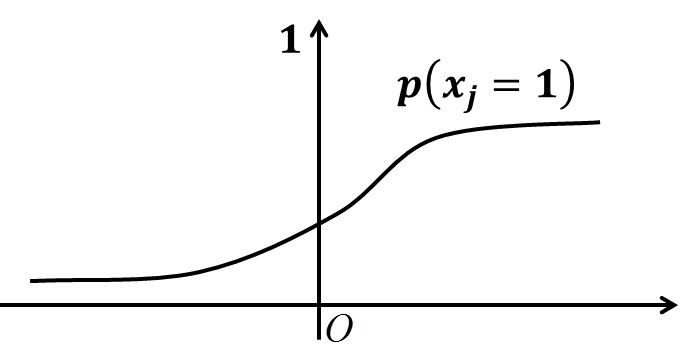
\includegraphics[height=3cm]{images/BM_neuron_probability_values.jpg}
            \caption{BM神经元概率值示意图}
            \label{fig:BM神经元概率值示意图}
            \end{figure}
            神经元$j$取值为1的概率为
            \begin{align*}
            P(x_j = 1) = \frac{1}{1+e^{-s_j/T}} = \frac{1}{1+e^{-\left( \sum_{i} w_{ij}x_i - \theta_j \right) /T}}
            \end{align*}
            神经元$j$取值为0的概率为
            \begin{align*}
            P(x_j = 0) = 1-P(x_j = 1) = \frac{e^{-s_j/T}}{1+e^{-s_j/T}} = \frac{1}{1+e^{s_j/T}}
            \end{align*}
            其中:$T$为温度参数。可以看出,如果神经元$j$的输出$s_j$为0,则$P(x_j=1) = P(x_j=0) = 0.5$,且$s_j$越大,$P(x_j=1)$越大。并且,网络参数$T$会对产生影响:温度$T$越高曲线越平滑,$P(x_j=1)$相对于$s_j$的变化越小,因此,即使神经元$j$的输出$s_j$有较大的变化,也不会对$P(x_j=1)$产生很大的影响。并且,当$T\rightarrow \infty$时,曲线变为一条恒为0.5的直线,$P(x_j=0)=P(x_j=1)$,也就意味着网络中各神经元有更多机会进行状态选择;相反,当$T$越小时,$P(x_j=1)$对$s_j$变化越敏感,即$s_j$的一个小变化,$P(x_j=1)$也会有很大变化,且当$T\rightarrow -\infty$时,概率为1,BM网络也就变为了Hopfield网络。
            \par
            上面,给出了BM网络的输出,下面,我们应该讨论的是:1.BM网络整体取某一状态的概率(联合概率密度),即$X = (x_1,x_2,\dots x_n)^\mathrm{T}$的概率$P(X =(x_1,x_2,\dots x_n)) $;2.BM网络的运行规则;3.BM网络的能量函数;4.BM网络的学习方法,即权重$\theta \triangleq W \triangleq (W,R,L,a,b)$的求解。

        \subsubsection{BM网络的运行规则}
            \par
            假设我们已经得到了参数$\theta \triangleq W \triangleq (W,R,L,a,b)$,BM网络的运行规则和Hopfield网络相似,问题是:\ding{172}如何确定网络已经稳定?\ding{173}异步工作还是同步工作?即$t$时刻改变几个神经元的状态?异步工作是改变一个或部分神经元的状态,同步工作是改变所有神经元的状态。对某个样本$x^k(k=1,2,\dots,m)$而言,将$x^k$输入到BM网络中,其异步运行规则如下:\\
            \textbf{Step1}.初始化。初始温度$T(t=0) = T_0$,终止温度$T_{min}$,参数$\theta=W=(W,R,L,a,b)$。\\
            \textbf{Step2}.在$t$时刻,在温度$T(t) = T_k$下,从网络中随机挑选一个神经元$j(j=1,2,\dots,n)$,计算其输出
            \begin{align*}
            s_j = \sum_{i} w_{ij}x_i - \theta_j
            \end{align*}
            计算神经元$j$的概率值
            \begin{align*}
            P(x_j=1) = \frac{1}{1+e^{-s_j /T_k}}
            \end{align*}
            \textbf{Step3}.更新网络状态。对第$j$个神经元,按上述概率随机更新神经元$j$的状态,得到$x_j(t+1)$;其余神经元的状态不变,即
            \begin{align*}
            x_i(t+1) = x_i(t)\quad i=1,2,\dots,n ,i\neq j
            \end{align*}
            \textbf{Step4}.判断网络在温度$T_k$下是否达到平衡状态,如果未平衡,则转到Step2,否则,转到Step5。\\
            \textbf{Step5}.终止条件。不终止,则置$t:=t+1$,并设置此时的温度$T(t+1) < T(t)$,转到Step2。\\
            注:降温函数可以使用
            \begin{align*}
            & T(t)/T_0 \propto 1/\ln t\\
            & T(t)/T_0 \propto 1/t
            \end{align*}
            即
            \begin{align*}
            & T(t+1) = T_0/\log (t+1)\\
            & T(t+1) = T_0/(t+1)\\
            & T(t+1) = \lambda T(t)
            \end{align*}

        \subsubsection{BM网络的能量函数}
            \par
            与Hopfield相同,我们也采用能量函数来描述网络状态。定义BM网络的能量函数为
            \begin{align*}
            E_\theta(x) = x^\mathrm{T}Wx + \theta^\mathrm{T}x
            \end{align*}
            如果是$v$和$h$,则写为
            \begin{align*}
            E_\theta(v,h) = -v^\mathrm{T}Wh- \frac{1}{2} v^\mathrm{T}L v - \frac{1}{2} h^\mathrm{T} R h- v^\mathrm{T}b- h^\mathrm{T}a
            \end{align*}
            \par
            由
            \begin{align*}
            E = -\frac{1}{2} \sum_{i=1}^n\sum_{j=1}^n w_{ij}x_ix_j +\sum_{i=1}\theta_i x_i
            \end{align*}
            可知,单一神经元$x_j$的能量$E_j$为
            \begin{align*}
            E_j & = -\frac{1}{2}\sum_{i=1}^n w_{ij}x_ix_j+\theta_jx_j\\
            & =-\frac{1}{2} x_j\sum_{i=1}^n w_{ij}x_i + \theta_j x_j
            \end{align*}
            则$t$时刻到$t+1$时刻的能量变化为
            \begin{align*}
            \Delta E_j & = E_j(t+1) - E_j(t) \\
            & =-\frac{1}{2} [x_j(t+1) - x_j(t)] \sum_{i=1}^n w_{ij} x_i + [x_j(t+1) - x_j(t)]\theta_j\\
            & =-\frac{1}{2}\Delta x_j \sum_{i=1}^nw_{ij} x_i + \Delta x_j \theta_j\\
            & = -\Delta x_j \left( \sum_{i=1}^nw_{ij}x_i - \theta_j \right) + \frac{1}{2}\Delta x_j \sum_{i=1}^nw_{ij}x_i
            \end{align*}
            \par
            假设BM采用异步操作方式,即每时刻$t$只有一个神经元$j$的状态可能改变,其余神经元状态不变,则上式$\Delta E_j$可以简写为
            \begin{align*}
            \Delta E_j = -\Delta x_j \left( \sum_{i=1}^n w_{ij}x_i -\theta_j \right) = -\Delta x_js_j
            \end{align*}
            为了分析$\Delta E_j$的大小,在$t+1$时刻,考虑如下三种情况:
            \begin{enumerate}
                \item 若$s_j = 0$,则$\Delta E_j = 0$;
                \item 若$s_j >0$,则$P(x_j=1) > 0.5$,即神经元$j$取值为1的概率较大。此时可以得到以下结论:
                    \begin{enumerate}
                    \item 若$x_j(t)=1$,则$\Delta x_j =0$的概率较大,因此,$\Delta E_j = 0$的概率较大;
                    \item 若$x_j(t)=0$,则$\Delta x_j =1$的概率较大,因此,$\Delta E_j < 0$的概率较大.
                    \end{enumerate}
                \item 若$s_j <0$,则$P(x_j=1)<0.5$,即神经元$j$输出为0的概率较大,此时可得到以下结论:
                    \begin{enumerate}
                    \item 若$x_j(t)=1$,则$\Delta x_j =0$的概率较大,因此,$\Delta E_j = 0$的概率较大;
                    \item 若$x_j(t)=0$,则$\Delta x_j =1$的概率较大,因此,$\Delta E_j < 0$的概率较大.
                    \end{enumerate}
            \end{enumerate}
            \par
            综上可知,当神经元$j$的状态改变时,其能量函数的变化量$\Delta E_j \leqslant 0$的概率较大。由于神经元是任意一个神经元,所以网络全局能量的变化来给你$\Delta E \leqslant 0$的概率也较大。与Hopfield网络不同的是:Hopfield是确定能使能量下降(简单看成目标函数),而BM网络只是可能使能量函数下降,因此,BM具有跳出局部极小点的能力。
        \subsubsection{Boltzmann分布}
            \par
            从前面的Hopfield网络中,我们知道,将一个样本$x^k$输入网络后,随着时间$t$的不断迭代,网络最终会收敛到收敛态,称为$x^k*$,也称$x^k*$为Hopfield对$x^k$的记忆,当然,我们会要求$x^k*$和$x^k$尽可能接近。
            \par
            现在,在BM网络中,我们仍然会有$x^k$和$x^k*$,只不过二者都不再是确定变量,而是随机变量。也就是说,现在要求得$\theta$,使$x^k,x^k*$的概率分布尽可能接近。或者从所有样本来说,我们求使样本出现概率最大的$\theta$,即$\max_\theta P(x^1,x^2,\dots,x^m)$,其中:$x^i$为某一样本。在BM以及后面的RBM中,我们也可能将$m$个样本$\{x^k\}_{k=1}^m$写为$v,h$的形式$\{v^k\}_{k=1}^m$。
            \par
            上面所说的只是对无监督学习而言,如果对于有监督学习,我们可以使$n_h = n_y$,然后用$P(h^1,h^2,\dots,h^{m})$表示输出样本$y$的概率。下面,我们先来求出某一样本$x^k$出现的概率,之后再求其联合概率分布。样本$x^k$出现的概率即为BM网络处于某一状态的概率,例如:$P(x_1 = 1,x_2=0,\dots,x_n=0)$。
            \par
            假设BM在$t$时刻的状态为$X_1\in R^n$,$t+1$时刻的状态为$X_2$,并且BM采用异步运行方式,那么有\\
            (1)如果在$t$时刻,神经元$j$的状态$x_j$为1,设此时的能量函数值为$E(X_1)$;在$t+1$时刻,神经元$j$的状态$x_j$为0,此时的能量函数值为$E(X_2)$,那么
            \begin{align*}
            \Delta E = E(X_2) - E(X_1)= -\Delta x_j s_j = - (0-1)s_j = s_j
            \end{align*}
            有
            \begin{align*}
            & P(x_j = 1)  = \frac{1}{1+e^{-\Delta E/T}}\\
            & P(x_j = 0) = 1-P(x_j = 1)  = \frac{e^{-\Delta E/T}}{1+e^{-\Delta E/T}}
            \end{align*}
            从而
            \begin{align*}
            \frac{P(x_j = 0)}{P(x_j = 1)} = e^{-\Delta E/T} = \frac{e^{- E(X_2)/T}}{e^{- E(X_1)/T}}
            \end{align*}
            由于网络异步运行,因此有
            \begin{align*}
            \frac{P(X_2)}{P(X_1)} = \frac{e^{- E(X_2)/T}}{e^{- E(X_1)/T}}
            \end{align*}
            (2)如果在$t$时刻神经元$j$的状态$x_j$为0,能量为$E(X_1)$,在$t+1$时刻$x_j$为1,能量为$E(X_2)$,那么
            \begin{align*}
            \Delta E = E(X_2)  - E(X_1) = -(1-0)s_j = -s_j
            \end{align*}
            有
            \begin{align*}
            & P(x_j = 1)  = \frac{1}{1+e^{\Delta E/T}}\\
            & P(x_j = 0) = 1-P(x_j = 1)  = \frac{e^{\Delta E/T}}{1+e^{\Delta E/T}}
            \end{align*}
            从而
            \begin{align*}
            \frac{P(x_j = 0)}{P(x_j = 1)} = \frac{e^{- E(X_2)/T}}{e^{- E(X_1)/T}}
            \end{align*}
            由于网络异步运行,因此有
            \begin{align*}
            \frac{P(X_1)}{P(X_2)} = \frac{e^{- E(X_1)/T}}{e^{- E(X_2)/T}}
            \end{align*}
            \par
            由上述(1)(2)可知,BM的任意两个状态$X_1,X_2$出现的概率$P(X_1),P(X_2)$与其能量之间存在一定的关系:某个网络状态对应的能量越低,该状态出现的概率就越大。
            \par
            事实上,统计力学的相关研究表明:在温度$T$,分子停留在状态$x$的概率满足Boltzmann概率分布
            \begin{align*}
            P(E = E(x)) = \frac{e^{-E(x)/T\cdot RH}}{Z(T)}
            \end{align*}
            其中:$E(x)$表示状态$x$时的能量,$RH>0$为玻尔兹曼常数,$E$表示分子能量的一个随机变量,$Z(T)$为概率分布的标准化因子(归一化因子),忽略$RH$,有
            \begin{align*}
            Z(T) = \sum_{x\in D} e^{-E(x)}
            \end{align*}
            $D$为状态$x$的可能取值空间,空间大小为$2^n$或者$2^{n_v\times n_h}$。
            \par
            上面的状态概率分布$P(E = E(x))$可以记为
            \begin{align*}
            P_\theta(v,h) = P(v,h|\theta) = P(v,h;\theta) = P_\theta(x) = \frac{1}{Z(T)}e^{-E_\theta(v,h)}
            \end{align*}
            从中可以看出,能量$E(x)$越大,则状态$x$的概率值越小。为书写简便,我们默认已经给出网络参数$\theta$,所以$P_\theta(v,h) = P(v,h)$。
        \subsubsection{BM学习方法}
            \par
            上面,我们给出了BM网络“输出”某一状态$x^k$的概率,即样本概率,并且,在前面的BM运行规则和能量函数以及状态概率中都假设已经知道了BM网络的权重和偏置等参数$\theta \triangleq W \triangleq (W,R,L,a,b)$。下面,我们就要来讨论如何求解参数$\theta \triangleq W \triangleq (W,R,L,a,b)$。
            \par
            我们知道,对于某一个样本$x^k$而言,其本身有一个概率$P(x^k = x)$,而将$x^k$输入到BM网络后,又有一个概率,我们自然要在这两个概率上做文章,比如:要求BM网络(概率分布)来逼近(近似)样本的真实分布,甚至还可以从BM中生成样本。
            \par
            设共有$m$个样本$\{x^k\}_{k=1}^m$,或者写为$v,h$的形式$\{v^k\}_{k=1}^m$,记样本集为$D_m = \{v^k\}_{k=1}^m$,每个样本$v^k\in \{0,1\}^{n_v}$,例如:样本1经过\underline{01编码}后是$n_v$长度的$v^1 = (0,1\dots,1,0)$;样本2经过\underline{01编码}后是$n_v$长度的$v^2 = (1,1\dots,1,1)$。并且,假设各样本独立同分布。下面介绍两种求解参数的方法:1. K-L距离最小法(交叉熵最小);2.样本概率最大(极大似然估计法)。
            \paragraph{方法1:K-L距离最小法}Hinton最初开发BM网络时,就是采用的K-L最小方法,原文为:能量函数和样本概率分布为
            \begin{align*}
            & E_\theta(v,h) = -v^\mathrm{T}Wh - \frac{1}{2} v^\mathrm{T}Lv - \frac{1}{2}h^\mathrm{T}Rh\\
            & P(v) = \frac{1}{Z_\theta}\sum_h \exp(-E_\theta(v,h) )
            \end{align*}
            其中:$Z_\theta = \sum_v\sum_h \exp(-E_\theta(v,h))$。某一神经元的概率为
            \begin{align*}
            & p(h_j=1|\theta,h_{\cdot j}) = g \left( \sum_i W_{ij}v_i+ \sum_{m\neq j}R_{jm}h_{\cdot,m} \right) \\
            & p(v_i=1|h,v_{\cdot i}) = g \left( \sum_j W_{ij}h_j+ \sum_{k\neq i}L_{ik}v_{k} \right)
            \end{align*}
            权重更新公式为
            \begin{align*}
            & \Delta W = \alpha \left( \mathbb{E}_{P_{data}}[vh^\mathrm{T}]  - \mathbb{E}_{P_{model}}[vh^\mathrm{T}] \right)\\
            & \Delta L = \alpha \left( \mathbb{E}_{P_{data}}[vv^\mathrm{T}]  - \mathbb{E}_{P_{model}}[vv^\mathrm{T}] \right)\\
            & \Delta R = \alpha \left( \mathbb{E}_{P_{data}}[hh^\mathrm{T}]  - \mathbb{E}_{P_{model}}[hh^\mathrm{T}] \right)
            \end{align*}
            其中:
            \begin{align*}
            & P_{data}(v,h) = P_{data}(v)P_{data}(h|v)\\
            & P_{data}(v) = \frac{1}{m} \sum_{k=1}^m\delta (v-v^k)
            \end{align*}
            \par
            下面,来对上面的公式进行说明。不考虑偏置bias,仅就权重$\theta\triangleq (W,R,L)$来看,对某一个样本$v^k$而言
            \begin{align*}
            p^+(v^k,h^l) = \frac{e^{-E_\theta(v^k,h^l)/T}}{Z_\theta}
            \end{align*}
            边缘分布$p(v^k)$写为
            \begin{align*}
            p^+(v^k) = \sum_{h^l}p^+(v^k,h^l) = \frac{1}{Z_\theta}e^{-E_\theta (v^k,h^l)/T}
            \end{align*}
            其中:$v^k\in \{0,1\}^{n_v}$是样本,$h^l\in \{0,1\}^{n_h}$是长度为$n_h$的任意的01值向量($h$如何确定呢?);$p^+$表示$P_{data}$,称$p^+(v^k)$为样本的实际概率。简单理解:样本实际概率就和频数一样,只不过这里有了具体的“频数”计算公式。如果我们给出了$h$的所有可能(或者说$h^l$已知),那么,我们只需要将样本$v^k(k=1,2,\dots,m)$带入上面的计算公式即可(不是带入到BM模型中)。
            \par
            将$v^k$输入到BM模型中,记由模型生成的概率为$p^{-}(v^k)$,即为$P_{model}$。我们要求$p^+(v^k)$和$p^-(v^k)$尽可能接近,用KL距离来衡量两个概率分布之间的接近程度,有
            \begin{align*}
            G(\theta) = \sum_{k=1}^m p^+(v^k) \ln \frac{p^+(v^k)}{p^-(v^k)} = \sum_{k=1}^m p^-(v^k)\ln \frac{p^-(v^k)}{p^+(v^k)}
            \end{align*}
            其中:$G(\theta) \geqslant 0$,并且,只有在$p^+(v^k) = p^-(v^k)$时,$G(\theta) = 0$。显然$G$越小,实际概率(样本概率)$p^+(v^k)$越接近期望概率(模型输出概率)$p^-(v^k)$。因此,BM模型学习的过程就是使$G$达到最小的过程。
            \par
            当然,要注意的是,上面使$G(\theta)$最小的过程是在所有样本$D_m$上进行的,而不是像SGD那样一次一个样本$v^k$。对于$G(\theta)$,我们已经有了$p^+(v^k)$($p^+(v^k)$来源于数据集而非模型,就像数据自身的频率或者经验密度经验分布那样),下面来看$p^-(v^k)$。将$v^k$输入到BM网络后,在网络运行时有
            \begin{align*}
            p^-(v^k) = \sum_{h^l}p(v^k,h^l) = \frac{1}{Z_\theta} e^{-E(v^k,h^l)/T}
            \end{align*}
            下面,将$G(\theta)$关于$\theta\triangleq (W,R,L)$求导,有
            \begin{align*}
            \frac{\partial G}{\partial W_{ij}} = -\sum_k \frac{p^+(v^k)}{p^-(v^k)}\frac{\partial p^-(v^k)}{\partial W_{ij}}
            \end{align*}
            而对$p^-(v^k)$,有
            \begin{align*}
            \frac{\partial p^-(v^k)}{\partial W_{ij}} = \frac{1}{T} \left[ \sum_h p^-(v^k,h^l)s_i^{k,l} s_j^{k,l} - p^-(v^k)\sum_{\lambda,\mu}p^-(v^\lambda,h^\mu)s_i^{\lambda,\mu}s_j^{\lambda,\mu} \right]
            \end{align*}
            其中:$s_i^{\alpha,\beta}$为第$i$个神经元的状态值;$s_j^{\alpha,\beta}$为第$j$个神经元的状态值,且
            \begin{align*}
            \frac{\partial e^{-E(v^\alpha,h^\beta)/T}}{\partial W_{ij}} = \frac{1}{T}s_i^{\alpha,\beta}s_j^{\alpha,\beta}e^{-E(v^\alpha,h^\beta)/T}
            \end{align*}
            于是有
            \begin{align*}
            \frac{\partial G}{\partial W_{ij}} = -\frac{1}{T} \sum_{k} \frac{p^+(v^k)}{p^-(v^k)}\left[ \sum_{h^l} p^-(v^k,h^l)s_i^{k,l} s_j^{k,l} - p^-(v^k)\sum_{\lambda,\mu}p^-(v^\lambda,h^\mu)s_i^{\lambda,\mu}s_j^{\lambda,\mu} \right]
            \end{align*}
            由于
            \begin{align*}
            & p^+(v^k,h^l) = p^+(h^l|v^k)p^+(v^k)\\
            & p^-(v^k,h^l) = p^-(h^l|v^k)p^-(v^k)\\
            & p^+(h^l|v^k) = p^-(h^l|v^k)
            \end{align*}
            所以有
            \begin{align}
            \label{KL求导用到的公式1}
            p^-(v^k,h^l)\frac{p^+(v^k)}{p^-(v^k)} = p^+(v^k,h^l)
            \end{align}
            并且,由于
            \begin{align}
            \label{KL求导用到的公式2}
            \sum_kp^+(v^k) = 1
            \end{align}
            将上式(\ref{KL求导用到的公式1})和式(\ref{KL求导用到的公式2})带入到$\frac{\partial G}{\partial W_{ij}}$,有
            \begin{align*}
            \frac{\partial G}{\partial W_{ij}} & = -\frac{1}{T}\left( \sum_{k}\sum_{h^l}p^+(v^k,h^l) s_i^{k,l} s_j^{k,l} - \sum_{\lambda}\sum_{\mu}p^-(v^\lambda,h^\mu)s_i^{\lambda,\mu}s_j^{\lambda,\mu}\right) \\
            & =-\frac{1}{T} \left( \rho_{ij}^+ - \rho_{ij}^- \right)
            \end{align*}
            其中:$\rho_{ij}^+$是样本中两个神经元$i,j$都处于$1$的平均概率;$\rho_{ij}^-$是网络运行中两个神经元$i,j$都处于$1$的平均概率。
            \par
            最小化$G$的步骤是:当网络处于$T$温度下的热平衡时($v^k$的平稳输出$v^k*$已经形成),观察$\rho_{ij}^+,\rho_{ij}^-$,计算权重更新方向
            \begin{align*}
            \Delta W_{ij} = \frac{\eta}{T}(\rho_{ij}^+ - \rho_{ij}^-)
            \end{align*}
            并更新权重
            \begin{align*}
            W_{ij}:= W_{ij} + \Delta W_{ij}
            \end{align*}
            其中:$\eta$为学习率。更新公式中的$\frac{\eta}{T}\rho_{ij}^+$表示连接权重的调整量$\Delta W_{ij}$与$\rho_{ij}^+$成正比,即$s_i$与$s_j$同时为1的数量越大,$\rho_{ij}^+$越大,$\Delta W_{ij}$越大,称$\frac{\eta}{T}\rho_{ij}^+$为正学习项;相反的,称$\frac{\eta}{T}\rho_{ij}^-$为反学习项。下面,我们给出BM的算法步骤:\\
            \textbf{Step1}.初始化。
            \par
            初始权重$W=(W_{ij})_{n\times n},W_{ij}\in [-1,1],W_{ij} = W_{ji}$。初始温度$T_0$,终止温度$T_{end}$,样本数据集$D_m = \{v^k\}_{k=1}^m$,网络更新次数(Gibbs采样数)$d$,循环次数$t,t_{max}$,学习率$\eta$,由样本集$D_m$计算样本概率$p^+(v^k)$,并令$p^-(v^k) = 0,k=1,2,\dots,m$。\\
            \textbf{Step2}.将某一样本$v^k(k=1,2,\dots,m)$输入到BM可视层。\\
            \textbf{Step3}.从初始温度$T_0$开始,按照BM运行规则,将网络状态$v^k$更新至终止温度$T_{end}$,并输出平衡状态$h^l*$。注:$T(t) = \frac{T_0}{1+\ln t}$或者$T(t) = \frac{T_0}{\log (t+1)}$。 \\
            \textbf{Step4}.在隐含层的平衡状态$h^l*$下,保持温度$T= T_{end}$不变,对整个网络状态进行$d$次更新(一旦达到平衡态,就可以采样2个神经元为1的概率),每次更新后,当神经元$i$与$j$同时为1时,计算
            \begin{align*}
            Count_{ij}^+ = Count_{ij}^+ +1
            \end{align*}
            \textbf{Step5}.重新从初始温度$T_0$开始,按照BM运行规则,将\underline{整个网络}(这里没有输入样本)的状态更新至终止温度$T_{end}$下的平衡态$v^k*,k=1,2,\dots,m$。\\
            \textbf{Step6}.在网络平衡状态下,保持$T= T_{end}$不变,对整个网络继续进行$d$次更新(采样),每次更新当神经元$i,j$同时为1时,计算
            \begin{align*}
            Count_{ij}^- = Count_{ij}^-+1
            \end{align*}
            \textbf{Step7}.返回Step2,直到进行$t$次循环,并且,$t>n_v$。\\
            \textbf{Step8}.按下式计算$\rho_{ij}^+,\rho_{ij}^-(i,j=1,2,\dots,n)$
            \begin{align*}
            \rho_{ij}^+ = \frac{1}{td} Count_{tj}^+\\
            \rho_{ij}^- = \frac{1}{td} Count_{ij}^-
            \end{align*}
            \textbf{Step9}.更新权重。
            \begin{align*}
            W_{ij}:=W_{ij} + \Delta W_{ij} = W_{ij} + \frac{\eta}{T_{end}}(\rho_{ij}^+ - \rho_{ij}^-)
            \end{align*}
            \textbf{Step10}.返回Step2,直至进行$t_{max}$次循环。
            \par
            下面,我们再给出一个更详细的步骤:\\
            \textbf{Step1}.初始化。
            \par
            初始权重$W=(W_{ij})_{n\times n},W_{ij}\in [-1,1],W_{ij} = W_{ji}$。初始温度$T_0$,终止温度$T_{end}$,样本数据集$D_m = \{v^k\}_{k=1}^m$,网络更新次数(Gibbs采样数/Markov链长)$d$,循环次数$t,t_{max}$,学习率$\eta$,由样本集$D_m$计算样本概率$p^+(v^k)$,并令$p^-(v^k) = 0,k=1,2,\dots,m$,容许误差$\varepsilon$。\\
            \textbf{Step2}.\textbf{正阶段}:对于一个样本$v^k,k=1,2,\dots,m$,将其输入到BM网络,并随机设置其隐含层神经元状态$h^k$(当然,如果是有标签样本的话,$h^k$设置为标签状态)。注意:这里的$h^k$随机开始要让其达到稳定是耗时的,不如有指导性的设置。\\
            \ding{172}在温度$T$下,使网络达到平衡;\\
            \ding{173}置$t:=1$,挑选隐含层节点$j(j=1,2,\dots,n_h)$,将其状态翻转
            \begin{align*}
            h_j=
            \left\{
            \begin{aligned}
            1\quad h_j(t-1) = 0\\
            0\quad h_j(t-1) = 1
            \end{aligned}
            \right.
            \end{align*}
            其余神经元状态不变。\\
            \ding{174}计算翻转后的网络能量变化
            \begin{align*}
            & E(t-1) = v^\mathrm{T}Wh(t-1)\\
            & E(t) = v^\mathrm{T}Wh(t)\\
            & \Delta E_j = E(t)-E(t-1)
            \end{align*}
            \ding{175}判断神经元$j$的状态是否改变。如果$\Delta E_j<0$,则状态改变;否则$\Delta E_j \geqslant 0$,计算概率$P_j = e^{-\Delta E_j/T(t)}$,如果$P_j >\lambda$,则接受新状态,否则状态不变。\\
            \ding{176}如果隐含层节点为完全考察(未遍历),或者状态未稳定,则返回\ding{173};否则转到\ding{177}。当在温度$T$下稳定时,才进入下一温度。\\
            \ding{177}终止条件。若$T(t) \leqslant T_{end}$则终止;否则,令$t:=t+1$,计算温度$T(t) = \frac{T_0}{1+\ln t}$或者$T(t) = \frac{T_0}{\log (t+1)}$。
            \textbf{Step3}.记录平衡时隐含层神经元状态$h^l*$。\\
            \textbf{Step4}.在隐含层的平衡状态$h^l*$下,保持温度$T= T_{end}$不变,对整个网络状态进行$d$次更新(一旦达到平衡态,就可以采样2个神经元为1的概率),每次更新后,当神经元$i$与$j$同时为1时,计算
            \begin{align*}
            Count_{ij}^+ = Count_{ij}^+ +1
            \end{align*}
            \textbf{Step5}.选取新样本$v^k$,返回Step2。在遍历所有样本后,计算可视层神经元$v_i$和隐含层神经元$h_j$状态同时为1的频率$\rho_{ij}^+$
            \begin{align*}
            \rho_{ij}^+ = \frac{1}{td} Count_{ij}^+ \quad i,j =1,2,\dots,n
            \end{align*}
            注:仔细观察$td$,可以知道吉布斯采样的由来,以及$\sum_h$的求解。\\
            \textbf{Step6}.\textbf{负阶段}:对虚拟样本$v^k$(这里的样本数量可以是$m$也可以不是),随机设置可视层$v$和隐含层$h$的初始状态(随机2值)。置$t:=1$,更新$v,h$的状态,直到网络平衡为止。输出网络平衡态$v^k*,h^l*$。\\
            \textbf{Step7}.在隐含层的平衡状态$h^l*$下,保持温度$T= T_{end}$不变,对整个网络状态进行$d$次更新(一旦达到平衡态,就可以采样2个神经元为1的概率),每次更新后,当神经元$i$与$j$同时为1时,计算
            \begin{align*}
            Count_{ij}^- = Count_{ij}^- +1
            \end{align*}
            \textbf{Step8}.选取新样本$v^k$,返回Step6。直到遍历所有样本。注意:这里的Step2和Step6可以合并。计算可视层神经元$v_i$和隐含层神经元$h_j$状态相同的频率$\rho_{ij}^-$
            \begin{align*}
            \rho_{ij}^- = \frac{1}{td}Count_{ij}^-
            \end{align*}
            \textbf{Step9}.调整权重
            \begin{align*}
            W_{ij} := W_{ij} +\Delta W_{ij} = W_{ij} + \frac{\eta}{T}(\rho_{ij}^+-\rho_{ij}^-)
            \end{align*}
            \textbf{Step10}.返回Step2,直到$\Delta W_{ij}<\varepsilon$,即$\rho_{ij}^+ = \rho{ij}^-$相接近时。\\
            注:1.$\rho_{ij}^+ = \big < v_i,h_j\big >_{data}^+ = \sum\sum p(h,v)v_ih_j$;2.$d$过程即为Gibbs采样过程。

            \paragraph{方法2:极大似然估计法} 上面求解参数$W$的方法是基于最小化K-L距离的,下面介绍参数的极大似然估计。当前,我们已经讨论过了:把样本$v^k(k=1,2,\dots,m)$输入到BM网络中,当网络稳定时,会得到其概率
            \begin{align*}
            p^-(v^k) = \sum_{h^l}p^-(v^k,h^l) = \frac{1}{Z_\theta} \sum_{h^l}e^{-E(v^k,h^l)}
            \end{align*}
            现在,我们要求$\theta$,使样本出现的(联合)概率最大
            \begin{align*}
            \max_\theta\ L(\theta) = P(v^1,v^2,\dots,v^m) = \prod_{k=1}^mp(v^k)
            \end{align*}
            由于$\max L$与$\max \ln L$是等价的,有
            \begin{align*}
            \max_\theta \ \ln L(\theta)=\log\prod_{k=1}^mp(v^k) = \sum_{k=1}^m\log p(v^k)
            \end{align*}
            将上式关于$\theta$求导,有
            \begin{align*}
            \frac{\partial \ln L(\theta)}{\partial \theta} = \sum_{k=1}^m \frac{\partial \ln p(v^k)}{\partial \theta}
            \end{align*}
            所以,我们先来处理单一样本$v^k$的导数。这里的$p(v^k)$可以记为$p_\theta(v^k),p(v^k|\theta)$或者$p(v^k;\theta)$。下面就来处理$\frac{\partial \ln p(v^k)}{\partial \theta}$,由边缘分布,有
            \begin{align*}
            \ln p(v^k) & = \ln \sum_h p(v^k,h)\\
            & =\ln \frac{1}{Z} \sum_h e^{-E(v^k,h)}\\
            & =\ln \sum_he^{-E(v^k,h)} -\ln Z
            \end{align*}
            有
            \begin{align*}
            &\frac{\partial \ln p(v^k)}{\partial \theta}\\
            ={}& \frac{\partial }{\partial \theta} \left( \ln \sum_he^{-E(v^k,h)} \right)  - \frac{\partial }{\partial \theta} \ln Z\\
            ={}&-\frac{1}{\sum_he^{-E(v^k,h)}}\sum_he^{-E(v^k,h)}\frac{\partial E(v^k,h)}{\partial \theta} + \frac{1}{\sum_{v,h} e^{-E(v,h)}}\sum_{v,h} e^{-E(v,h)}\frac{\partial E(v,h)}{\partial \theta}\\
            ={}&-\sum_h\frac{e^{-E(v^k,h)}}{\sum_he^{-E(v^k,h)}}\frac{\partial E(v^k,h)}{\partial \theta} + \sum_{v,h}p(v,h)\frac{\partial E(v,h)}{\partial \theta}\\
            ={}&-\sum_h\frac{\frac{e^{-E(v^k,h)}}{Z}}{\frac{\sum_he^{-E(v^k,h)}}{Z}}\frac{\partial E(v^k,h)}{\partial \theta} + \sum_{v,h}p(v,h)\frac{\partial E(v,h)}{\partial \theta}\\
            ={}&- \sum_h \frac{e^{-E(v^k,h)}}{\sum_h\frac{e^{-E(v^k,h)}}{Z}}\frac{\partial E(v^k,h)}{\partial \theta} + \sum_{v,h}p(v,h)\frac{\partial E(v,h)}{\partial \theta}\\
            ={}& -\sum_h \frac{p(v^k,h)}{p(v^k)}\frac{\partial E(v^k,h)}{\partial \theta} + \sum_{v,h}p(v,h)\frac{\partial E(v,h)}{\partial \theta}\\
            ={}& - \sum_h p(h|v^k)\frac{\partial E(v^k,h)}{\partial \theta} + \sum_{v,h}p(v,h)\frac{\partial E(v,h)}{\partial \theta}
            \end{align*}
            即
            \begin{align}
            \label{BM极大似然估计梯度}
            \frac{\partial \ln p(v^k)}{\partial \theta} & = -\sum_h p(h|v^k)\frac{\partial E(v^k,h)}{\partial \theta} + \sum_{v,h}p(v,h)\frac{\partial E(v,h)}{\partial \theta} \\
            & =- \mathbb{E}_{p(h|v^k)} \left[ \frac{\partial E(v^k,h)}{\partial \theta} \right] + \mathbb{E}_{p(v,h)} \left[ \frac{\partial E(v,h)}{\partial \theta}  \right]\notag\\
            & =-\Big<\frac{\partial E(v^k,h)}{\partial \theta}  \Big>_{p(h|v^k)} + \Big<\frac{\partial E(v,h)}{\partial \theta}  \Big>_{p(v,h)} \notag
            \end{align}
            \par
            这里,用极大似然求解的梯度与KL距离求解的梯度一致,就像前面的BM学习算法中描述的那样:$p(h|v^k)$部分是我们从样本$v^k$出发,求解的$h$的状态;而$p(h,v)$部分是随机出发,求出的整个网络$v,h$的状态。我们将其改写为
            \begin{align*}
            & \mathbb{E}_{p(h|v^k)} \left[ \frac{\partial E(v^k,h)}{\partial \theta} \right] = \rho_{ij}^+\\
            & \mathbb{E}_{p(v,h)} \left[ \frac{\partial E(v,h)}{\partial \theta}  \right] = \rho_{ij}^-
            \end{align*}
            \par
            我们先来看
            \begin{align*}
            \frac{\partial E(v,h)}{\partial \theta}
            \end{align*}
            上式的取值取决于能量函数$E(v,h)$的形式。一般而言,$E(v,h)$有以下几种形式
            \begin{align*}
            & E(v,h) = -v^\mathrm{T}Wh - \frac{1}{2}v^\mathrm{T}Lv - \frac{1}{2}h^\mathrm{T}Rh - v^\mathrm{T}b-h^\mathrm{T}a\\
            & E(v,h) = -v^\mathrm{T}Wh - \frac{1}{2}v^\mathrm{T}Lv - \frac{1}{2}h^\mathrm{T}Rh\\
            & E(v,h) = -v^\mathrm{T}Wh - v^\mathrm{T}b-h^\mathrm{T}a \quad \text{限制玻尔兹曼机}\\
            & E(v,h) = -v^\mathrm{T}Wh - \frac{1}{2}v^\mathrm{T}Lv - v^\mathrm{T}b-h^\mathrm{T}a\quad\text{半限制玻尔兹曼机}
            \end{align*}
            前面,我们说过不讨论阈值$a,b$,所以,这里采用第二种$E(v,h)$,它的导数为
            \begin{align*}
            & \frac{\partial E}{\partial W} = vh^\mathrm{T}\\
            & \frac{\partial E}{\partial L} = vv^\mathrm{T}\\
            & \frac{\partial E}{\partial R} = hh^\mathrm{T}
            \end{align*}
            \par
            下面来讨论(\ref{BM极大似然估计梯度})式中等式右边的第二项
            \begin{align*}
            &\sum_{v,h}p(v,h) \frac{\partial E(v,h)}{\partial \theta}\\
            = {}&\sum_v\sum_h p(v)p(h|v)\frac{\partial E}{\partial \theta}\\
            = {}&\sum_vp(v)\sum_hp(h|v)\frac{\partial E}{\partial \theta}
            \end{align*}
            因此,只要知道$\sum_hp(h|v)$即可。其中:$p(h|v)$是隐含层神经元$h = (h_1,h_2,\dots,h_{n_h})$的条件联合概率分布,我们自然会想:联合概率分布是否为各边缘分布的乘积?
            \begin{align*}
            p(h|v) = \prod_{j=1}^{n_h}p(h_j|v)
            \end{align*}
            可惜的是,只有在各随机变量(隐含层神经元)相互独立的时候,联合概率才等于各概率的乘积,也就是如果隐含层$h$神经元之间不存在互连接($h_i,h_j$无关),则上式成立。为了使用上式,我们可以构建如下图(\ref{fig:RBM网络结构图1})的限制玻尔兹曼机RBM,这个留在后面介绍。
            \begin{figure}[H]
            \centering
            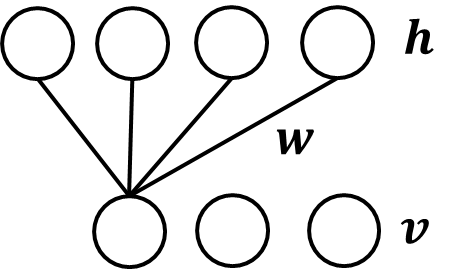
\includegraphics[width=4cm]{images/RBM_net_structure1.jpg}
            \caption{RBM网络结构图}
            \label{fig:RBM网络结构图1}
            \end{figure}
            % \textcolor[rgb]{1 0 0}{todo:图片:RBM网络结构图1}
            \par
            回到我们的问题当中,第一个数据期望$\langle\cdot\rangle_{data}$是易求的,$\langle\cdot\rangle_{data}$是$v_i,h_j$同时取1的概率;而$\langle\cdot\rangle_{model}$是以最终模型(稳定时的模型)定义的分布来求的,当隐含层神经元未知时,$\langle\cdot\rangle_{model}$要花费指数时间来精确计算,我们不得不寻找其近似方法。
            \par
            典型BM学习方法主要有:吉布斯采样(Gibbs sampleing)、平行回火(paralled tem-pering)、变分近似法(Variational approach)、随机近似法(stochastic approximation procedure, SAP)、对比散度算法(contrastive divergence, KCD)、持续对比散度(persistant contrastive dirergance, PCD)和快速持续对比散度(fast persistent contrastive dirergence, FPCD)。
            \paragraph{Gibbs sampling}就是前面在BM学习算法中用到的方法。吉布斯采样法是马尔科夫链算法的一种,给定一个$n$维随机向量$x=(x_1,x_2,x_n)$,无法求得$x$的联合概率分布$p(x)$,但是知道给定$x$的部分分量后,$x_i$的条件概率分布$p(x_i|x_{-i})$,其中:$x_{-i}$表示$x$中不含$x_i$的部分。可以从$x$的任意状态(即样本状态)开始,利用条件分布$p(x_i|x_{-i})$迭代并对其分量依次采样。随着采样次数的增加,随机变量$x_1(k),x_2(k),\dots,x_n(k)$的概率分布将以$k$的几何级数的速度收敛于$x$的联合概率分布$p(x)$。在BM的每个迭代过程中,设置一个马尔科夫链,并将其运行到平衡状态,用马尔科夫链近似期望值$\mathbb{E}_{P_{model}}[\cdot]$。这个算法的优点是通用性较好,缺点是计算量较高,运行缓慢,在每次迭代过程中都要等到每个马尔科夫链达到平稳分布(平稳状态)。
            \paragraph{随机近似SAP}1992.Neal\cite{1992.Neal}提出一种新的BM训练算法。在前面的BM学习算法步骤中,我们曾提到过,$h$从一个随机状态开始,要花费很长时间才能达到热平衡,那么为什么不给一个近似平稳的状态呢?例如:我们可以选用上一个样本的平衡作为开始。我们称这种预先存储好的近似平衡的状态为particle(粒子,是一个向量),可以在正负阶段使用粒子,在正阶段,会夹逼出一个数据向量,而负阶段就不需要夹逼任何东西。
            \par
            SAP方法属于广义Robbins-Monro式随机近似法,用于近似期望值$\mathbb{E}_{P_{model}}[\cdot]$。SAP学习过程可行的主要原因是:当学习率$\eta$相对于马尔科夫链的混合速率变得足够小时,持续马尔科夫链将会一直接近平稳分布,对于成功的参数更新,从持续马尔科夫链采集的数据将会高度关联。
            \par
            给定一个独立同分布的样本集$D_m = \{x^k\}_{k=1}^N$,考虑含有充分统计量的样本分布
            \begin{align*}
            p(x|\theta) = \frac{1}{Z_\theta} \exp(\theta^\mathrm{T}\phi(x))
            \end{align*}
            上式取对数,并关于$\theta$求导,有
            \begin{align*}
            \frac{\partial \log p(\theta|x)}{\partial \theta} = \frac{1}{N}\sum_{n=1}^N\phi(x^n) - \mathbb{E}_{P_{model}}[\phi(x)] = S(\theta)
            \end{align*}
            假设$\theta^t$和$\tilde{x}^t$是当前时刻的参数和状态,则$\theta^t,\tilde{ x}^t$按下列算法(\ref{code:SAP算法})更新。
             \begin{algorithm}[h]
                \caption{A Stochastic Approximation Procedure for Estimating the BM(SAP)}\label{code:SAP算法}
                \begin{algorithmic}[1]
                    \State Give a data set $D_m = \{x^k\}_{k=1}^N$; Randomly initialize $\theta$ and $M$ sample particles $X^{0,M}=\{\tilde{ x}^{0,1},\dots,\tilde{x}^{0,M}\}$
                    \For{$t = 0:T$(number of interations) }
                        \For{$i=1:M$(number of parallel Markov chains) }
                            \State Sample $\tilde{ x}^{t+1,i}$ ,given $\tilde{x}^{t,i}$ using transition operator $T_t(\tilde{ x}^{t+1,i} \leftarrow \tilde{ x}^{t,i})$
                        \EndFor
                        \State update
                        \begin{align*}
                        \theta^{t+1} & =\theta^t + \alpha_t \left[ \frac{1}{N}\sum_{n=1}^N\phi(x^n) - \frac{1}{M}\sum_{m=1}^M\phi(\tilde{x}^{t+1,m})  \right]\\
                        & =\theta^t + \alpha_t S(\theta_t) + \alpha_t \left[\mathbb{E}_{P_{model}}[\phi(x)] - \frac{1}{M}\sum_{m=1}^M\phi(\tilde{ x}^{t+1,m})\right]\\
                        & =\theta^t + \alpha_t S(\theta^t)+\alpha^t\epsilon_{t+1}
                        \end{align*}
                        注:ensure almost sure envergence to aon as $y$mptotically stable point of $\dot{\theta} = S(\theta)$, require $\sum_{t=0}^\infty \alpha_t = \infty,\sum_{t=0}^\infty \alpha_t^2 < \infty$.
                        \State Decrease $\alpha_t$
                    \EndFor
                \end{algorithmic}
            \end{algorithm}
            其中:用点估计$\phi(\tilde{x}^{t+1})$来估计$\mathbb{E}_{P_{model}}[\phi(x)]$。

            \paragraph{变分推断}在变分学习中,对每个训练样本可视层向量$v$,用近似后验分布$q(h|v,\mu)$替换隐单元向量上的真实后验分布$p(h|v,\theta)$。BM模型的对数似然函数有下面形式的变分下界
            \begin{align*}
            \ln p(v,\theta) & \geqslant \sum_j q(h_j|v,\mu)\ln p(v,h,\theta) + H(q)\\
            & =\ln p(v,\theta) - \mathrm{KL}(q(h|v,\mu)||p(v|h,\theta))
            \end{align*}
            其中:$H(\cdot)$为熵。变分近似法能够很好的估计$\mathbb{E}_{P_{data}}[\cdot]$,而不能用于估计$\mathbb{E}_{P_{model}}[\cdot]$。变分近似法的伪代码如下(\ref{code:Variational 算法})
             \begin{algorithm}[htbp]
                \caption{A Variational Approach for Estimating the BM(SAP)}\label{code:Variational 算法}
                \begin{algorithmic}[1]
                    \State Given: a data set $D_m = \{v^k\}_{k=1}^N$; Randomly initialize $\theta$ and $M$ sample particles $\{\tilde{ v}^{0,1},\tilde{h}^{0,1}\},\dots,\{\tilde{ v}^{0,M},\tilde{h}^{0,M}\}$。
                    \For{$t = 0:T$(number of interations) }
                        \State $//$ variational inference(变分推断:正阶段)\cite{1999.Jorden.M}
                        \For { each training example $v^n,n=1,2,\dots,N$  }
                            \State Randomly initialine $\mu$ and run mean - field updates(\underline{平均场}) until convergence
                            \State $\mu_j \leftarrow g(\sum_i W_{ij}v_i + \sum_{m\neq j}R_{mj}\mu_m)$
                            \State Set $\mu^n = \mu$
                        \EndFor
                        \State $//$ Stochastic Appkroximation(随机近似:负阶段)
                        \For {each sample $m=1:M$(number of persistent Markov Chains) }
                            \State Sample $(\tilde{v}^{t+1,m},\tilde{h}^{t+1,m})$, given $(\tilde{v}^{t,m},\tilde{h}^{,m})$ by using a Gibbs sample in
                            \begin{align*}
                            & p(h_j=1|v,h_{-j}) = g\left(\sum_iW_{ij}v_i + \sum_{m\neq j}R_{jm}h_m\right)\\
                            & p(v_i=1|h,v_{-i}) = g\left(\sum_jW_{ij}h_j + \sum_{k\neq i}L_{ik}v_k\right)
                            \end{align*}
                        \EndFor
                        \State $//$ Parameter update
                        \begin{align*}
                        & W^{t+1} \leftarrow W^t + \alpha_t \left( \frac{1}{N}\sum_{n=1}^Nv^n (\mu^n)^\mathrm{T} - \frac{1}{M} \sum_{m=1}^M \tilde{v}^{t+1,m} (h^{t+1,m})^\mathrm{T}\right)\\
                        & R^{t+1} \leftarrow R^t + \alpha_t \left( \frac{1}{N} \mu^n(\mu^n)^\mathrm{T} - \frac{1}{M} \sum_{m=1}^M h^{t+1,m} (h^{t+1,m})^\mathrm{T} \right)\\
                        & L^{t+1} \leftarrow L^t + \alpha_t \left( \frac{1}{N} v^n(v^n)^\mathrm{T} - \frac{1}{M} \sum_{m=1}^M \tilde{v}^{t+1,m} (\tilde{v}^{t+1,m})^\mathrm{T} \right)
                        \end{align*}
                        \State Decrease $\alpha_t$
                    \EndFor
                \end{algorithmic}
            \end{algorithm}
            \par
            Neal的方法在全批量上是适用的,而在mini batch上比较困难,因为我们用到了同样的数据向量,会使得权重更新有很多相同。所以,针对数据向量而存储的粒子将不再是在热平衡(平衡态)附近了。假设当一个数据向量$v$被夹逼的时候,这些好的解释(也就是隐含层状态)扮演着那个数据向量的解释是单峰的,即对于一个数据向量$v$,没有2个不同的解释$h$。基于此,我们简记一下平均场逼近法:\\
            (1)如果我们想得到正确统计数据,需要随机循环来更新神经元状态
            \begin{align*}
            p_i = p(s_i = 1) = \sigma\left(b_i + \sum_j s_j W_{ij}\right)
            \end{align*}
            (2)如果我们不打算保持$i$的二值状态(我们说神经元$i$是随机的,值仅有0和1),而保持一个实值状态,可以用
            \begin{align*}
            p_i^{t+1} = \sigma\left(b_i + \sum_j p_j^t W_{ij}\right)
            \end{align*}
            用一个概率实值来代替原来的随机二值,但这样并不是很好,因为随机二值是在非线性函数内部的。如果是一条线性函数,那没事。但因为是sigmoid非线性函数,每当我们替代时,就得不到正确答案。\\
            (3)为了解决biphasic oscillations, 我们采用damped mean field(和动量moment相似)
            \begin{align*}
            p_i^{t+1} = \lambda p_i^t + (1-\lambda)\sigma\left(b_i + \sum_j p_j^t W_{ij}\right)
            \end{align*}

    \subsection{限制玻尔兹曼机RBM}
        \subsubsection{RBM网络结构}
            \par
            在分析BM的极大似然目标的梯度时,我们发现,如果可视层、隐含层层内神经元之间无连接的时候,可能会有更好的计算性质:联合概率等于边缘概率乘积,即
            \begin{align*}
            p_\theta(h|v) = \prod_{j=1}^{n_h}p_\theta(h_j|v)
            \end{align*}
            为此,我们有半限制玻尔兹曼机和限制玻尔兹曼机,如图(\ref{fig:半限制和限制玻尔兹曼机网络结构图})所示
\begin{figure}[H]
    \centering
    \begin{subfigure}[b]{0.4\textwidth}
        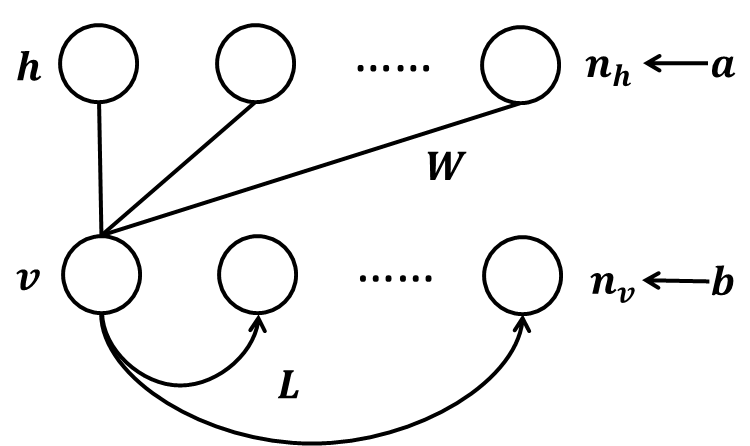
\includegraphics[width=\textwidth]{images/half_limit_and_limit_Boltzmann_machine_net_structure1.jpg}
        \caption{半限制}
        \label{fig:半限制}
    \end{subfigure}
    \quad
    \begin{subfigure}[b]{0.4\textwidth}
        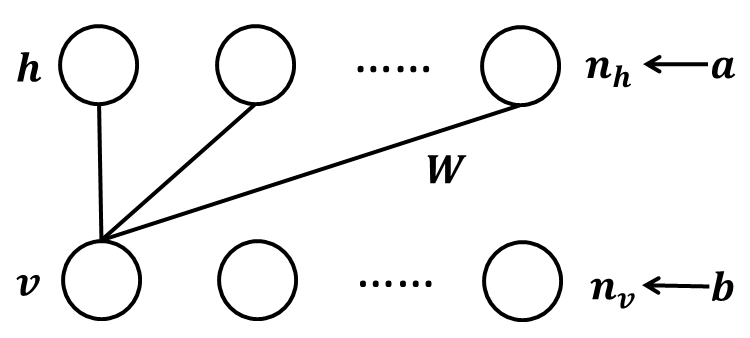
\includegraphics[width=\textwidth]{images/half_limit_and_limit_Boltzmann_machine_net_structure2.jpg}
        \caption{限制}
        \label{fig:限制}
    \end{subfigure}
    \caption{半限制和限制玻尔兹曼机网络结构图}
    \label{fig:半限制和限制玻尔兹曼机网络结构图}
\end{figure}
            关于$v,h,n_v,n_h,a,b,W,L$的符号说明如前所述,这里不再重述。对于(半)限制玻尔兹曼机,我们可以写出其能量函数$E(v,h)$
            \begin{align*}
            & E(v,h) = -v^\mathrm{T}Wh - \frac{1}{2} v^\mathrm{T}Lv - h^\mathrm{T}a - v^\mathrm{T}b\\
            & E(v,h) = -v^\mathrm{T}Wh - \frac{1}{2} v^\mathrm{T}Lv
            \end{align*}
            \par
            下面,我们仅讨论限制玻尔兹曼机RBM。RBM处于某一状态$(v,h)$的概率为
            \begin{align*}
            p(v,h) = \frac{1}{Z} e^{-E(v,h)}
            \end{align*}
            其中:$Z$为归一化因子,$Z = \sum_v\sum_he^{-E(v,h)}$包含$2^{n_v\times n_h}$项求和。RBM取值某一样本$v^k$的概率为
            \begin{align*}
            p(v^k) = \sum_h p(v^k,h) = \frac{1}{Z}\sum_he^{-E(v^k,h)}
            \end{align*}
            用极大似然估计法来估计参数$\theta$,求$\theta$使样本的联合概率密度(似然函数)最大,有
            \begin{align*}
            \max_{W,a,b} \ L(W,a,b) = P(v^1,v^2,\dots,v^m) = \prod_{k=1}^mp(v^k)
            \end{align*}
            取对数,有
            \begin{align*}
            \max_{W,a,b} \ \ln L(W,a,b) = \sum_{k=1}^m \log p(v^k)
            \end{align*}
            将$\ln L(W,a,b)$关于参数$\theta\triangleq (W,a,b)$求导,有
            \begin{align*}
            \frac{\partial \ln L}{\partial \theta} = \sum_{k=1}^m \frac{\partial \ln p(v^k)}{\partial \theta}
            \end{align*}
            而
            \begin{align}
            \label{RBM极大似然求导}
            \frac{\partial \ln p(v^k)}{\partial \theta} & = -\sum_h p(h|v^k )\frac{\partial E(v^k,h)}{\partial \theta} + \sum_{v,h}p(v,h)\frac{\partial E(v,h)}{\partial \theta} \\
             & = - \mathbb{E}_{p(h|v^k)} \left[ \frac{\partial E(v^k,h)}{\partial\theta}  \right] + \mathbb{ E}_{p(v,h)} \left[ \frac{\partial E(v,h)}{\partial \theta}  \right] \notag
            \end{align}
            \par
            下面,我们来分析(\ref{RBM极大似然求导})式右边第二项$\sum_{v,h}p(v,h)\frac{\partial E(v,h)}{\partial \theta}$
            \begin{align*}
            & \sum_{v,h}p(v,h)\frac{\partial E(v,h)}{\partial \theta} \\
            ={}& \sum_v\sum_hp(v)p(h|v)\frac{\partial E}{\partial \theta}\\
            ={}& \sum_vp(v)\sum_hp(h|v)\frac{\partial E}{\partial \theta}
            \end{align*}
            因此,只要求出$\sum_hp(h|v)$即可,即$p(h|v)$。前面我们提到过,只要隐含层层内各神经元之间不连接(即相互独立),则有
            \begin{align*}
            p(h|v) = \prod_{j=1}^{n_h}p(h_j|v)
            \end{align*}
            并且,对RBM有(在半限制玻尔兹曼机则不成立)
            \begin{align*}
            p(h_j|v ,h_{-j}) = p(h_j|v)
            \end{align*}
            同理,在RBM中
            \begin{align*}
            p(v|h) = \prod_{i=1}^{n_v}p(v_i|h)
            \end{align*}
            并且如果设置激励函数/传递函数为sigmoid:$p(v_i=1|h) = \sigma(b_i +W_{i:}h)$,则有
            \begin{align*}
            p(v|h) = \prod_{i=1}^{n_v}p(v_i|h)=  \prod_{i=1}^{n_v}\sigma(b_i +W_{i:}h)
            \end{align*}
            我们将$\theta$还原为$(W,a,b)$,于是有下面的关于$W_{ij},a_i,b_i$的导数情况\\
            (1)关于$W_{ij}$的导数
            \begin{align*}
            &\sum_hp(h|v) \frac{\partial E}{\partial W_{ij}}\\
            ={}& \sum_h\prod_{i=1}^{n_h}p(h_i|v)\frac{\partial E}{\partial W_{ij}}\\
            ={}& \sum_h p(h_i|v)p(h_{-i}|v)\frac{\partial E}{\partial W_{ij}}\\
            \xlongequal{\frac{\partial E}{\partial W_{ij}} = -h_iv_j} {}&-\sum_hp(h_i|v)p(h_{-i}|v)h_iv_j\\
            ={}&-\sum_{h_i}\sum_{h_{-i}}p(h_i|v)p(h_{-i}|v)h_iv_j\\
            ={}&-\sum_{h_i}p(h_i|v)h_iv_j\sum_{h_{-i}} p(h_{-i}|v)\\
            \xlongequal{\sum_{h_{-i}}p(h_{-i}|v) = 1} {}& -\sum_{h_i}p(h_i|v)h_iv_j\\
            ={}&-\left[ p(h_i=0|v)\cdot 0\cdot v_j+p(h_i = 1|v) \cdot 1\cdot v_j \right]\\
            ={}& -p(h_i=1|v)v_j
            \end{align*}
            (2)关于$b_i$的导数
            \begin{align*}
            & \sum_hp(h|v)\frac{\partial E}{\partial b_i}\\
            ={}& -\sum_hp(h|v)v_i\\
            ={}& v_i
            \end{align*}
            其中:$\frac{\partial E}{\partial b_i} = -v_i$,$\sum_h p (h|v)=1$。\\
            (3)关于$a_i$的导数(类似于$W_{ij}$的情况)
            \begin{align*}
            &\sum_hp(h|v) \frac{\partial E}{\partial a_i}\\
            ={}&-p(h_i=1|v)
            \end{align*}
            \par
            对于(\ref{RBM极大似然求导})式,我们已经求出等号右边第二项,于是有
            \begin{align*}
            & \begin{aligned}
            \frac{\partial \ln p(v^k)}{\partial W_{ij}}
            & = -\sum_hp(h|v^k)\frac{\partial E(v^k,h)}{\partial W_{ij}}+ \sum_{v,h} p(v,h)\frac{\partial E(v,h)}{\partial W_{ij}}\\
            & =p(h_i=1|v^k)v_j^k - \sum_vp(v)p(h_i = 1|v)v_j
            \end{aligned}\\
            & \frac{\partial \ln p(v^k)}{\partial b_i} = v_i^k- \sum_vp(v)v_i\\
            & \frac{\partial \ln p(v^k)}{\partial a_i} = p(h_i=1|v) - \sum_vp(v)p(h_i=1|v)
            \end{align*}
            其中:
            \begin{align*}
            p(h_j = 1|v,h_{-j}) = p(h_j=1|v) = \sigma(a_j+v^\mathrm{T}W_{:j})
            \end{align*}
            $W_{:j}$表示权重矩阵$W$的第$j$列,可写为$W_j,W_{\cdot j}$或者$W_{:,j}$。
            \begin{remark}
            在BM中,已经说明了$p(x_i=1) = \sigma(\sum_jW_{ij}x_j + \theta_i)$。
            这里,我们再用另一种方法推导。要求$p(h_j=1|v)$,令$h_{-j} = (h_1,h_2,\dots,h_{k-1},h_{k+1},\dots,h_{n_h})^\mathrm{T}$,并令
            \begin{align*}
            & \alpha_j(v) = b_j + \sum_{i = 1}^{n_v}v_i W_{ij}\\
            & \beta(v,h_{-j}) = \sum_{i=1}^{n_v}a_iv_i + \sum_{k\neq j}^{n_h}b_kh_k+\sum_{i=1}^{n_v}\sum_{k\neq j}^{n_h}v_i W_{ik}h_k\\
            & E(v,h) = -\beta(v,h_{-j}) - h_{-j}\alpha_j(v)
            \end{align*}
            于是有
            \begin{align*}
            p(h_j = 1|v)={}& p(h_j=1|h_{-j},v)\\
            ={}& \frac{p(h_j = 1|h_{-j},v)}{p(h_{-j},v)}\\
            ={}& \frac{p(h_j=1,h_{-j},v)}{p(h_j  =1,h_{-j},v)+ p(h_j  =0,h_{-j},v)}\\
            ={}& \frac{\frac{1}{2}e^{-E(h_j=1,h_{-j},v)}}{\frac{1}{2}e^{-E(h_j=1,h_{-j},v)} + \frac{1}{2}e^{-E(h_j=0,h_{-j},v)}}\\
            ={}& \frac{1}{1+ e^{- E(h_j=0,h_{-j},v)+ E(h_j=1,h_{-j},v)}}\\
            ={}& \frac{1}{e^{[\beta(v,h_{-j},v)+ 0\cdot \alpha _j(v)] + [-\beta(v,h_{-j}) - 1\cdot \alpha_j(v)]}}\\
            ={}& \frac{1}{-\alpha_j(v)}\\
            ={}& sigmoid(\alpha_j(v))\\
            ={}& sigmoid \left( b_j + \sum_{i=1}^{n_v}v_iW_{ij} \right) \\
            ={}& \sigma \left( b_j + \sum_{i=1}^{n_v}v_iW_{ij} \right)
            \end{align*}
            $\square$
            \end{remark}
            \par
            由
            \begin{align*}
            \frac{\partial \ln L}{\partial \theta} = \sum_{k=1}^m\frac{\ln p(v^k)}{\partial \theta}
            \end{align*}
            得到$m$个样本的导数(不仅可以使用一个样本、$m$个样本,还可以使用批量样本mini batch),为
            \begin{align*}
            &\frac{\partial \ln L}{\partial W_{ij}} = \sum_{k=1}^m \left[ p(h_i=1|v^k)v_j^k - \sum_vp(v)p(h_i = 1|v)v_j \right]\\
            &\frac{\partial \ln L}{\partial b_i} = \sum_{k=1}^m \left[ v_i^k- \sum_vp(v)v_i \right]\\
            &\frac{\partial \ln L}{\partial a_i} = \sum_{k=1}^m \left[  p(h_i=1|v) - \sum_vp(v)p(h_i=1|v) \right]
            \end{align*}
            最终,有参数的更新公式
            \begin{align*}
            \theta :=\theta + \eta\Delta\theta
            \end{align*}

        \subsubsection{RBM学习算法}
            \par
            RBM模型可以使用前面BM的Gibbs simple、变分近似法以及随机逼近SAP等方法进行求解。G.E.Hinton于2002年提出一种更离散的算法:k-CD(Contrastive Divergence),在Hinton的个人主页上可以找到相应的M文件。在k-CD之后,又相继出现了持续对比散度PCD以及快速持续对比散度FPCD等改进算法。下面,我们主要介绍CD算法和PCD算法。
            \paragraph{k-CD算法}通过上面的分析我们知道,权重$W_{ij}$的更新公式为
            \begin{align*}
            \frac{\partial \ln L}{\partial W_{ij}} = - \left[ \big< v_ih_j \big>_{data} -\big< v_ih_j \big>_{model}\right]
            \end{align*}
            其中:$\langle \cdot \rangle_{data}$和$\langle \cdot \rangle_{model}$分别是从数据和最终模型中估计$\cdot$的期望值。第一个期望$\big< v_ih_j \big>_{data}$是样本数据中可视层$v_i$和隐含层$h_j$同时为1的频率,而$\big< v_ih_j \big>_{model}$是以最终模型定义的分布来求得的频率。在吉布斯采用中,用$\big< v_ih_j \big>_{\infty}$来近似$\big< v_ih_j \big>_{model}$,然而,运行很多步($d$次)吉布斯采样器是低效的,为此,我们只运行1步($k$步)吉布斯采样,用一个非常粗略的$\big< v_ih_j \big>_{1}$来估计$\big< v_ih_j \big>_{modal}$
            \begin{align*}
            \big< v_ih_j \big>_{model} \approx \big< v_ih_j \big>_{1} = v_i^1h_j^1
            \end{align*}
            然而,$\big< v_ih_j \big>_{1}$具有很大的方差,为了减小方差,可以用下面的方法来估计$\big< v_ih_j \big>_{model}$
            \begin{align*}
            & h^0 \sim p(h,v^0)\\
            & v^1 = \mathbb{E}(v|h^0) = p(v|h^0)\\
            & h^1 = \mathbb{E}(h|v^1) = p(h|v^1)
            \end{align*}
            其中:$\sim$表示采样,$v^0$为一个样本。如果使用$N$步对比散度($N$通常较小),生成可视层向量的时候,都可以使用期望值,需要隐含层向量时,除了最后一次使用期望向量外,都可以使用采样技术。N-CD算法的伪代码如下(\ref{code:CD})
            \begin{algorithm}[htbp]
                \caption{N - CD for RBM}\label{code:CD}
                \begin{algorithmic}[1]
                    \State 初始化:样本集$D_m = \{v^k\}_{k=1}^m$,$N$,初始权重$W_0,a_0,b_0$,容许误差$\varepsilon$,学习率$\eta$。
                    \While {未达到停止准则}
                        \State $//$停止准则可以是最大迭代次数或者梯度$\Delta W < \varepsilon$。
                        \State 随机挑选$M_b$个样本的小批量$O = \left\{v^{(1)},v^{(2)},\dots,v^{(M_b)}\right\}$,进行如下计算
                        \begin{align*}
                        & \Delta W \leftarrow \frac{1}{M_b}\sum_{t=1}^{M_b}v^{(t)}\hat{h}^{(t)}{}^\mathrm{T}\\
                        & \Delta b \leftarrow \frac{1}{M_b}\sum_{t=1}^{M_b}v^{(t)}\\
                        & \Delta a \leftarrow \frac{1}{M_b}\sum_{t=1}^{M_b}\hat{h}^{(t)}
                        \end{align*}
                        \For {$t=1$ to $M_b$}
                            \State $\tilde{v}^{(t)} \leftarrow v^{(t)}$
                        \EndFor
                        \For {$n \gets 0;n<N;n \gets n+1$ }
                            \For {$t = 1$ to $M_b$}
                                \State $\tilde{h}^{(t)}$ sampled from
                                $\prod_{j=1}^{n_h}\sigma \left( a_j+\tilde{v}^{(t)}{}^\mathrm{T} W_{:j} \right) $
                                \State $\tilde{v}^{(t)}$ sampled from
                                $\prod_{j=1}^{n_v}\sigma \left( b_i+W_{i:}\tilde{h}^{(t)} \right)$
                            \EndFor
                        \EndFor
                        \State 计算
                        \begin{align*}
                        & \bar{h}^{(t)} \leftarrow \sigma \left( a+ \tilde{v}^{(t)}{}^\mathrm{T}W \right) \\
                        & \Delta W \leftarrow \Delta W - \frac{1}{M_b}\sum_{t=1}^{M_b} \tilde{v}^{(t)}\bar{h}^{(t)}{}^\mathrm{T}\\
                        & \Delta b \leftarrow \Delta b - \frac{1}{M_b}\sum_{t=1}^{M_b} \tilde{v}^{(t)}\\
                        & \Delta a \leftarrow \Delta a - \frac{1}{M_b}\sum_{t=1}^{M_b} \bar{h}^{(t)}
                        \end{align*}
                        \State 更新权重
                        \begin{align*}
                        & W \leftarrow W + \eta \Delta W\\
                        & b \leftarrow b+ \eta \Delta b\\
                        & a \leftarrow a+ \eta \Delta a
                        \end{align*}
                    \EndWhile
                    \State 输出:$W,a,b$.
                \end{algorithmic}
            \end{algorithm}

            \paragraph{PCD算法} Tideman提出PCD算法,弥补了CD算法无法极大化似然函数的缺陷。大量实验表明,PCD算法训练的RBM具有更好的学习能力。PCD算法从持续马尔科夫链得到负阶段样本来近似梯度。令$t$步的持续马尔科夫链为$v_t$,梯度的更新规则为
            \begin{align*}
            \Delta \theta = \eta \left( \mathbb{E}(vh_0^\mathrm{T}) - \mathbb{E}(\tilde{v}_{t+k} \tilde{ h}_{t+k}^\mathrm{T}) \right)
            \end{align*}
            其中:$\tilde{v}_{t+k},\tilde{h}_{t+k}$是从状态$\tilde{v}$开始进行$k$个持续马尔科夫链步骤得到的样本。PCD伪代码如下(\ref{code:PCD})
            \begin{algorithm}[htbp]
                \caption{PCD for RBM}\label{code:PCD}
                \begin{algorithmic}[1]
                    \State 初始化:样本集$D_m = \{v^k\}_{k=1}^m$,$N$,初始权重$W_0,a_0,b_0$,容许误差$\varepsilon$,学习率$\eta$,Gibbs steps $N$,初始虚拟样本$\{\tilde{v}^k\}_{k=1}^m$。
                    \While {未达到停止准则}
                        \State $//$停止准则可以是最大迭代次数或者梯度$\Delta W < \varepsilon$。
                        \State 从样本集$D_m$中随机挑选$M_b$个样本的小批量$O = \left\{v^{(1)},v^{(2)},\dots,v^{(M_b)}\right\}$。进行如下计算
                        \begin{align*}
                        & \Delta W \leftarrow \frac{1}{M_b}\sum_{t=1}^{M_b}\hat{h}^{(t)}{v^{(t)}}^\mathrm{T}\\
                        & \Delta b \leftarrow \frac{1}{M_b}\sum_{t=1}^{M_b}v^{(t)}\\
                        & \Delta a \leftarrow \frac{1}{M_b}\sum_{t=1}^{M_b}\hat{h}^{(t)}
                        \end{align*}
                        \For {$n \gets 0;n<N;n \gets n+1$ }
                            \For {$t = 1$ to $M_b$}
                                \State $\tilde{h}^{(t)}$ sampled from
                                $\prod_{j=1}^{n_h}\sigma \left( a_j+\tilde{v}^{(t)}{}^\mathrm{T} W_{:j} \right) $
                                \State $\tilde{v}^{(t)}$ sampled from
                                $\prod_{j=1}^{n_v}\sigma \left( b_i+W_{i:}\tilde{h}^{(t)} \right) $
                            \EndFor
                        \EndFor
                        \State 计算
                        \begin{align*}
                        & \Delta W \leftarrow \Delta W - \frac{1}{M_b}\sum_{t=1}^{M_b} \tilde{v}^{(t)}\tilde{h}^{(t)}{}^\mathrm{T}\\
                        & \Delta b \leftarrow \Delta b - \frac{1}{M_b}\sum_{t=1}^{M_b} \tilde{v}^{(t)}\\
                        & \Delta a \leftarrow \Delta a - \frac{1}{M_b}\sum_{t=1}^{M_b} \tilde{h}^{(t)}
                        \end{align*}
                        \State 更新权重
                        \begin{align*}
                        & W \leftarrow W + \eta \Delta W\\
                        & b \leftarrow b+ \eta \Delta b\\
                        & a \leftarrow a+ \eta \Delta a
                        \end{align*}
                    \EndWhile
                    \State 输出:$W,a,b$.
                \end{algorithmic}
            \end{algorithm}

% \bibliography{part-MLDL-chap-ANN}%bib文件名称
% \end{document}
